\documentclass[a4paper,10pt,german]{scrbook}

\usepackage{latexki}
\lecturer{Prof. Dr. F. Herrlich}
\semester{Wintersemester 07/08}
\scriptstate{partial}

\usepackage[OT1,T1]{fontenc}
\usepackage{babel}
\usepackage{cmbright}
\usepackage{url}
\usepackage{makeidx}
\usepackage{framed}
\usepackage[pdftex]{xcolor}

\usepackage[utf8]{inputenc}

\usepackage{stmaryrd}
%\usepackage{ulsy}
%blitztest
\newcommand{\blitza}[0]{\lightning}
\newcommand{\blitzb}[0]{\lightning}
\newcommand{\blitzc}[0]{\lightning}
\newcommand{\blitzd}[0]{\lightning}

%erstmal auskommentiert, leider kann das amscd-Paket nicht so viel :/
%\usepackage{pictexwd,dcpic}

\usepackage{colortbl}

\usepackage{hyperref}

% Mathe-Pakete
\usepackage{amssymb}
\usepackage{amsmath}
\usepackage{amsfonts}
\usepackage{amsthm}
\usepackage{amscd}
\usepackage{mathtools}
\usepackage{faktor}

\usepackage{graphicx}

%\usepackage{algebra}
\newcommand{\da}{\coloneqq}
\newcommand{\ad}{\eqqcolon}


\newtheoremstyle{saetze}% Name des Stils
{3pt}% vertikaler Abstand zum vorangehenden Text
{3pt}% vertikaler Abstand zum folgenden Text
{}% Schriftart des Textkörpers
{}% Abstand des Erstzeileneinzugs der Kopfzeile
{\Large \bfseries}% Schriftart des Kopfes
{}% Punktierung nach dem Kopf
{\newline}% Abstand nach dem Kopf (z.B. \newline)
{}% Kopfspezifikation (leer bedeutet 'normal')

\newtheoremstyle{definitionen}% Name des Stils
{3pt}% vertikaler Abstand zum vorangehenden Text
{3pt}% vertikaler Abstand zum folgenden Text
{}% Schriftart des Textkörpers
{}% Abstand des Erstzeileneinzugs der Kopfzeile
{\large \bfseries}% Schriftart des Kopfes
{}% Punktierung nach dem Kopf
{\newline}% Abstand nach dem Kopf (z.B. \newline)
{}% Kopfspezifikation (leer bedeutet 'normal')

\theoremstyle{saetze}
    \newtheorem{Satz}{Satz}
    
\theoremstyle{definitionen}
    \newtheorem{Def}{Definition}[section]
    \newtheorem{DefBem}[Def]{Definition + Bemerkung}
    \newtheorem{Bem}[Def]{Bemerkung}
    \newtheorem{BemDef}[Def]{Bemerkung + Definition}
    \newtheorem{Prop}[Def]{Proposition}
    \newtheorem{PropDef}[Def]{Proposition + Definition}
    \newtheorem{Folg}[Def]{Folgerung}
    \newtheorem{Bsp}[Def]{Beispiel}
    \newtheorem{Bspe}[Def]{Beispiele}
    \newtheorem{DefProp}[Def]{Definition + Proposition}

\title{Algebra I}
\author{Prof. Dr. F. Herrlich}
\publishers{Die Mitarbeiter von \url{http://mitschriebwiki.nomeata.de/}}
\makeindex

\begin{document}


\setkomafont{sectioning}{\normalfont\normalcolor\bfseries}
\setkomafont{descriptionlabel}{\normalfont\normalcolor\bfseries}

%\renewcommand*{\othersectionlevelsformat}[1]{\llap{\csname the#1 \endcsname\autodot\enskip}}

%\newcommand{\ssubsection}[1]{\subsection{#1 \thesubsection} \label{\thesubsection}}

\newcommand{\emp}[1]{\textbf{\emph{#1\index{#1}}}}
\newcommand{\empind}[2]{\textbf{\emph{#1\index{#2}}}}

\newenvironment{define}
    { \begin{flushleft} \begin{description} }
    { \end{description} \end{flushleft} }

\newenvironment{enum} {
      \begin{enumerate}
      \renewcommand{\labelenumi}{(\alph{enumi})}

      }
      { \end{enumerate} }

\newcommand{\bla}[0]
{\begin{tiny} $\left\{
\begin{array}{l}
             . \\
             . \\
             . \end{array}
        \right\}$
\end{tiny}}

\newcommand{\blab}[0]
{\begin{tiny} $\left\{
\begin{array}{l}
             Halbgruppen \\
             Monoiden \\
             Gruppen \end{array}
        \right\}$
\end{tiny}}


\newenvironment{ourshaded}{%
  \def\FrameCommand{\colorbox{shadecolor}}%
  \edef\frmlw{\linewidth}%
  \MakeFramed{\setlength\hsize{\linewidth}\FrameRestore}%
  \setlength{\parskip}{1em}\setlength{\parindent}{0pt}}{\endMakeFramed}

\newcommand{\bew}[2]
{\definecolor{shadecolor}{rgb}{0.85,0.85,1}
 \begin{shaded}
 \textit{\textbf{Beweis: }}
 #1
 \begin{enum} #2
 \hfill \rule{2,1mm}{2,1mm} \end{enum}
 \end{shaded}
}

\newcommand{\sbew}[1]
{\definecolor{shadecolor}{rgb}{0.85,0.85,1}%
 \begin{ourshaded}%
 \textit{\textbf{Beweis:}} #1%
 \hfill \rule{2,1mm}{2,1mm}%
 \end{ourshaded}
}

\newcommand{\bsp}[1]
{\definecolor{shadecolor}{rgb}{0.85,1,0.85}%
 \begin{ourshaded}%
 \textit{\textbf{Beispiel:}} #1%
 \end{ourshaded} 
}

\newcommand{\ra}[0]{\rightarrow}
\newcommand{\ds}[0]{\displaystyle}
\newcommand{\cd}[0]{\cdot}
\newcommand{\lra}[0]{\Leftrightarrow}
\newcommand{\Ra}[0]{\Rightarrow}

\newcommand{\para}[1]{\noindent \Large\textbf{#1} \normalsize}

\newcommand{\defeqr}[0]{\mathrel{\mathop:}=}
\newcommand{\defeql}[0]{=\mathrel{\mathop:}}

\newcommand{\chk}[0]{\checkmark}
\newcommand{\wt}[0]{\widetilde}

\newcommand{\Kern}{\mathop{\rm Kern}\nolimits}
\newcommand{\Bild}{\mathop{\rm Bild}\nolimits}
\newcommand{\ord}{\mathop{\rm ord}\nolimits}

\maketitle

\addcontentsline{toc}{chapter}{Inhaltsverzeichnis}
\tableofcontents


\chapter{Gruppen}

\section{Grundlegende Definitionen}

\begin{Def} 
    Sei $M$ eine Menge.

    \begin{enum}
        \item Eine \emp{Verknüpfung} auf $M$ ist eine Abbildung $\cd: M
              \times M \ra M $

        \item Eine Menge $M$ zusammen mit einer Verknüpfung $\cd$ heißt
              \emp{Magma}.

        \item Eine Verknüpfung $\cd : M \times M \ra M$ heißt \emp{assoziativ},
        wenn \[\forall x,y,z \in M: (x\cd y)\cd z=x\cd(y\cd z)\]

        \item Eine \emp{Halbgruppe} ist ein assoziatives Magma.
    
        \item $e \in M$ heißt \emp{neutrales Element} für die Verknüpfung $\cd$,
        wenn \[\forall x \in M: x \cd e = e \cd x = x\]
          
        \item Eine Halbgruppe mit neutralem Element heißt \emp{Monoid}.

        \item Eine \emp{Gruppe} ist ein Monoid $(G,\cd)$, in dem es zu jedem $x
        \in G$ ein $x' \in G$ gibt mit \[ x \cd x' = x' \cd x = e \] $x'$ heißt
        dann \emp{zu $x$ inverses Element.}
    \end{enum}
\end{Def}

\begin{Bem}
    Sei $(M,\cd)$ ein Magma.
    
    \begin{enum}
        \item In $M$ gibt es höchstens ein neutrales Element.
        \sbew{Sind $e, e'$ neutrale Elemente, so ist $e=e\cd e' = e'$}

        \item Ist $M$ Monoid, so gibt es zu $x \in M$ höchstens ein inverses 
        Element.
        \sbew{Seien $x',x''$ zu $x$ invers, so ist $x'=(x'' \cd x)\cd x' =
        x'' \cd (x \cd x')=x''$}
    \end{enum}
\end{Bem}

\begin{DefBem} 
    Sei $(M,\cd)$ ein(e)
    \begin{small} $\left\{ \begin{array}{l}
            Magma \\
            Halbgruppe \\
            Monoid \\
            Gruppe \end{array}
    \right\}$
    \end{small}

    \begin{enum}
        \item $U \subseteq M$ heißt Unter-\bla, wenn $U \cd U \subseteq U$ und
        $(U,\cd)$ selbst ein(e) \bla ist.
        
        \item $U \subseteq M$ Unterhalbgruppe $\Leftrightarrow U \cd U \subseteq
        U$
        
        \item $U \subseteq M$ Untermonoid $\lra U \cd U \subseteq U$ und $e \in
        U$
        
        \item $U \subseteq M$ Untergruppe $\lra U \neq \emptyset$ und $\forall
        x,y \in U: x \cd y^{-1} \in U$
	\sbew{''$\Leftarrow$'': \newline Sei $x \in U \> \Rightarrow e=x \cd x^{-1}
        \in U \Rightarrow $ mit $x$ ist auch $x^{-1}$ in $U \Rightarrow$ mit
        $x,y$ ist auch $xy = x(y^{-1})^{-1} \in U$}
    \end{enum}
\end{DefBem}

\begin{Bem} 
    Sei $ (M,\cd)$ Monoid. Dann ist $M^x \defeqr \{x \in M:$ es gibt inverses
    $x^{-1}$ zu $x \in M\}$ eine Gruppe.
    \sbew{ $\\e \in M^x$, da $e\cd e = e$, also $M^x \neq \emptyset$.
    Sind $x,y \in M^x$, so ist $x \cd y \in M^x$, da $xy \cd
    (y^{-1}x^{-1})=e \Rightarrow \cd$ ist Verknüpfung auf $M^x \Rightarrow
    (M^x, \cd)$ ist Gruppe.}
\end{Bem}

\begin{DefBem}
    Seien $(M, \cd), (M',*)$ \bla
    \begin{enum}
        \item Eine Abbildung $f:M\ra M'$ heißt \emp{Homomorphismus}, wenn
        $\forall \; x,y \in M:\\\\$ \bigskip $ f(x\cd y) = f(x)*f(y)$ \hfill
        \textmd{(i)} \newline Hat M ein neutrales Element, so muß außerdem
        gelten: $\\\\f(e) = e'$ \hfill \textmd{(ii)}
        
        \item Ist $f:G \ra G'$ Abbildung von Gruppen, die \textmd{(i)} erfüllt,
        so ist $f$ Homomorphismus.
	\sbew{ $f(e) = f(e \cd e) =
        f(e) * f(e) \overset{\cd f(e)^{-1}}{\Rightarrow} e' = f(e)$} 
        
        \item Ein Homomorphismus $f:M \ra M'$ heißt \emp{Isomorphismus}, wenn es
        einen Homomorphismus $g:M'\ra M$ gibt, mit $f \circ g = id_{M'}$ und $g
        \circ f = id_M$

        \item Jeder bijektive Homomorphismus ist Isomorphismus. \newline
        \sbew{Sei $f:M\ra M'$ bijektiver Homomorphismus und $g:M' \ra M$
        die Umkehrabbildung. z.z.: $g$ ist Homomorphismus. \newline Seien $x,y
        \in M'$. Schreibe $x=f(\hat{x}), y=f(\hat{y})$ für passende $\hat{x},\hat{y} \in M 
        \Rightarrow g(x\cd y) = g(f(\hat{x}) \cd f(\hat{y})) = g(f(\hat{x} \cd \hat{y})) = 
        \hat{x} \cd \hat{y} = g(f(\hat{x})) \cd g(f(\hat{y})) = g(x) \cd g(y) $}

        \item Die Komposition von Homomorphismen ist wieder ein Homomorphismus.
    \end{enum}
\end{DefBem}

\begin{Def} 
    Sei $f:M \ra M'$ Hom von \bla.
    
    \begin{enum}
        \item $\Bild(f) \defeqr \{f(x):x \in M\} \subseteq M'$ ist ein
        Unter-\bla. 
        \sbew{Sind $x,x' \in M$, so ist $f(x)*f(x')=f(x \cd x') \in 
        \Bild(f)$. Sind $M,M'$ Monoide, so gilt: $f(e) = e' \in$ $\Bild(f)$.
        Sind $M, M'$ Gruppen, so gilt: $f(x)^{-1} = f(x^{-1}) \in$ $\Bild(f)$, da
        $f(x\cd x^{-1}) = f(e) = e' = f(x) * f(x^{-1})$}
        
        \item Sind $M, M'$ Monoide/Gruppen, so ist $\Kern(f) \defeqr \{x \in M :
        f(x) = e'\}$ Untermonoid/-gruppe von $M$. 
        \sbew{$x,y \in$ $\Kern(f) \Rightarrow f(xy) = f(x) * f(y) = e'*e' =
        e' \Rightarrow xy \in$ $\Kern(f), e \in$ $\Kern(f) \;\chk$ \\
        $x\in$ $\Kern(f) \Rightarrow f(x^{-1}) = f(x)^{-1} = (e')^{-1} = e'
        \Rightarrow x^{-1} \in$ $\Kern(f)$}

        \item Sind $G,G'$ Gruppen, so ist $f$ genau dann injektiv, wenn $\Kern(f)
        = \{e\}$
    \end{enum}
\end{Def}

\section{Beispiele und Konstruktionen}

\begin{enum}
    \item[(1)] Sei $M$ eine Menge. $\\M^M \defeqr \{ f:M \ra M$ Abbildung $\}$
    ist mit der Verknüpfung $\cd$ ein Monoid. $(M^M)^X = \{f: M \ra M$ bijektiv
    $\} \defeql$ Perm$(M) = S_M$. \newline
    insbesondere: $M=\{1,\dots ,n\}: S_{ \{1, \dots, n\} } = S_n$ Ist $(M,\cd)$
    ein \bla, so ist $End(M) \defeqr \{f \in M^M :f\;$ Hom.$\}$ ein Untermonoid
    von $M^M$ und \newline
    $Aut(M) \defeqr$ Perm$(M) \cap$ End$(M)$ Untergruppe von Perm$(M)$

    \item[(2a)] Sei $X$ Menge, $M$ ein(e) \bla. Dann ist $M^X = \{f:X \ra M$
    Abbildung $\}$ mit der Verknüpfung $(f\cd g)(x) = f(x)\cd g(x)$ ein(e) \bla
    
    \item[(2b)] Ist $(M,\cd)$ Halbgruppe, $(H,+)$ kommutative Halbgruppe, so
    ist Hom$(M,H) \defeqr \{f \in H^M: f\;$ Homomorphismus$\}$ eine kommutative
    Unterhalbgruppe von $H^M$. \newline\textbf{denn}: Sind $f,g: M \ra H$
    Homomorphismen, so ist $\forall x,y \in M$: \newline
    $(f+g)(x\cd y) = f(x \cd y) + g(x \cd y) = f(x) + f(y) + g(x) + g(y) = f(x)
    + g(x) + f(y) + g(y) = (f + g)(x) + (f + g)(y)$

    \item[(3)] Sei $I$ eine Indexmenge. Für jedes $i \in I$ sei $(M_i, \cd)$
    ein(e) \bla.
    \begin{enum}
        \item $\displaystyle \prod_{i \in I} M_i$ ist mit komponentenweiser
        Verknüpfung ein(e) \bla.
        
        \item Sind $M_i$ Monoide, so ist \[ \bigoplus_{i \in I} M_i \defeqr \{ 
        (x_i)_{i \in I} \in \prod_{i \in I} M_i, x_i = e_i \mbox{ ffa.} i\}\]
        ein Monoid.
    \end{enum}
\end{enum}

\begin{DefBem}
\mbox{}
\begin{enum}
\item $\prod$ heißt \emp{direktes Produkt} \newline
$\bigoplus$ heißt \emp{direkte Summe}
\item Ist $I$ endlich, so ist $\prod M_i \cong \bigoplus M_i$
\item Sei $M$ ein(e) \bla und für jedes $i \in I: g_i:M \ra
M_i$ ein Homomorphismus. Dann gibt es genau einen Homomorphismus
$\displaystyle G:M \ra \prod_{i \in I} M_i$, so dass $g_i = pr_i
\circ G$, wobei $\displaystyle pr_i: \prod_{j \in I} M_j \ra M_i$
Projektion.

%\[\begindc{\commdiag} \obj(1,1){$M$}
%                      \obj(5,1){$M_i$}
%                      \obj(3,3){$\pi M_j$}
%                      \mor{$M$}{$M_i$}{$g_i$}
%                      \mor{$M$}{$\pi M_j$}{$\exists!\;G$}[1,1]
%                      \mor{$\pi M_j$}{$M_i$}{pr$_i$}
%\enddc\]

\sbew{Setze $G(m) \defeqr (m_j)_{j \in I}$ mit $m_j =
g_j(m)$ für $m \in M$. $G$ ist Homomorphismus. $\chk\;\\$ $G$ ist
eindeutig, da $pr_i(G(m)) = g_i(m)$ sein muss.}
\item Ist $(M,+)$ ein kommutatives Monoid, und für jedes $i \in I\; f_i:M_i
\ra M$ ein Homomorphismus, so gibt es genau einen Homomorphismus \[
F: \bigoplus_{j\in I} M_j \ra M \mbox{, so dass für jedes } i \in I: f_i = F
\circ \nu_i \mbox{, wobei } \nu_i:M_i \ra \bigoplus_{j\in I} M_j\] \[m \mapsto
(m_j)_{j \in I}\mbox{, wobei } m_j = \left\{
\begin{array}{rl}
            m & i=j \\
            e_j & \mbox{sonst}
          \end{array}\right.\]

%\[\begindc{\commdiag} \obj(1,3){$M_i$}
%                      \obj(3,3){$M$}
%                      \obj(2,1){$\oplus_{j\in I} M_j$}
%                      \mor{$M_i$}{$M$}{$f_i$}
%                      \mor{$M_i$}{$\oplus_{j\in I} M_j$}{$\nu_i$}
%                      \mor{$M$}{$\oplus_{j\in I} M_j$}{$\exists!\;F$}[1,1]
%\enddc\]

\sbew{Setze $F((m_j)_{j \in I}) = \displaystyle \sum_{j \in I} f_j(m_j)$
\newline Brauche: $F((e,\dots, e,m_i,e,\dots,e)) = F(\nu_i(m_i)) \overset{!}{=}
f_i(m_i)$
\newline $\Rightarrow F((e,\dots,e,m_i,e,\dots,e,m_j,e,\dots,e)) = f_i(m_i) +
f_j(m_j) = F((e,\dots,e,m_i,e,\dots,e)) + F((e,\dots,e,m_j,e,\dots,e))$}

\end{enum}
\begin{enum}
\item[(4)] Sei $S$ eine Menge (''Alphabet'') $F^a(S) \defeqr
\displaystyle \bigcup^{\infty}_{n=1} S^n$ ist Halbgruppe mit Verknüpfung
''Nebeneinanderschreiben'' $\underset{\in S^n}{(x_1,\dots,x_n)}\cd
\underset{\in S^m}{(y_1,\dots,y_m)} \defeqr \underset{\in
S^{n+m}}{(x_1, \dots, x_n, y_1, \dots, y_m)}$ $F^a(S)$ heißt freie Halbgruppe oder ''Worthalbgruppe'' über
$S$.

Definiert man $S^0 \defeqr \{\varepsilon\}$, dann ist $F_0^a(S) \defeqr \bigcup_{n=0}^\infty S^n$ ein Monoid mit neutralem Element $\varepsilon$, dem „leeren Wort“. Für $S=\{1\}$ ist $F_0^a(S) = (\mathbb N_0,+)$.
\end{enum}
\end{DefBem}

\begin{Bem} 
Ist $(H,\cd)$ Halbgruppe, $f:S\ra H$ eine
Abbildung, so gibt es genau einen Homomorphismus $\varphi:F^a(S) \ra H$
mit $\varphi(s) = f(s)$ für alle $s\in S$, wobei man $S$ als $S^1\subset F^a(S)$ auffasst.

\sbew{Für $(x_1,\ldots,x_n)\in S^n$ muss gelten: $\varphi(x_1,\ldots,x_n) = \varphi(x_1)\cdot\cdots\cdot\varphi(x_n) = f(x_1)\cdot\cdots\cdot f(x_n)$. Also ist $\varphi$ eindeutig und existiert, da es so definiert werden kann.
}
\end{Bem}

\begin{BemDef}
\label{1.9}
Sei $(M,\cd)$ ein Monoid und $(G,\cd)$ eine Gruppe
\begin{enum} 

\item Für $x \in M$ ist $\varphi_x: \mathbb{N}_0
\to M$, $n \mapsto x^n$ ein Homomorphismus.

\item Für $g \in G$, so ist $\varphi_g: \mathbb{Z} \to G$, $n \mapsto g^n$
ein Gruppenhomomorphismus.

\item $\langle g \rangle \defeqr \Bild(\varphi_g)$ heißt die von
$g$ erzeugte \emp{zyklische Untergruppe} von $G$.

\item $G$ heißt zyklisch, wenn es ein $g\in G$ gibt mit $\langle g\rangle =G$.

\item $| \langle g \rangle |\in \mathbb N\cup\{\infty\}$ heißt \emp{Ordnung} von $g$

\item Ist $G$ endlich, so heißt $| G |$ die \emp{Ordnung} von $G$.
\end{enum}


%\begin{enum}
%\item[(6)] Sei $G$ Gruppe, für $g \in G$ sei $\tau_g:G \ra G$, $x\mapsto g \cd 
%x$ (''Linksmultiplikation'')\newline
%$\tau_g(e)=g \Rightarrow$ kein Gruppenhomomorphismus, $\tau_e = id_G$
%\end{enum}
\end{BemDef}

\begin{DefBem}[Satz von Cayley]
\mbox{}
\begin{enum}
\item Für $g\in G$ heißt die Abbildung $\tau_g:G\to G$, $h \mapsto gh$ die \emph{Linksmultiplikation} mit $g$.

\item Für jedes $g\in G$ ist $\tau_g$ bijektiv, da $\tau_{g^{-1}}$ die Umkehrabbildung ist.

\item Die Abbildung:
\[ \begin{array}{lcc}
    \tau    &   :   &   G \ra \mbox{Perm}(G) \\
            &       &   g \mapsto \tau_g
    \end{array} \]
ist ein injektiver Gruppenhomomorphismus. 
\bew{}{ \item[(1)]
$\tau_g \in$ Perm$(G) : \tau_g$ ist bijektiv mit Umkehrabbildung
$\tau_{g^{-1}}$
\item[(2)] $\tau$ ist Homomorphismus: $\tau(g_1 g_2) = \tau(g_1)
\circ \tau(g_2)$, denn: $\forall x \in G: \tau(g_1 \circ g_2)(x) = (g_1 g_2)x =
g_1(g_2 x) = \tau_{g_1}(\tau_{g_2}(x)) = (\tau_{g_1}
\circ \tau_{g_2})(x)$ \item[(3)] $\Kern(\tau)$ = $\{e\}$, denn ist
$\tau(g) = id_g$, so ist $\forall x \in G: \tau_g(x) = gx = x$, also $g = e$}
\end{enum}
\end{DefBem}

\begin{DefBem}
\label{kernundnormalteiler}
Sei $G$ Gruppe, $g \in G$
\begin{enum}
\item Die Abbildung $c_g:G \ra G, x \mapsto gxg^{-1}$ ist ein
\emp{Automorphismus}, sie heißt \emp{Konjugation} mit $g$.

\sbew{$c_g$ ist Homomorphismus: $c_g(x_1 x_2) = g(x_1
x_2)g^{-1} \\ c_g(x_1) c_g(x_2) = (g x_1 g^{-1})(g x_2 g^{-1}) = c_g(x_1)\cdot c_g(x_2) \\
c_g$ ist bijektiv: Die Umkehrabbildung ist $c_{g^{-1}}$ }

\item Die Abbildung $c:G \ra$ Aut$(G), g \mapsto c_g$ ist ein
Gruppenhomomorphismus.
\sbew{$\forall x \in G: c(g_1 g_2)(x) = (g_1
g_2)x(g_1 g_2)^{-1} = g_1(g_2 x g_2^{-1})g_1^{-1} = (c(g_1) \circ
c(g_2))(x)$ }

\item Die Elemente von $\Bild(c) \defeql$ Aut$_i(G)$ heißen \emp{innere
Automorphismen} von $G$.

\item $Z(G)\defeqr$ $\Kern(c)$ heißt \emp{Zentrum} von $G$. Es ist $Z(G) =
\{ g \in G:\forall x \in G:gx=xg \}$

\item Eine Untergruppe $N \subseteq G$ heißt \emp{Normalteiler} in
$G$, wenn $\forall g \in G: c_g(N) \subseteq N$.
Äquivalent: $\forall g \in G, x \in N: g x g^{-1} \in N$

\item Ist $f:G \ra G'$ Gruppenhomomorphismus, so ist $\Kern(f)$
Normalteiler in G.

\sbew{Sei $x \in$
$\Kern(f), g \in G$. Dann ist $f(g x g^{-1}) = f(g)
\underset{e'}{\underbrace{f(x)}} f(g)^{-1} = e'$.}

\item Aut$_i(G)$ ist Normalteiler in Aut$(G)$

\sbew{Sei $\varphi \in \mbox{Aut}(G), g\in G :
\mbox{z.z.: } \varphi \cd c_g \cd \varphi^{-1} \in \mbox{Aut}_i(g).
\\ \mbox{Es ist } (\varphi \cd c_g \cd \varphi^{-1})(x) =
\varphi(c_g(\varphi^{-1}(x))) = \varphi(g \cd \varphi^{-1}(x)\cd
g^{-1}) = \varphi(g) \cd \varphi(\varphi^{-1}(x)) \cd
\varphi(g^{-1}) = \varphi(g) \cd x \cd \varphi(g)^{-1} =
c_{\varphi(g)}(x) \Rightarrow \varphi \circ c_g \circ \varphi^{-1} =
c_{\varphi(g)} \in \mbox{Aut}_i(G)$}
\end{enum}
\end{DefBem}

\begin{DefBem}
\label{1.12}
Sei $G$ Gruppe, $H \subseteq
G$ Untergruppe. \begin{enum}
\item Für $g \in G$ heißt $g \cd H = \{g\cd h : h \in H\} =
\tau_g(H)$ \emp{Linksnebenklasse} von $G$ bzgl. $H$ und $H \cd g=
\{h \cd g : h \in H \}$ \emp{Rechtsnebenklasse}


\item Für $g_1$, $g_2 \in G$ gilt: $g_1 H \cap g_2 H \neq
\emptyset \lra g_1 H = g_2 H$

\sbew{Sei $ y = g_1
h_1 = g_2 h_2 \in g_1 H \cap g_2 H$ und $h1, h2, h \in H \Rightarrow g_1 = g_2
h_2 h_1^{-1} \Rightarrow g_1 h = g_2h_2h_1^{-1} \in g_2 H \Rightarrow g_1 H \subseteq g_2 H$, die Umkehrung
folgt analog.}
\item $H$ ist genau dann Normalteiler, wenn $\forall g\in G: g\cd H = H \cd g
$ 
\sbew{$gH = Hg \lra H =
gHg^{-1}$}

\item Alle Nebenklassen von $G$ bzgl. $H$ sind gleichmächtig.

\sbew{$\tau_g: \underset{e\cd H}{\underbrace{H}} \ra g\cd H, h
\mapsto g\cd h$ ist bijektiv.}
\item Die Anzahl der Linksnebenklassen bzgl. $H$ ist gleich der
Anzahl der Rechtsnebenklassen. Sie heißt \emp{Index} $[G:H]$ von $H$
in $G$. 
\sbew{Die Zuordnung \[\begin{array}{lcl}
    \{\mbox{Linksnebenklasse}\} & \ra & \{\mbox{Rechtsnebenklasse}\} \\
    g\cd H                      & \mapsto & H \cd g^{-1}
    \end{array}\]
ist \emp{wohldefiniert} und bijektiv.

\textbf{Wohldefiniertheit:} ist $g_1 H = g_2 H$, also $g_2 = g_1 h$
für ein $h \in H \Rightarrow Hg_2^{-1} = H(g_1 h)^{-1} = H\cd
h^{-1}g_1^{-1} = Hg_1^{-1}$}


\item
\emp{Satz von Lagrange:} Ist $G$ endlich, so ist
\[[G:H] = \frac{|G|}{|H|}\] \sbew{$G$ ist disjunkte Vereinigung
der $[G:H]$ Linksnebenklassen bzgl. $H$. Diese haben alle $|H|$
Elemente.} \label{\thesubsection \theenumiii}
\end{enum}
\end{DefBem}

\section{Quotientenbildung}

\begin{DefBem}
    \label{restklassendefinition}
    Sei $f: M \ra M'$ eine Abbildung von Mengen.
    
    \begin{enum}
        \item Die Relation $\sim_f$ auf $M: x \sim_f y \lra f(x) = f(y)$ ist
        eine Äquivalenzrelation.

        \item Für $x \in M$ sei $\bar x \defeqr [x]_f \defeqr \{ y \in M : y\sim_f x\} = \{ y\in M: f(y)= f(x)\}$.
	Es ist $\bar x = f^{-1}(f(x))$
	
	Weiter sei $\bar M \defeqr M/\sim_f \defeqr \{ \bar x : x \in M\}$

	\item $\bar f : \bar M\to \Bild(f)$, $\bar x\mapsto f(x)$ ist eine bijektive Abbildung.

    \end{enum}
\end{DefBem}

\begin{Def}
        Ist $(M,\cd)$ und $(M',\ast)$ ein \bla, und $(M,\cd) \ra (M', \ast)$ ein Homomorphismus, so wird durch
        $\bar x \cd \bar y \defeqr \overline{x \cd y}$ eine Verknüpfung auf $\bar M$ 
        definiert. So wird $(\bar M,\cd)$ auch zu einem \bla.
        \sbew{z.z.: $\cd$ ist wohldefiniert. 
        Seien also $x' \in \bar x, y' \in \bar y$ zu zeigen: $\overline{x'\cdot y'} =
        \overline{x\cdot y}$ dh. $f(x'\cdot y') = f(x\cdot y)$ dh. $f(x')=f(x), f(y') = f(y)$ Es ist
        $f(x'\cdot y') = f(x') \ast f(y') = f(x) \ast f(y) = f(x\cdot y)$}
\end{Def}

\begin{DefBem}
\label{1.14}
    \label{gruppenfaktorgruppe}
    Sei $f:G \ra G'$ Gruppenhomomorphismus.
    
    \begin{enum}
        \item $\bar G = G/\sim_f$ ist
        die Menge der Linksnebenklassen bzgl. $\Kern(f)$ also ist für jedes $g\in G$: $[g]_f = g\cdot \Kern{}(f) = \Kern(f)\cdot g$.

        \item  $\bar G = G/\Kern(f)$ heißt \emp{Faktorgruppe} von $G$ bzgl.
        $\Kern(f)$. 
        \sbew{Seien $x,y \in G$. Dann gilt: $\bar x = \bar y \lra
        f(x) = f(y) \lra f(x) \cdot f(y^{-1}) = e' \lra xy^{-1} \in \Kern{}(f)
        \lra y=(xy^{-1})^{-1} x \in \Kern{}(f) \cd  x \lra x^{-1}y \in
        \Kern{}(f) \lra y = x(x^{-1}y) \in x \cd \Kern{}(f) \lra y \cd
        \Kern{}(f) = x \cd \Kern{}(f)$}
    \end{enum}
\end{DefBem}

\textbf{Beispiel:} $\exp:(\mathbb R, +) \to (\mathbb C^\times, \cdot)$, $t\mapsto e^{2\pi i t}$ ist ein Gruppenhomomorphismus. Es ist $\exp(t_1) = \exp(t_2) \iff 1 = e^{2\pi i(t_2-t_1)} \iff t_2 - t_1 \in \mathbb Z$, also ist $\Kern(\exp) = \mathbb Z$.

Die Abbildung $[0,1)\to\mathbb R/\mathbb Z$, $t \mapsto [t]_f$ ist bijektiv, spiegelt aber die Eigenschaften dieser Gruppe nicht wieder. Besser geeignet ist die Bijektion $\mathbb R/\mathbb Z$, $\bar t \mapsto e^{2\pi i t}$.

\begin{Bem}
    Sei $G$ Gruppe. Es ist $N \subseteq G$ Normalteiler, genau dann, wenn es eine Gruppe $G'$ mit einem surjektivem Gruppenhomomorphismus $f:G \ra G'$ und $N
    =\Kern(f)$ gibt. 
    
    \bew{Die Richtung $\impliedby$ folgt aus \ref{kernundnormalteiler} f). 
    Sei $G' \defeqr \{x \cd N, x\in G\}$ $(\subseteq \mathcal{P}(G))$ Für
    $x,y \in G$ setze $(x \cd N)(y \cd N) = (xy \cd N)$ \newline
    \textit{Behauptung:} $({G}', \cd)$ ist Gruppe, \textit{\textbf{denn:}}}{ 
    
    \item[(i)] Die Verknüpfung ist wohldefiniert: Seien $x, x', y, y' \in G$ mit
    $x \cd N = x' \cd N,\; y \cd N = y' \cd N$. Dann gibt es $n,m \in N
    \mbox{ mit } x'=xn,
    y'=ym \Ra x',y' = x(ny)m$. Da $N$ Normalteiler ist, gibt es $n' \in N$ mit
    $ny=yn' \Ra x'y' = xyn'm \Ra x'y' \cd N = xy \cd N$
    
    \item[(ii)] alle übrigen Eigenschaften ''vererben'' sich von $G \mbox{ auf }
    G'\\$ $f: G \ra G',\; x \mapsto x \cd N$ ist surjektiver 
    Gruppenhomomorphismus mit $\Kern(f)$ = N }
\end{Bem}
    
\begin{DefBem}
    Sei $G$ Gruppe, $N\subset G$ Normalteiler. Die Gruppe $G'$ aus dem vorherigen Beweis heißt Faktorgruppe von $G$ nach $N$, und wir schrieben $G' = G/N$ („$G$ modulo $N$“). Sie ist gleich der Faktorgruppe $G/\Kern(f)$ für das $f$ aus der  vorherigen Bemerkung (ii).
\end{DefBem}

\begin{Satz}
\label{Satz 1}
\mbox{}
\begin{enum}
\item 
Sei $f: M \ra M'$ eine Abbildung. $\bar M \defeqr
M/\sim_f$ und $p: M \ra \bar M, x \mapsto \bar x$ die
Restklassenabbildung.
Dann exisitiert genau eine Abbildung $\bar f: \bar M \to M'$ mit $f = \bar f\circ p$. Es ist $p$ surjektiv und $\bar f$ injektiv.

\item Ist $f:M \to M'$ ein Homomorphismus von \bla, so ist $\bar M$ auch ein \bla und $p$, $\bar f$ sind Homomorphismen.

\item \emp{Homomorphiesatz} \newline
Ist $f:G \to G'$ ein Gruppenhomomorphismus, so ist $G/\Kern(f) \cong \Bild(f)$
%\[\begindc{\commdiag} \obj(1,3){$M$}
%                      \obj(3,3){$M'$}
%                      \obj(2,1){$M_2$}
%                      \mor{$M$}{$M'$}{$f$}[-1,0]
%                      \mor{$M$}{$M_2$}{$p$}[-1,0]
%                      \mor{$M_2$}{$M'$}{$\overline{f}$}[-1,1]
%\enddc\]
\item \emp{Universelle Abbildungseigenschaft (UAE) der Faktorgruppe} \newline
Sei $G$ Gruppe, $N \subseteq G$ Normalteiler. Dann gibt es zu jedem
Gruppenhomomorphismus $f:G \ra G'$ mit $N \subseteq$ $\Kern(f)$ genau
einen Gruppenhomomorphismus $f_N: G/N \ra G' \mbox{ mit } f = f_N \circ p_N$, wobei $p_N$ die Restklassenabbildung ist.
\end{enum} \noindent

\bew{}{
\item
$\bar f(\bar x)= f(x)$, wie in \ref{restklassendefinition} c)
\item[(c)] $\bar f : G / \Kern(f) \to \Bild(f)$ ist injektiv, ein Gruppenhomomorphismus nach a), b) und \ref{gruppenfaktorgruppe}. Also ist $\bar f$ ein bijektiver Homomorphismus, also eine Isomorphie.
\item[(d)] Setze $f_N(x \cd N) \defeqr f(x)$ \newline
$f_N$ ist wohldefiniert: Ist $gN = g'N$, so ist $(g')^{-1}g \in N \subseteq \Kern(f)$, also $f( (g')^{-1} g) = e' \implies f(g') = f(g)$. Die Eindeutigkeit von $\bar f$, sowie dass $\bar f$ ein Homomorphismus ist, ist klar.
}
\end{Satz}

\section{Abelsche Gruppen}

\begin{Bem} % 1.4.1
\begin{enum}

        \item Jede zyklische Gruppe ist isomorph zu $\mathbb{Z}$ oder zu 
        $\mathbb{Z}/n\mathbb{Z}$ für genau ein $n \in \mathbb{N} \setminus
        \{0\}$. 

        \sbew{
            Sei $G=\langle g \rangle$, $\varphi_g: \mathbb{Z} \ra G,\; n \mapsto
            g^n$ (siehe \ref{1.9}) \newline $\varphi_g$ ist surjektiver 
            Gruppenhomomorphismus. \newline
            Nach Satz \ref{Satz 1} ist $G \cong
            \mathbb{Z}/{\Kern(\varphi_g)}$ \newline
            Da jede Untergruppe von $\mathbb{Z}$ von der Form $H=n\mathbb{Z}$
            für ein $n \in \mathbb{N}$ ist, folgt die Behauptung.
        }

        \item Jede Untergruppe einer zyklischen Gruppe ist zyklisch.

        \sbew{
            Sei $G = \langle g \rangle$ zyklisch, $H \subseteq G$ Untergruppe. 
	    Ist $H=\{e\}$, so ist $H= \langle e\rangle$ zyklisch. Anderenfalls sei 
            $n \defeqr \min \{k \in \mathbb{N} \setminus \{0\} : g^k \in
            H\}$.
	    
	    Behauptung: $\langle g^n\rangle = H$, denn sonst gibt es ein $m>0$ mit $g^m \in H
	    \setminus \langle g^n\rangle$. Sei $m$ minimal mit dieser Eigenschaft. Dann ist
	    $0<m-n<m$. Aber: $g^{m-n} = g^m g^{-n}\in H \implies g^{m-n}\in \langle g^n\rangle
	    \implies g^m = g^{m-n}g^n \in \langle g^n\rangle$ Wid!
	    % Das sollte man jemand überprüfen!
            %% Bis auf den gerade korrigierten Typo hats gestimmt.
        }
\end{enum}
\end{Bem}


\begin{DefBem}
    \mbox{}
   
    \begin{enum}
        \item Die Abbildung $\varphi: \mathbb{N} \setminus \{0\} \ra 
        \mathbb{N},\; n \mapsto \varphi(n) \defeqr |\{k \in \{1,\ldots,n\}:
	\mbox{ggT}(k,n) = 1\}|$ heißt \emp{Eulersche 
        $\varphi$ -Funktion}.

	\item $\varphi(1) = 1 = \varphi(2)$, $\varphi(p) = p-1$ für $p$ Primzahl, $\varphi(m\cdot n) = \varphi(m) \cdot \varphi(n)$, falls $m,n$ teilerfremd, $\varphi(p^k) = p^{k-1}(p-1)$, für $p$ Primzahl.

        \item Für jedes $n \in \mathbb{N} \setminus \{0\}$ gilt: $\ds n =
        \sum_{d \mid n} \varphi(d)$

        \sbew{
            $n = |G| = \displaystyle \sum_{d \mid n} | \{x \in G, \mbox{ord}(x)
            = d\}| 
            \overset{(d)}{=} \sum_{d \mid n} \varphi(d)$
        }
        
	\item Ist $G$ zyklische Gruppe der Ordnung $n$, so gilt für jeden 
        Teiler $d$ von $n$: $|\{x \in G : \mbox{ord}(x) = d\}| = \varphi(d)$

        \sbew{
            Sei $G=\langle g \rangle$. Für $x = g^k \in G$ ist ord$(x) = 
            \frac{n}{\mbox{\small ggT}(k,n)}$. Also ist ord$\ds (x) = d \lra 
            \mbox{ggT}(k,n) = \frac{n}{d}$
	    $\implies |\{g\in G\mid \mbox{ord}(g)=d\}| = |\{l\in \{1,\ldots,n\}\mid \mbox{ggT}(l,d)=1\}| = \varphi(d)$.
        }

    \end{enum}

    \bsp{
    \begin{enumerate}
        \item[(1)] \[\{ e^{\frac{2\pi \imath k}{n}} : n\in \mathbb{N} \setminus
        \{0\}, 0 \leq k < n \}\] ist zyklische Untergruppe von $\mathbb{C}^*$ der
        Ordnung $n$. ($n$-te Einheitswurzel)

        \item[(2)] Sei $V = \{ id, \tau, \sigma_1, \sigma_2 \}$ mit $\tau=$ 
        Drehung im $\mathbb{R}^2$ $\begin{pmatrix} -1 & 0 \\ 0 & -1 
        \end{pmatrix}$, \newline
        $\sigma_1=$ Spiegelung an der $x$-Achse $\begin{pmatrix} 1 & 0 \\ 0 & -1
        \end{pmatrix}$, \newline
        $\sigma_2=$ Spiegelung an der $y$-Achse $\begin{pmatrix} -1 & 0 \\ 0 & 1
        \end{pmatrix}$.
        $V$ ist abelsche Gruppe, aber \textbf{nicht} zyklisch. $V$ heißt 
        \emp{Kleinsche Vierergruppe} $V \cong \mathbb{Z}/2\mathbb{Z} \oplus 
        \mathbb{Z}/2\mathbb{Z}$

        \item[(3)] $\begin{array}{ccccc} \mathbb{Z}/6\mathbb{Z} & \cong &
        \mathbb{Z}/2\mathbb{Z} & \oplus & \mathbb{Z}/3\mathbb{Z} \\ 
        \{1,a,a^2,a^3,a^4,a^5\} & & \{1,\sigma\} & &\{1, \tau, \tau^2\}  \\    
        a & \mapsto & (\sigma, \tau) \end{array}$
    \end{enumerate}
    }
\end{DefBem}

\begin{DefBem}
    Sei $G$ Gruppe, $A \subseteq G$ Teilmenge.
    
    \begin{enum}
        \item $\displaystyle \langle A \rangle \defeqr \bigcap_{\substack{H 
        \subseteq G\; Ugr. \\ A \subseteq H}} H\;$ heißt die \emp{von 
        $\mathbf{A}$ erzeugte Untergruppe von $\mathbf{G}$}. \newline
        \sbew{
        z.z.: $\displaystyle \langle A \rangle = \bigcap_{\substack{H
        \subseteq G\; Ugr.\\ A \subseteq H}} H$ ist Untergruppe in G.

        \begin{enum}
            \item[(i)] $\forall H \subseteq G$, $H$ Untergruppe$: e \in H \Ra e
            \in \langle A \rangle \Ra \langle A \rangle \neq \emptyset$

            \item[(ii)] Seien $x, y \in \langle A \rangle$, $H$ Untergruppe von
            $G$
            mit $A \subseteq H \Ra x,y \in H \overset{H \; Ugr.}{\Ra} xy^{-1}
            \in H \Ra
            xy^{-1} \in \langle A \rangle. \Ra \langle A \rangle$ Untergruppe
            von $G$.
        \end{enum}
        }
       
        \item $\langle A\rangle = \{g_1^{\varepsilon_1}\cdots g_n^{\varepsilon_n}, n\in \mathbb N, g_i \in A, \varepsilon_i\in\{\pm1\}\}$

    \end{enum}
\end{DefBem}

\begin{DefProp}
    \label{1.18}
    Sei $(A,+)$ eine abelsche Gruppe, $X \subseteq A$.
    \begin{enum}
        \item $A$ heißt \emp{freie abelsche Gruppe} mit Basis $X$, wenn gilt: $A=\langle X\rangle$ und für alle paarweisen verschiedenen Elemente $x_1,\ldots,x_n\in X$ ist $\sum_{i=1}^n n_i x_i = 0$, $n_i \in \mathbb Z$, nur dann möglich ist, wenn alle $n_i=0$ sind.
	
	Jedes $a \in A$ hat dann eine eindeutige Darstellung $\ds a = \sum_{x\in X} n_x x$ mit
        $n_x \in \mathbb{Z}\;, n_x \neq 0$ nur für endlich viele $x \in X$.
	
        \sbew{
            $A \ra \mathbb{Z}^X : \sum n_x x \mapsto (n_x)_{x \in X}$ ist 
            Isomorphismus.
        }

	\item $\mathbb Z$ ist frei mit Basis $\{1\}$.

	\item $A$ ist frei mit Basis $X$ genau dann, wenn $A \cong \bigoplus_{x\in X}\mathbb Z$.
	\item Ist $A$ frei mit Basis $X$, und $X$ endlich, so heißt $|X|$ der Rang von $A$.

        \item (UAE der freien abelschen Gruppe) \newline
        Ist $A$ frei mit Basis $X$, dann gibt es zu jeder abelschen Gruppe $A'$ und jeder Abbildung $f:X \ra A'$
        genau einen Homomorphismus $\varphi: A\ra A'$ mit $\forall x
        \in X: \varphi(x) = f(x)$ \newline
        \sbew{
            Setze $\ds \varphi(\sum_{x\in X} n_x x) \defeqr \sum_{x\in X} n_x 
            f(x)$
        } 
    \end{enum}


    \bsp{
        (wichtig!) $X$ endlich, $X=\{x_1, \dots, x_n\}$. Dann ist $\mathbb{Z}^X
        \cong \mathbb{Z}^n\\$ $\mathbb{Z}^n$ ist ''so etwas ähnliches'' wie ein
        Vektorraum \textit{(''freier Modul'')}. Insbesondere lassen sich die
        Gruppenhomomorphismen $\mathbb{Z}^n \ra \mathbb{Z}^m$ durch eine $m
        \times n$-Matrix mit Einträgen in $\mathbb{Z}$ beschreiben.
    }

    \bsp{
        Ist $(\mathbb Q,+)$ frei? $(\mathbb Q,+)$ ist nicht frei von Rang 1, sonst wäre $\mathbb Q=r\mathbb Z$ für ein $r\in \mathbb Q$.

	Sei also $(\mathbb Q,+)$ frei mit Basis $X$ und $x_1\ne x_2\in X$. Es gilt $x_i=\frac{n_i}{m_i}$, $n_i,m_i\in \mathbb Z$. Dann ist $n_2m_1x_1 - n_1m_2x_2 = 0$, also sind $x_1,x_2$ linear abhängig.
    }
\end{DefProp} 


\begin{Satz}[Elementarteilersatz]
\label{Satz 2}
Jede Untergruppe einer freien abelschen Gruppe von endlichem Rang $n$ ist frei mit Rang $r\le n$. Genauer:

    Sei $H$ eine Untergruppe von $\mathbb{Z}^n$ $(n \in \mathbb{N} \setminus
    \{0\})$. Dann gibt es eine Basis $\{x_1, \dots, x_n\}$ von $\mathbb{Z}^n$,
    ein $r \in \mathbb{N}$ mit $0 \leq r \leq n$ und $a_1, \dots, a_r \in 
    \mathbb{N} \setminus \{0\}$ mit $a_i$ teilt $a_{i+1}$ für $i = 1,\dots,r-1$,
    so dass $a_1 x_1, \dots, a_r x_r$ eine Basis von $H$ ist. Die $a_i$ sind eindeutig bestimmt.
    
    \sbew{\textbf{1. Schritt}: $H$ ist endlich erzeugt: Induktion über $n$:
        \newline
        \textbf{$n=1$ }:
            $\chk$\newline
        \textbf{$n > 1$}:
            Sei $e_1, \dots, e_n$ Basis von $\mathbb{Z}^n$,
            $\pi: \mathbb{Z}^n \ra \mathbb{Z}$, $\displaystyle \sum_{i=1}^n a_i
            e_i \mapsto a_n$ \newline
            (Projektion auf letze Komponente).
        \bigskip \newline
        \textbf{1. Fall}:
            $\pi(H) = \{0\} \Ra H \subseteq \mathbb{Z}^{n-1}$, also endlich erzeugt
            nach \textbf{IV}.
            \smallskip\newline
        \textbf{2. Fall}:
            $\pi(H) = l\mathbb{Z}$ für ein $l \in \mathbb{N} \setminus \{0\}$
            Sei $y \in H$ mit $\pi(y) = l$ \newline
            \textbf{Beh}.:
                $H \cong \langle y \rangle \oplus (H \cap \Kern(\pi))$
            Dann folgt die Behauptung von Schritt 1, da $\Kern(\pi) \cong
            \mathbb{Z}^{n-1}$, $H \cap$ $\Kern(\pi)$ Untergruppe von
            $\mathbb{Z}^{n-1}$, existiert also nach \textbf{IV} $\Ra$
            \smallskip\newline
            \textbf{Bew. der Beh.}.:
                $\langle y \rangle \cap (H \cap \Kern(\pi)) = \{0\}$ nach
                Definition von $y \Ra$ Summe direkt. \newline Sei $z \in H$ mit
                $\pi(z) = k \cd l$ für ein $k \in \mathbb{Z} \Ra z - ky \in H
                \cap \Kern(\pi) \Ra$ Beh. 

        \noindent\textbf{2. Schritt}:
            Sei $y_1, \dots, y_r$ Erzeugendensystem von $H$. Nach Schritt 1 kann
            $r \leq n$ erreicht werden. Schreibe $y_j = \displaystyle \sum_{i=1}^n a_{ij}
            e_i$. Dann ist $A\defeqr(a_{ij}) \in \mathbb{Z}^{n \times r}$ eine 
            Darstellungsmatrix der Einbettung $H \hookrightarrow \mathbb{Z}^n$ 
            bzgl. der Basen $\{y_1, \dots, y_r\}$ von $H$ und 
            $\{e_1,\dots,e_n\}$ von $\mathbb{Z}^n$. Zeilen- und
            Spaltenumformungen entsprechen Basiswechseln in $H$ bzw. $\mathbb{Z}^n$.
            \newline
            \textbf{Vorsicht}:
                Dabei dürfen nur \textbf{ganzzahlige} Basiswechselmatrizen 
                benutzt werden, deren inverse Matrix ebenfalls ganzzahlige Einträge hat!
            \newline \textbf{Ziel}: Bringe $A$ durch elementare Zeilen- und 
            Spaltenumformungen auf Diagonalgestalt: \newline $\widetilde{A} = 
            \begin{pmatrix} a_1 & & 0 \\ &  \ddots \\ 0  & & a_r \end{pmatrix}$
            mit $a_i \in \mathbb{Z}$ und $a_i$ teilt $a_{i+1}\; \forall\;
            i=1,\dots,r-1$

    \noindent\textbf{3. Schritt}:
            Das geht! Ganzzahliger Gauß-Algorithmus, „Elementarteileralgorithmus“.
            \begin{enum}
                \item[(i)] Suche den betragsmäßig kleinsten Matrixeintrag $\neq
                0$ und bringe diesen nach $a_{11}$. Dazu braucht man höchstens
                eine Zeilen- und eine Spaltenumformung.
                
                \item[(ii)] Stelle fest, ob alle $a_{i1}\; (i=2,\dots,n)$ durch
                $a_{11}$ teilbar sind. Falls nicht, teile $a_{i1}$ mit Rest durch
                $a_{11} : a_{i1} = q a_{11} + r$ mit $0 < r < |a_{11}|$. Ziehe
                dann von der $i$-ten Zeile das $q$-fache der ersten ab. Die
                neue $i$-te Zeile beginnt nun mit $\widetilde{a_{i1}} = r \Ra$
                Zurück zu (i)
                
                \item[(iii)] Sind schließlich alle $a_{i1}$ durch $a_{11}$
                teilbar, so wird die erste Spalte zu \[ \left( \begin{array}{c}
                a_{11} \\ 0 \\ \vdots \\ 0 \end{array} \right) \] gemacht,
                indem man von der $i$-ten Zeile das $\frac{a_{i1}}{a_{11}}$-fache
                der ersten Zeile abzieht. Gegebenenfalls zurück zu (i).

            \item[(iv)] Genauso wird die erste Zeile zu $(a_{11}, 0, \dots, 0)$
            
            \item[(v)] Gibt es jetzt noch einen Matrixeintrag, der nicht durch 
            $a_{11}$ teilbar ist, schreibe $a_{ij} = q a_{11} + r$ mit $0 < r <
            |a_{11}|$ Ziehe von der $i$-ten Zeile das $q$-fache der ersten ab. 
            Die neue $i$-te Zeile lautet dann: \[(-q a_{11}, a_{i2}, \dots, 
            a_{ij}, \dots, a_{ir})\] (da $a_{i1} = 0, a_{1k} = 0$ für $1<k\leq
            r$) \newline
            Addiert man zur $j$-ten Spalte die erste, so ist das neue Element
            $\widetilde{a_{ij}} = a_{ij} - q a_{11} = r \Ra$ Zurück zu (i)
            
            \item[(vi)] Nach endlich vielen Schritten erhalte Matrix 
            \[\begin{pmatrix} a_{11} & 0 & \hdots & 0 \\ 0 \\ \vdots &  & 
            \mbox{\LARGE $A'$}\\ 0 \end{pmatrix},\] in der alle Einträge von
            $A'$ durch $a_{11}$ teilbar sind. Wende nun den Algorithmus auf $A'$ an.
        \end{enum}


        Noch zu zeigen: Die Eindeutigkeit der $a_i$:

	$r$ ist eindeutig, da $r$ der Rang von $H$ ist.

	Ist $x_1,\ldots,x_n$ Basis von $\mathbb Z^n$, und $a_1x_1,\ldots,a_rx_r$ eine Basis
	von $H$ wie im Satz, so ist $H \subseteq \mathbb Z^r$ und $\mathbb Z^r/H \cong
	\bigoplus_{i=1}^r \mathbb Z/ a_i\mathbb Z$, denn $\varphi : \mathbb Z^r\to \oplus_{i=1}^r \mathbb Z/a_i\mathbb Z$, $x_i\mapsto e_i\defeqr (0,\ldots,s_i,\ldots,0)$, ($s_i$ Erzeuger von $\mathbb Z/a_i\mathbb Z$) ist ein surjektiver Homomorphismus. 

	$\Kern(\varphi) \supseteq \langle\{a_1 x_1,\ldots,a_rx_r\}\rangle = H$, sowie $\Kern(\varphi) \subseteq H$, denn für $y\in \Kern(\varphi)$, $y=\sum_{i=1}^r b_ix_i$ gilt: $\varphi(y) = \sum_{i=1}^r b_i e_i = (b_1s_1,\ldots,b_rs_r) = (0,\ldots,0)$, also gilt $a_i\mid b_i$, $i=1,\ldots,r$, also $y\in H$. Nach dem Homomorphiesatz gilt also: $\mathbb Z^r/H \cong
	\bigoplus_{i=1}^r \mathbb Z/ a_i\mathbb Z$.

	Zu zeigen ist nun: Für $T \defeqr \bigoplus_{i=1}^r \mathbb Z / a_i \mathbb Z \cong\bigoplus_{i=1}^s \mathbb Z / b_i \mathbb Z \defeql \tilde T$ mit $a_i\mid a_{i+1}$, $i=1,\ldots,r-1$ und $b_i\mid b_{i+1}$, $i=1,\ldots,s-1$ gilt: $r=s$ und $a_i=b_i$, $i=1,\ldots,r$.

	Für $z\in T$ gilt: $ord(z)\mid a_r$, denn mit $z=(z_1,\ldots,z_n)$, $z_i\in \mathbb Z/a_i \mathbb Z$ gilt $a_r \cdot z = (a_rz_1,\ldots,a_rz_r) = (0,\ldots,0)$. Genauso: $ord(z) \mid b_s$. $T$ enhält das Element $(0,\ldots,0,s_r)=e_r$ und $ord(e_r)=a_r$, also gilt $a_r\mid b_s$ und $b_s\mid a_r$, also $a_r = b_s$. Die Behauptung folgt dann per Induktion über $r$
    }

    \textbf{Ergänzung}:
        \begin{enumerate}
            \item[(1)]In der Situation von Satz 2 heißen die $a_{ii}\; 
            i=1,\dots,r$ die \emp{Elementarteiler} von $H$.
            
            \item[(2)] Ist $A = (h_1,\dots,h_r) \in \mathbb{Z}^{n\times r}$, so
            erzeugen die Spalten $h_1,\dots,h_r$ eine Untergruppe von 
            $\mathbb{Z}^n$. $A$ ist Darstellungsmatrix der Einbettung $H \hookrightarrow 
            \mathbb{Z}^n$.\newline Die Elementarteiler von $H$ heißen auch 
            Elementarteiler von $A$.
        \end{enumerate}
\end{Satz}

\begin{Folg}[Struktursatz für endlich erzeugte abelsche Gruppen]
\label{Satz 3}

Jede endlich erzeugte abelsche Gruppe $A$ ist die direkte Summe von zyklischen Gruppen:

    \[ A \cong \mathbb{Z}^r \oplus \bigoplus_{i=1}^m
    \mathbb{Z}/a_i\mathbb{Z}\]
    mit $r,m,a_1,\dots,a_m \in \mathbb{N}$, $\forall i: a_i \geq 2$, $a_i \mbox{
    teilt }
    a_{i+1}$ für $i=1,\dots,m-1$. Dabei sind $r,m$ und die $a_i$ eindeutig
    bestimmt.

    \sbew{
        Sei $x_1,\dots,x_n$ ein Erzeugendensystem von A.\newline
        Nach \ref{1.18} gibt es einen surjektiven Gruppenhomomorphismus
        $\varphi: \mathbb{Z}^n \to A$ mit $\varphi(e_i) = x_i$, für
        $i=1,\dots,n$.\newline
        Nach Homomorphiesatz (Satz \ref{Satz 1}) ist dann $A \cong \mathbb{Z}^n /
        $$\Kern(\varphi)$. \newline
        Nach Satz \ref{Satz 2} gibt es $m \in \mathbb{N}, m \leq
        n$, eine Basis $\{z_1, \dots , z_n\}$ von $\mathbb{Z}^n$ und
        Elementarteiler $a_1, \dots, a_m$ mit $a_i$ teilt $a_{i+1}$ für $i = 1,
        \dots, m-1$, so dass $\{a_1z_1, \dots, a_mz_m\}$ Basis von $\Kern(\varphi)$
        ist. Dann ist $A \cong \mathbb{Z}^n /$$\Kern(\varphi) \cong \left(
        \displaystyle \bigoplus_{i=1}^n z_i \mathbb{Z} \right) / \left(
        \displaystyle \bigoplus_{i=1}^m a_iz_i \mathbb{Z} \right) \cong 
        \displaystyle \bigoplus_{i=1}^m \left( z_i \mathbb{Z} / a_i z_i
        \mathbb{Z} \right) \oplus \displaystyle \bigoplus_{i=m+1}^n z_i
        \mathbb{Z} \cong \displaystyle \bigoplus_{i=1}^m \mathbb{Z} / a_i
        \mathbb{Z} \oplus \mathbb{Z}^{n-m}$

	Ist $a_1=1$, so lassen wir die $\mathbb Z/1\mathbb Z = \{e\}$ weg.
        
    }
\end{Folg}

\section{Freie Gruppen}

\begin{DefBem}
    Sei $F$ eine Gruppe und $X \subseteq F$
    \begin{enum}
        \item $F$ heißt \empind{freie Gruppe mit Basis $\mathbf{X}$}{freie Gruppe},
        wenn jedes $y
        \in F$ eine eindeutige Darstellung $y = x_1^{\varepsilon_1} \cd
        \dots \cd x_n^{\varepsilon_n}$ hat, in der
        \begin{itemize}
            \item $n \geq 0$ (f\"ur $n=0$ ist $y$ das ''leere Wort'', es ist das neutrale
            Element in $F$)

            \item $x_i \in X$ für $i=1,\dots,n$

            \item $\varepsilon_i \in \{+1,-1\}$ für $i=1,\dots,n$

            \item $x_{i+1}^{\varepsilon_{i+1}} \neq x_i^{-\varepsilon_i}$ für $i
             =1,\dots,n-1$
        \end{itemize}

        \item Ist $F$ frei mit Basis $X$, so gilt für jedes $x \in X$:  $x^{-1}
        \not \in X$.
        \item Ist $F$ frei mit Basis $X$, so ist $F$ torsionsfrei, das heißt: $ord(x) = \infty$ für jedes $x\in F$, $x\ne e$.

        \item $(\mathbb{Z},+)$ ist frei mit Basis $\{1\}$ oder Basis $\{-1\}$

        \item Ist $F$ frei mit Basis $X$ und $|X| \geq 2$, so ist $F$ nicht 
        abelsch. 
        
        \sbew{
            Seien $x_1, x_2 \in X: x_1 \neq x_2 \Ra x_1 x_2 x_1^{-1} x_2^{-1}
            \neq e \Ra x_1 x_2 \neq x_2 x_1$
        }
    \end{enum}
\end{DefBem}

\begin{Satz}
\label{Satz 4}
    \mbox{}
    
    \begin{enum}
        \item Zu jeder Menge $X$ gibt es eine freie Gruppe $F(X)$ mit Basis $X$.

        \item Zu jeder Gruppe $G$ und jeder Abbildung $f: X \ra G$ gibt es genau
        einen Gruppenhomomorphismus $\phi: F(X) \ra G$ mit $\phi(x) = f(x)$ für
        alle $x \in X$.
        
        \item Jede Gruppe ''ist'' (d.h. ist isomorph zu einer) Faktorgruppe einer freien Gruppe.  
        \item $F(X) \cong F(Y) \Leftrightarrow |X| = |Y|$
                                
      \end{enum}
\bew{}{  
\item Sei $X^{\pm} = X \times \{1, -1\}$ und $i: X^{\pm} \ra
X^{\pm}$ die Abbildung: $i(x, \varepsilon) = (x, -\varepsilon)$.
Die Abbildung $i$ ist bijektiv und $i^2 = id$. \newline Schreibweise: $(x,1)
\defeql x\;,\;(x,-1) \defeql x^{-1} \Ra i(x) = x^{-1}\;,\; i(x^{-1}) = x$
\newline Ein Element $g = (x_1,\dots,x_n) \in F^a_0(X^{\pm})$ (freie
Worthalbgruppe) heißt \emp{reduziert}, wenn $x_{\nu +1} \not= i(x_{\nu})$
für $\nu=1,\dots,n-1$. Sei $F(X)$ die Menge der reduzierten Wörter
in $F^a_0(X^{\pm})$
\newline \textbf{Def}.: Zwei Wörter in $F^a_0(X^{\pm})$ heißen
\emp{äquivalent}, wenn sie durch endliches Einfügen oder Streichen
von Paaren der Form $(x,i(x)), x\in X^{\pm}$ auseinander
hervorgehen.
\newline \textbf{Bsp}.: $x_1 \sim x_1 x_2 x_2^{-1} \sim x_1 x_2
x_3^{-1} x_3 x_2^{-1}$
\newline \textbf{Beh}.: In jeder Äquivalenzklasse gibt es genau
ein reduziertes Wort. Dann definiere Verknüpfung auf $F(X) :
(x_1,\dots,x_n) \star (y_1,\dots,y_m)$ sei \emp{das} reduzierte Wort
in der Äquivalenzklasse von $(x_1,\dots,x_n,y_1,\dots,y_m)$. Dieses
Produkt ist \textbf{assoziativ}: Für $x,y,z \in F(X)$ ist $(xy)z$
das eindeutig bestimmte reduzierte Wort in der Klasse von
$(x_1,\dots,x_n,y_1,\dots,y_m,z_1,\dots,z_l)$, und das gleiche gilt für
$x(yz)$.
\newline neutrales Element: $e=()$ \newline
inverses Eement zu $(x_1,\dots,x_n)$ ist $(i(x_n), i(x_{n-1}),
\dots, i(x_1)) \Ra F(X)$ ist Gruppe. $F(X)$ ist frei mit Basis $X$
nach Konstruktion. \newline \textbf{Bew. der Beh}.: In jeder Klasse
gibt es ein reduziertes Wort: \textbf{ja}! \newline
\textbf{Eindeutigkeit}: Seien $x,y$ reduziert und äquivalent. Dann
gibt es ein Wort $w$, aus dem sowohl $x$ als auch $y$ durch
Streichen hervorgehen. Zu zeigen also: Jede Reihenfolge von
Streichen führt zum selben reduzierten Wort. \newline Induktion über die Länge
$l(w)$:\newline $l(w) = 0\; \chk$ \newline $l(w) = 1\; \chk$ \newline Sei $l(w) \geq 2$; Ist
$w$ reduziert, so ...\newline Enthält $w$ genau ein Paar
$(x_{\nu},i(x_{\nu}))$, so muß dies als erstes gestrichen werden. Es
entsteht $w'$ mit $l(w') = l(w) - 2 \overset{\textbf{IV}}{\Ra}$ Beh.
Enthält $w$ Paare $(x_{\nu},i(x_{\nu}))$ und $(x_{\mu},
i(x_{\mu}))$, so gibt es zwei Fälle: (Sei oBdA $\mu > \nu$)\newline
$\mu = \nu +1$: $x_{\nu} i(x_{\nu}) x_{\nu}$ Dann führen beide
Streichungen zum selben Wort. \newline $\mu \geq \nu+2$: Streichen
beider Paare, erhalte $w''$ mit $l(w'') = l(w) - 4
\overset{\textbf{IV}}{\Ra}$ Beh.

\item[(b)] Sei $f:X\to G$ eine Abbildung. Für $w=x_1^{\varepsilon_1}\cdots x_n^{\varepsilon_n}$ setze
\[
\phi(w) = f(x_1)^{\varepsilon_1}\cdot \cdots \cdot f(x_n)^{\varepsilon_n}\,.
\]
Dies muss eindeutig so sein, und so wird ein Homomorphismus definiert.
\item[(c)] Sei $S \subseteq G$ ein Erzeugendensystem (d.h. die einzige
Untergruppe $H$ von $G$ mit $S \subseteq H$ ist $G$ selbst). Sei
$F(S)$ die freie Gruppe mit Basis $S$, $f:S \ra G$ die Inklusion und
$\phi:F(S) \ra G$ der Homomorphismus aus (b). $\phi$ ist
surjektiv, weil $\phi(F(S))$ Untergruppe ist, die $S$ enthält.
Also ist nach Homomorphiesatz $G \cong F(S)/\Kern(\phi)$

\paragraph{Beispiele:}
\begin{enumerate}
\item $G$ zyklisch von Ordnung $n\in \mathbb N$, dann ist $G\cong \mathbb Z / n \mathbb Z$.

\item $\mathbb Z^2 \da \mathbb Z \times \mathbb Z$, $S=\{(0,1) \ad x, (1,0) \ad y\}$. Der Homomorphismus $\varphi : F(S) \to \mathbb Z^2$, $x\mapsto (0,1)$, $y\mapsto (1,0)$ bildet $w = x^{n_1}y^{m_1}\cdots x^{n_d}y^{m_d} \in F(S)$ auf $\varphi(w) = (\sum_{i=1}^d n_i, \sum_{i=1}^d m_i)$ ab, also ist $\Kern\varphi = \{ w = x^{n_1}y^{m_1}\cdots x^{n_d}y^{m_d} \in F(S) \mid \sum_{i=1}^d n_i = \sum_{i=1}^d m_i = 0\} = \langle \{ w_1w_2w_1^{-1}w_2^{-1}, w_1, w_2\in F(S)\}\rangle = G^{\text{ab}}$. $\Kern\varphi$ ist kleinster Normalteiler von $F(\{x,y\})$, der $xyx^{-1}y^{-1}$ enthält, daher ist $\mathbb Z^2 \cong F(\{x,y\}) / \langle xyx^{-1}y^{-1}\rangle_\text{NT}$.
\end{enumerate}

\item[(d)] Erstmal ist klar, dass für jede Abbildung $g : X \ra Y$ ein eindeutiger
Gruppenhomomorphismus $\varphi_g : F(X) \ra F(Y)$ mit
$\varphi_g\left(x\right) = g\left(x\right)$ für alle $x\in X$ existiert. (Dies folgt
aus (b), wenn die Abbildung $X \to F(Y),\ x \mapsto g\left(x\right)$ als $f$
eingesetzt wird.)

''$\Leftarrow$'' Sei $f:X \ra Y$ bijektive Abbildung. Dazu gibt
es Gruppenhomomorphismen $\varphi_f: F(X) \ra F(Y)$ sowie
$\varphi_{f^{-1}} : F(Y) \ra F(X)$.
Es ist sowohl
$\varphi_{f^{-1}} \circ \varphi_{f}
|_X = id_X$ als auch $id_{F(X)}|_X = id_X$, also folgt aus der Eindeutigkeit (b), dass $\varphi_{f^{-1}} \circ \varphi_{f} = id_{F(X)}$. Analog;
$\varphi_f \circ \varphi_{f^{-1}} = id_{F(Y)}$. Also ist $\varphi_f$ ein Isomorphismus.
\newline ''$\Ra$'' Die Anzahl der
Gruppenhomomorphismen von $F(X)$ in $\mathbb{Z}/2\mathbb{Z}$ ist
gleich der Anzahl der Abbildungen von $X$ nach
$\{0,1\}$ (wegen (b)), und diese ist $|2^x| = |\mathcal P(X)|$

Sei $|X| \neq |Y|$, dann ist $|\mathcal P(X)|\ne |\mathcal P(Y)|$. 
}
\end{Satz}

\section{Kategorien und Funktoren}


\begin{Def}
    Eine \emp{Kategorie} $\mathcal{C}$ besteht aus einer Klasse $Ob
    \;\mathcal{C}$ von Objekten und für je zwei Objekte $A,B \in Ob\; \mathcal{C}$ aus 
    einer Menge $Mor_{\mathcal{C}}(A,B)$ von \emp{Morphismen} von $A$ nach $B$, für
    die folgende Eigenschaften erfüllt sind.
    
    \begin{enum}
        \item[(i)] Für jedes $A \in Ob\; \mathcal{C}$ gibt es ein Element $id_A
        \in Mor_{\mathcal{C}}(A,A)$

        \item[(ii)] Für je drei Objekte $A,B,C \in Ob\;\mathcal{C}$ gibt es eine Abbildung
        $\circ$:
        \[\begin{array}{ccccc} Mor(B,C) & \times & Mor(A,B) & \ra & Mor(A,C) \\
        (g  &,& f)  & \mapsto & g \circ f \end{array}\] mit 
        \[\begin{array}{cccc} g \circ id_A & = & g & \mbox{für alle } g \in
        Mor(A,B) \\ id_B \circ f &=& f & \mbox{für alle } f \in Mor(A,B) \\ (h
        \circ g)\circ f & = & h\circ(g\circ f) & \mbox{für alle } f \in
        Mor(A,B), g \in Mor(B,C), h \in Mor(C,D)\end{array}\]
\end{enum}


\bsp{\begin{enumerate}
\renewcommand{\labelenumi}{(\theenumi)}
\item Mengen mit Abbildungen
\item Mengen mit bijektiven Abbildungen
\item $K$-Vektorräume mit $k$-linearen Abbildungen
\item Halbgruppen mit Homomorphismen
\item Monoide mit Homomorphsimen
\item Magmen mit Homomorphismen
\item Gruppen mit Homomorphismen
\item abelsche Gruppen mit Homomorphismen
\item topologische Räume mit stetigen Abbildungen
\end{enumerate}
}
\end{Def}

\begin{Def}
Seien $\mathcal{A}$ und $\mathcal{B}$
Kategorien.
\begin{enum}
\item Ein \emp{kovarianter Funktor} $F:\mathcal{A} \ra \mathcal{B}$
besteht aus einer Abbildung $F: Ob\;\mathcal{A} \ra Ob\;\mathcal{B}$,
sowie für je zwei Objekte $X,Y \in Ob\; \mathcal{A}$ aus einer Abbildung
$F: Mor_{\mathcal{A}}(X,Y) \ra Mor_{\mathcal{B}}(F(X),F(Y))$, so dass
gilt:
\begin{enumerate}
\renewcommand{\theenumi}{(\roman{enumi})}
\item[(i)] $F(id_X) = id_{F(X)}$ für alle $X \in Ob\; \mathcal{A}$
\item[(ii)] $F(g \circ f) = F(g) \circ F(f)$ für alle $f \in Mor_{\mathcal{A}}(A,B), g \in Mor_{\mathcal{A}}(B,C)$
\end{enumerate}
\item Ein \emp{kontravarianter} Funktor $F:\mathcal{A} \ra
\mathcal{B}$ ist ebenso wie in (a) definiert. Ausnahme: $F:
Mor_{\mathcal{A}} (X,Y) \ra Mor_{\mathcal{B}}(F(Y),F(X))$, ... und
$F(g\circ f) = F(f) \circ F(g)$
\end{enum}
\end{Def}

\bsp{\begin{enumerate}
\renewcommand{\labelenumi}{(\theenumi)}
\item $V:$ \underline{Gruppen} $\ra$ \underline{Mengen}, $(G,\cd) \mapsto G$, $V(f) = f$ ist der „Vergissfunktor“

\item
\begin{enumerate}
\item $Im:$ \underline{Mengen} $\ra$ \underline{Mengen}, $Im(X) = \mathcal P(X)$, für $f: X \to Y$ ist $Im(f): \mathcal P(X) \to \mathcal P(Y)$, $Im(f)(U) = f(U)$, $U\in \mathcal P(X)$ ist kovariant.
\item $Urb:$ \underline{Mengen} $\ra$ \underline{Mengen}, $Urb(X) = \mathcal P(X)$, für $f: X \to Y$ ist $Urb(f): \mathcal P(Y) \to \mathcal P(X)$, $Urb(f)(V) = f^{-1}(V)$, $V\in \mathcal P(Y)$ ist kontravariant.
\end{enumerate}

\item Sei $\mathcal{C}$ Kategorie, $X$ ein Objekt in $\mathcal{C}$.
Definiere Funktoren $\mathcal{C} \ra$ \underline{Mengen} durch \newline
Hom$(X,\cd): Y \mapsto Mor_{\mathcal{C}}(X,Y)$ (kovariant)\newline
Hom$(\cd,X): Y \mapsto Mor_{\mathcal{C}}(Y,X)$ (kontravariant) \newline
Für $f\in $Mor$(Y,Z)$ ist Hom$(X,\cd)(f): Mor(X,Y) \ra Mor(X,Z)$ gegeben durch $g
\mapsto f \circ g$ und
Hom$(\cd, X)(f): Mor(Z,X) \ra Mor(Y,X),\;g \mapsto g \circ f$
\item Sei $X$ Menge, $F_X$: \underline{Gruppen} $\ra$ \underline{Mengen}.
$G \mapsto Abb(X,G) = Mor_{Mengen}(X,G)$ ist kovarianter Funktor (also Komposition des Vergissfunktors und des Homomorphismen-Funktors Hom($X,\cdot$)).
\end{enumerate}
}

\begin{Def}
Sei $\mathcal C$ eine Kategorie, $X,Y$ Objekte in $\mathcal C$. $f\in Mor_{\mathcal C}(X,Y)$ heißt \emp{Isomorphismus}, wenn es $g\in Mor_{\mathcal C}(Y,X)$ gibt, so dass $g \circ f = id_X$ und $f \circ g = id_Y$.
\end{Def}

\begin{Def}
Seien $\mathcal A$, $\mathcal B$ Kategorien und $F,G:\mathcal A \to \mathcal B$ kovariante Funktoren. $F$ und $G$ heißen \emp{isomorph}, wenn es zu jedem Objekt $A\in Ob\;\mathcal A$ einen Isomorphismus $\alpha_A: F(A) \to G(A)$, also $\alpha_A\in Mor_{\mathcal B}(F(A),G(A))$ gibt, so dass für alle Morphismen $f:A \to A'$ in $\mathcal A$ das folgende Diagramm kommutiert:
\[
\begin{CD}
F(A) @>\alpha_A>> G(A) \\
@VF(f)VV         @VVG(f)V \\
F(A') @>>\alpha_{A'}> G(A') 
\end{CD}
\]
Also: $G(f)\circ \alpha_A = \alpha_{A'} \circ F(f)$.

Sind die $\alpha_A$ nur Morphismen (also nicht notwendigerweise Isomorphismen), so heißt $\alpha: F\to G$ eine \emp{natürliche Transformation} von Funktoren.
\label{funktorisomorphismus}
\end{Def}

\begin{Prop}
Sei $X$ eine Menge, $F(X)$ die freie Gruppe mit Basis $X$. Dann sind die Funktoren $F_X$ und $Hom(F(X),\cdot):$ \underline{Gruppen} $\to$ \underline{Mengen} isomorph.
\end{Prop}

\sbew{
Nach Satz \ref{Satz 4} gibt es für jede Gruppe $G$ eine bijektive Abbildung $\alpha_G:F_X(G)=Abb(X,G) \to Hom(F(X),G)$, $f\mapsto \varphi = \hat f$. Sei $\rho:G\to G'$ ein Gruppenhomomorphismus. Dann kommutiert:
\[\begin{CD}
F_X(G) @>\alpha_G>> Hom(F(X),G) \\
@VF_X(\rho)VV         @VVHom(F(X),\cdot)(\rho)V \\
F_X(G') @>>\alpha_{G'}> Hom(F(X),G')
\end{CD}\]
Denn für $f\in F_X(G)$ ist $\alpha_G(f)=\hat f$ und $\big((Hom(F(X),\cdot)(\rho)\big)(\hat f) = \rho \circ \hat f$ sowie $F_X(\rho)(\hat f) = \rho \circ f$ und $\alpha_{G'}(\rho \circ f) = \widehat{g\circ f}$. Beides ist \emp{der} eindeutig bestimmte Gruppenhomomorphismus $F(X)\to G'$, der auf $X$ die Abbildung $g\circ f$ ist.
}

\begin{DefBem}
\strut
\begin{enumerate}
\item Sei $\mathcal C$ eine Kategorie und $F:\mathcal C\to$ \underline{Mengen} ein kovarianter Funktor. Ein Objekt $U\in \mathcal C$ heißt \emp{darstellendes Objekt} für $F$, wenn $F$ isomorph zu $Hom(U,\cdot)$ ist.

Analog gilt das für kontravariante Funktoren, wenn $F$ isomorph zu $Hom(\cdot, U)$ ist.
\item $F$ heißt \emp{darstellbar}, wenn es ein darstellendes Objekt für $F$ gibt.
\item Ist $F$ darstellbar, so sind je zwei darstellende Objekte für $F$ isomorph.
\end{enumerate}
\end{DefBem}

\sbew{Seien $U$, $W$ darstellende Objekte für $F$. Dann gibt es einen Isomorphismus von Funktoren $\alpha \da h_U \da Hom(U,\cdot) \to Hom(W,\cdot)$, insbesondere also bijektive Abbildungen $\alpha_U : Mor(U,U) \to Mor(W,U)$ und $\alpha_W: Mor(U,W)\to Mor(W,W)$. Sei $\varphi \da \alpha_U(id_U)$, $\psi \da \alpha_{W}^{-1}(id_W)$. Zu zeigen: $\varphi \circ \psi = id_U$, $\psi \circ \varphi = id_W$.

Das kommutative Diagramm aus Definition \ref{funktorisomorphismus} für den Morphismus $\psi$ ist:
\[
\begin{CD}
Mor(U,U) @>\alpha_U>> Mor(W,U)\\
@Vh_U(\psi)VV         @VVh_W(\psi)V \\
Mor(U,W) @>>\alpha_{W}> Mor(W,W)
\end{CD}
\]
Also gilt 
\begin{align*}
id_W &= \alpha_W(\psi) \\
&= \alpha_W(\psi \circ id_U) \\
&= (\alpha_W \circ h_U(\psi))(id_U)\\
&= (h_W(\psi) \circ \alpha_U)(id_U)\\
&= h_W(\psi)(\varphi) \\
&= \psi\circ \varphi
\end{align*}
und analog folgt $\varphi\circ\psi = id_U$.
}

\section{Gruppenaktionen und die Sätze von Sylow}

\begin{DefBem}
\label{1.22}
    Sei $G$ eine Gruppe, $X$ eine Menge.
    \begin{enum}
        \item Eine \emp{Aktion} (Wirkung) von $G$ auf $X$ ist ein 
        Gruppenhomomorphismus $\rho: G \ra$ Perm$(X)$. $G$ \emp{operiert} dann auf $X$.

        \item Die Aktionen von $G$ auf $X$ entsprechen bijektiv den Abbildungen:
        $G \times X \ra X,\; (g,x) \mapsto gx$, für die gilt

        \begin{enum}
            \item[(i)] $ex = x$ für alle $x \in X$

            \item[(ii)] $(g_1 g_2)x = g_1(g_2 x)$ für alle $g_1, g_2 \in G,\; x
            \in X$
        \end{enum}
        
        \sbew{
Sei $\rho:G\to \operatorname{Perm}(X)$ ein Homomorphismus. Dann erfüllt $G\times X\to X$, $(g,x)\mapsto \rho(g)(x)$ die Eigenschaften (i) und (ii), denn $\rho(e)=id_X$ und $\rho(g_1g_2)(x)=\rho(g_1)(\rho(g_2)(x))$.

Ist umgekehrt $\mu:G\times X\to X$ mit (i), (ii) gegeben, so sei für $g\in G$ die Abbildung $\rho(g):X\to X$ definiert durch $\rho(g)(x)=\mu(g,x)$. $\rho(g)$ ist bijektiv, da $\rho(g^{-1})$ die Umkehrabbildung ist:
\begin{align*}
\rho(g^{-1})(\rho(g)(x)) &= \mu (g^{-1},\mu(g,x))\\
&=g^{-1}\cdot(g\cdot x) \\
&= (g^{-1}\cdot g)\cdot x\\
&=e\cdot x\\
&=x
\end{align*}
Dann ist $\rho: G\to \operatorname{Perm}(X)$, $g\mapsto \rho (g)$ wegen (ii) ein Homomorphismus.
	}

        \bsp{
            \begin{enumerate}
                \renewcommand{\labelenumi}{(\theenumi)}
                \item $G \times G \ra G,\; (g_1, g_2) \mapsto g_1 g_2$ 
                (''Linksmultiplikation'')

		\item $(g,h)\mapsto h\cdot g$ ist keine Gruppenaktion, aber $(g,h)\mapsto hg^{-1}$ ist eine.

                \item $G \times G \ra G,\; (g,h) \mapsto ghg^{-1}$ 
                (''Konjugation'')
                
                \item $S_n$ operiert auf $X^n$ ($X$ Menge) durch Vertauschen
                der Komponenten: $\sigma(x_1,\dots,x_n) = 
                (x_{\sigma(1)},\dots,s_{\sigma(n)})$
            \end{enumerate}
        }

        \item Eine Aktion heißt \emp{effektiv} (oder \emp{treu}), wenn 
        $\Kern(\rho) = \{e\}$. \newline Allgemein heißt $\Kern(\rho)$ 
        \emp{Ineffektivitätskern} (''Nichtsnutz'') der Aktion.

\bsp{\begin{enum}
\item ist effektiv
\item[c)] Der Ineffektivitätskern ist das Zentrum $Z(G)$
\item[d)] ist effektiv für $|X| \geq 2$
\end{enum}
}
\item Für $x \in X$ heißt $Gx \defeqr \{ gx : g \in G\}$ die \emp{Bahn}
von $x$ unter $G$.
\item $X$ ist disjunkte Vereinigung von $G$-Bahnen.

\sbew{
Durch $x\sim y \iff \exists g\in G: y=gx$ wird eine Äquivalenzrelation definiert, deren Äquivalenzklassen gerade die $G$-Bahnen sind.
}
\item Für $x \in X$ heißt $G_x \defeqr \{ g \in G : gx = x\}$ die
\emp{Fixgruppe} von $x$ unter $G$. (oder \emp{Stabilisator,
Isotropiegruppe})
\item Für $x \in X,\; g \in G$ ist $G_{gx} = g G_{x} g^{-1}$

\end{enum}
\end{DefBem}


\begin{Prop}[Bahnbilanz]
\label{1.23}
    Sei $X$ endliche Menge, $G$ Gruppe, die auf $X$ operiert. Sei
    $x_1,\dots,x_n$ ein Vertretersystem der $G$-Bahnen in $X$. (dh. aus jeder
    $G$-Bahn genau ein Element). Dann gilt: \newline
    $\ds |X| = \sum_{i=1}^r [G:G_{x_i}]$ \newline
    \sbew{
        Nach \ref{1.22} ist $|X| = \displaystyle \sum_{i=1}^r |G x_i|$ zu zeigen
        also: $|G x_i| = [G:G_{x_i}]$ \newline
        \textbf{Beh}.:
            \[\alpha_i = \left\{ \begin{array}{ccc} Gx_i & \ra & G/G_{x_i} \\ gx_i & \mapsto & g G_{x_i} \end{array}
            \right.\] ist bijektive Abbildung, denn:

\begin{itemize}
\item $\alpha_i$ ist wohldefiniert: Ist $g\cdot x_i = h\cdot x_i$, so ist $(h^{-1}g)x_i = x_i$, also $h^{-1}g\in G_{x_i} \implies g\in hG_{x_i} \implies gG_{x_i} \cap hG_{x_i} \ne\emptyset \implies gG_{x_i} = hG_{x_i}$
\item $\alpha_i$ ist injektiv. Ist $gG_{x_i} = hG_{x_i}$, so ist $g\in hG_{x_i}\implies h^{-1}g\in G_{x_i} \implies (h^{-1}g)x_i = x_i \implies g\cdot x_i = h\cdot x_i$
\item $\alpha_i$ ist offensichtlich surjektiv.
\end{itemize}
    }
\end{Prop}

\begin{Satz}[Sylow]
    Sei $G$ endliche Gruppe, $|G| = n$, $p$ eine Primzahl. Sei $n = p^k m$ mit
    $k \geq 0$ und $p\nmid m$. Dann gilt:
    
    \begin{enum}
        \item $G$ enthält eine Untergruppe $S$ der Ordnung $p^k$. Jede solche 
        Untergruppe heißt $\mathbf{p}$\emp{-Sylowgruppe} von $G$.
        
        \item Je zwei $p$-Sylowgruppen sind konjugiert.

        \item Die Anzahl $s_p$ der $p$-Sylowgruppen in $G$ erfüllt: $s_p \mid m$ und
        $s_p \equiv 1 \mod p$.
    \end{enum}

\end{Satz}

    \bew{$k=0:\chk$ Sei also $k \geq 1$.}
    {
        \item Sei $\ds\mathcal{M} = \{ M \subseteq G: |M| = p^k\} \subset 
        \mathcal{P}(G)$. \newline Es ist $\ds|\mathcal{M}| = \binom{n}{p^k} = \binom{p^k
        m}{p^k}$ \newline
        \textbf{Beh.1}:
            $p \nmid |\mathcal{M}|$ \newline
        $G$ operiert auf $\mathcal{M}$ durch die Linksmultiplikation $gM = 
        \{ gx : x \in M\} \in \mathcal{M} \Ra |\mathcal{M}|$ ist 
        Summe der Bahnlängen. Wegen Beh.1 gibt es eine Bahn $G M_0$ mit $p \nmid
        |G M_0|$. \newline $\ds \overset{\ref{1.23}}{\Ra} |G M_0|
        =[G:G_{M_0}] = \frac{|G|}{|G_{M_0}|} = \frac{p^km}{|G_{M_0}|} \Ra p^k \mid |G_{M_0}|$.\newline
        Andererseits ist $|G_{M_0}| \leq p^k = |M_0|$, denn für $x \in M_0$ ist
        $g\mapsto gx$ injektive Abbildung $G_{M_0} \ra M_0 \Ra |G_{M_0}| = p^k$,
        dh. $G_{M_0}$ ist $p$-Sylowgruppe. \newline
        \textbf{Bew. von Beh.1}:
            \[ \binom{p^k m}{p^k} = \prod_{i=0}^{p^k-1} \frac{p^k m - i}{p^k
            -i}\] Schreibe jedes dieser $i$ in der Form $p^{\nu_i} m_i$, mit $p
            \nmid m_i (0\leq \nu_i < k)$ $\ds \Ra \frac{p^k m - i}{p^k
            - i} = \frac{m p^{k-\nu_i} - m_i}{p^{k-\nu_i} - m_i} \Ra$ weder
            Zähler noch Nenner sind durch $p$ teilbar. $\Ra$ Beh.

        \item[(b)] Sei $S \subseteq G$ $p$-Sylowgruppe. \newline
        $\mathcal{S} \defeqr \{S' \le G:S' = gSg^{-1}$ für ein $g \in G$ \}
        \newline
        \textbf{Beh.2}:
            $p \nmid |\mathcal{S}|$.
        \newline
        \textbf{Bew.2}:
            $G$ operiert auf $\mathcal{S}$ durch Konjugation. Diese Aktion ist
            transitiv, d.h. es gibt nur eine Bahn. Die Fixgruppe von $S'$ unter
            dieser Aktion ist $N_{S'} \defeqr \{g\in G: gS'g^{-1} = S'\}$
            \newline
            $N_{S'}$ heißt der \emp{Normalisator} von $S'$ in $G$.\newline
            ($S'$ ist Normalteiler in $N_{S'}$ und maximal mit dieser
            Eigenschaft.) \newline
            $\ds\Ra |\mathcal{S}| = [G:N_{S}] = \frac{|G|}{|N_{S}|} =
            \frac{p^k m}{|N_{S}|}\\$ $S$ ist Untergruppe von $N_{S} \Ra p^k
            \mid |N_{S}| \Ra |\mathcal{S}|$ ist Teiler von $m$. \newline
            Sei $\widetilde{S}$ eine $p$-Sylowgruppe in G. zu zeigen:
         $\widetilde{S} \in \mathcal{S}$. \newline 
         $\widetilde{S}$ operiert auf 
         $\mathcal{S}$ (da $\tilde S \subset G$). Sei nun $s_1, \dots, s_r$ ein
         Vertretersystem der Bahnen. \[\ds \Ra |\mathcal{S}| = \sum_{i=1}^r
         [\tilde S : \widetilde{S_{s_i}}] = \sum_{i=1}^r
         \frac{p^k}{|\widetilde{S_{s_i}}|} \overset{\mbox{\small Beh.2}}{\Ra}
         \mbox{Es gibt ein } i \mbox{ mit } \widetilde S = \widetilde{S_{s_i}}\]
         Dann ist $\widetilde{S} \subseteq N_{S_i}$.
        
	\textbf{Beh.3}:
            Dann ist $\widetilde{S} \subseteq S_i$, also $\widetilde{S} = S_i$,
            da beide $p^k$ Elemente haben. \newline
        \textbf{Bew.3}:
            $S_i$ ist Normalteiler in $N_{s_i}$, $\tilde S$ ist Untergruppe in
            $N_{s_i} \Ra \widetilde{S} S_i$ ist Untergruppe von $N_{s_i}$ (Übung) \newline
            Wäre $\widetilde{S} \not \subseteq S_i$, dann wäre $\widetilde{S}
            S_i \supsetneq S_i$, also $|\widetilde{S} S_i| = p^k d$ mit $d>1$.
            (und $p \nmid d$) \newline
            $\overset{\mbox{Übung}}{\Ra} \widetilde{S} S_i / S_i \cong 
            \widetilde{S} / \widetilde{S} \cap S_i \Ra |\widetilde{S} S_i| = 
            \frac{|S_i| |\widetilde{S}|}{|\widetilde{S} \cap S_i|} = 
            \frac{p^{2k}}{|\widetilde S \cap S_i|} = p^l$ für ein $l\in\mathbb N$. $p^l=p^k d$,
            $d \neq 1 \Ra \blitzb$!
    
    \item[(c)] $s_p = |\mathcal{S}| \Ra s_p \mid m$ und $\mathcal{S} =
    \displaystyle \sum_{i=1}^r [\widetilde{S}: \widetilde{S}_{S_i}]\\$
    $[\widetilde{ S}:\widetilde{S}_{S_i}] = 1 \lra \widetilde{S} =
    \widetilde{S}_{S_i} \overset{Beh.3}{\lra} \widetilde{S} = S_i$, also genau
    \textbf{einmal}. Alle anderen Summanden sind durch $p$ teilbar.}

\begin{Folg}
Ist $G$ eine endliche Gruppe und $p$ eine
Primzahl, die die Gruppenordnung $|G|$ teilt, so enthält $G$ ein Element
von Ordnung $p$.

\sbew{Sei $|G| = p^k m$ mit $p \nmid m$, $k\geq 1$.
$S \subseteq G$ eine $p$-Sylowgruppe und $x \in S$, $x \neq e$.
$\overset{\mbox{\scriptsize \ref{1.12}}}{\Ra}$ ord$(x)$ ist Teiler
von $|S| = p^k \Ra$ ord$(x) = p^d$ für ein $d$, $1 \leq d \leq k$ $\Ra
x^{p^{d-1}}$ hat dann Ordnung $p$. }
\end{Folg}

\bsp{
Wieviele Gruppen $G$ gibt es mit $|G|=15$? Mindestens eine: $G=\mathbb Z/15\mathbb Z\cong \mathbb Z/3\mathbb Z\times \mathbb Z/5\mathbb Z$.

Nach Sylow gibt es nicht 5 3-elementigen Untergruppen, da $5\equiv 1\mod 3$ nicht gilt, und nicht 3, da $3\nmid s_3$. also gibt es nur eine $S_3$ und ebenso nur eine $S_5$.

Daher gibt es genau zwei Elemente der Ordnung 3 und vier Elemente der Ordnung 5. Übrig gleiben 8 Elemente, die Ordnung 15 haben müssen, also ist $G\cong \mathbb Z/15\mathbb Z$.
}

\section{Symmetrische und alternierende Gruppen}

\begin{DefBem}
Sei $n\ge 1$.
\begin{enum}
\item $S_n = \operatorname{Perm}(\{1,\ldots,n\})$ heißt \textit{symmetische Gruppe}.\index{symmetrische Gruppe}
\item $|S_n| = n!$
\item $\xi \in S_n$ heißt Zyklus wenn es $k$ gibt ($1\le k\le n$) und paarweise verschiedene $i_1\le\cdots\le i_k \in\{1,\ldots,n\}$ mit $\xi(i_\nu) = i_{\nu+1}$ für $\nu=1,\ldots,k-1$, $\xi(i_k) = i_1$ und $\xi(j)=j$ für $j\notin \{i_1,\ldots,1_k\}$.
\item Jedes $\sigma\in S_n$ lässt sich als Produkt von paarweise disjunkten Zykeln schreiben. Diese Darstellung ist eindeutig bis auf die Reihenfolge.
\item 2-Zykel heißen auch Transpositionen.
\item Jeder $k$-Zyklus ist Produkt von $k-1$ Transpositionen:
\[
(1\ 2 \cdots k) = (1\ 2)\circ(2\ 3)\circ\cdots\circ(k-1\ k)
\]
\item $\sigma \in S_n$ heißt \textit{gerade}, wenn es als Produkt einer geraden Anzahl von Transpositionen geschrieben werden kann, anderenfalls \textit{ungerade}.
\item $\operatorname{sign} : S_n \to \{+1,-1\}$,\[\operatorname{sign}(\sigma) = \begin{cases}+1, &\sigma\text{ gerade}\\-1,&\sigma\text{ ungerade}\end{cases}\] ist ein Homomorphismus.

$A_n\da \Kern(\operatorname{sign}) = \{\sigma \in S_n\mid \sigma \text{ gerade}\}$ heißt \textit{alternierende Gruppe}\index{alternierende Gruppe}.
\end{enum}
\end{DefBem}

\begin{Bem}
\begin{enum}
\item
Je zwei $k$-Zykel in $S_n$ sind konjugiert.
\sbew{
Für $\sigma \in S_n$ ist $\sigma (1\ 2\ \cdots\ k)\sigma^{-1} = (\sigma(1)\ \sigma(2)\ \cdots \ \sigma(k))$, also kann man jedes $k$-Zykel so darstellen.
}
\item Daraus folgt: Zwei Permutationen in $S_n$ sind genau dann konjugiert, wenn sie die gleiche „Zykelstruktur“ haben.
\end{enum}
\end{Bem}

\begin{Bem}
\label{konj3zykel}
\begin{enum}
\item In $A_4$ kann die vorangehende Bemerkung nicht stimmen: $(1\ 2\ 3)$ und $(3\ 2\ 1)$ sind nicht konjugiert.
\item Für $n\ge 5$ sind je zwei 3-Zykel in $A_n$ konjugiert.
\end{enum}
\end{Bem}

\bew{}
{\item Ausprobieren
\item $(1\ 3\ 2) = \sigma (1\ 2\ 3)\sigma^{-1}$ mit $\sigma = (1\ 2)(4\ 5)$\\
      $(i\ j\ k) = \sigma (1\ 2\ 3)\sigma^{-1}$ mit $\sigma = (1\ i\ 2\ j)(3\ k)$ für $i,j,k>3$. Weitere Fälle: Übung.
}

\begin{Bem}
\label{gerPerm3Zykel}
Jede gerade Permutation ist als Produkt von 3-Zykeln darstellbar
\end{Bem}

\sbew{
$(1\ 2)(3\ 4) = (1\ 2\ 3)(2\ 3\ 4)$, $(1\ 2)(2\ 3)= (1\ 2\ 3)$
}

\begin{Satz}
Für $n\ne 4$ enthält $A_n$ nur die Normalteiler $\{1\}$ und $A_n$
\end{Satz}
\sbew{
In $A_4$ ist $\{\text{id},(1\ 2)(3\ 4), (1\ 3)(2\ 4), (2\ 3)(1\ 4)\}$ Normalteiler, $A_1=A_2=\{\text{id}\}$ und $A_3 = \mathbb Z/3\mathbb Z$.

Sei also $n\ge 5$ und $N\ne\{\text{id}\}$ ein Normalteiler von $A_n$.

Es genügt zu zeigen: $N$ enthält einen 3-Zyklus, denn nach \ref{konj3zykel} sind dann alle 3-Zykel in $N$ und nach \ref{gerPerm3Zykel} ist damit $N=A_n$.

Es genügt auch zu zeigen, dass $N$ das Produkt von zwei Transpositionen enthält, denn ist $\sigma=(1\ 2)(3\ 4)\in N$, so ist auch $(3\ 4\ 5)=\sigma(\tau \sigma^{-1} \tau)\in N$, mit $\tau = (1\ 2)(3\ 5)$.

Das Ziel ist also zu zeigen, dass $N$ ein Element $\sigma$ enthält mit $\sigma(i)\ne i$ für höchstens vier $i$, denn dann ist $\sigma\in A_4$, also 3-Zykel oder Produkt von zwei Transpositionen.

Für $\sigma\in A_n$ sei $k_\sigma\da |\{i:\sigma(i)\ne i\}|$. Wähle $\sigma \in N\setminus\{\text{id}\}$ so dass $k_\sigma \le k_\alpha$ für alle $\alpha \in N\setminus\{\text{id}\}$.

Annahme: $k_\sigma\ge 5$. 1. Fall: $\sigma$ enthält einen Zyklus der Länge $\ge 3$, also $\sigma(1)=2$, $\sigma(2)=3$, $\sigma(4)\ne 4$, $\sigma(5)\ne 5$. Sei $\alpha \da \sigma^{-1}(3\ 4\ 5)\sigma(3\ 5\ 4)\in N$. Ist $\sigma(i)=i$, so ist $\alpha(i)=i$ für $i\ge 6$. Außerdem ist $\alpha(1)=1$ und $\alpha(2)=\sigma^{-1}(4)\ne 2$, also ist $\alpha\ne \text{id}$ und $k_\alpha < k_\sigma$.

2. Fall: $\sigma$ ist Produkt von disjunkten
Transpositionen (mind. 4).
Ohne Einschränkung der Allgemeinheit ist $\sigma = (12)(34)(56)(78)\widetilde{\sigma}$ mit
$\widetilde{\sigma} \in A_n$, $\widetilde{\sigma}(i) = i$ für
$i=1,\dots,8$ $\alpha = \sigma^{-1}(345)\sigma(354)$ erfüllt
$\alpha(i)=i$, falls $\sigma(i) = i$, und $\alpha(1) = 1 \Ra
k_{\alpha} < k_{\sigma}$

Also enthält $N$ ein $\sigma$, das höchstens vier $i$ nicht gleich lässt. Damit ist $N=A_n$ gezeigt.
}


\section{Kompositionsreihen}

\textbf{Vorüberlegung}: $G$ Gruppe, $N
\trianglelefteq G$ Normalteiler und $G/N$ die Faktorgruppe.
Läßt sich nun $G$ aus $N$ und $G/N$
rekonstruieren? Nicht unbedingt, wie das Beispiel $D_n$ zeigt. $D_n$ hat als Normalteiler $\mathbb Z/n\mathbb Z$, und ${D_n}/({\mathbb Z/n \mathbb Z}) \cong \mathbb Z/2\mathbb Z$, aber $D_n \ncong \mathbb Z/n \mathbb Z \times \mathbb Z/2\mathbb Z$.

\begin{Def}
Sei $(\ast) \dots \ra G_{i-1}
\overset{\alpha_{i-1}}{\ra} G_i \overset{\alpha_i}{\ra} \dots$ eine
Sequenz (Folge) von Gruppen und Gruppenhomomorphismen.
\newline $(\ast)$ heißt \emp{exakt} an der Stelle $i$, wenn
$\Kern(\alpha_i) =$ $\Bild(\alpha_{i-1})$.
\newline Die Sequenz $(\ast)$ heißt \emp{exakt}, wenn sie an jeder
Stelle exakt ist.
 \smallskip\newline \bsp{
\[0 \ra \mathbb{Z}/2\mathbb{Z} \ra \mathbb{Z}/4\mathbb{Z} \ra
\mathbb{Z}/2\mathbb{Z} \ra 0\] und \[0 \ra \mathbb{Z}/2\mathbb{Z}
\ra \mathbb{Z}/2\mathbb{Z} \oplus \mathbb{Z}/2\mathbb{Z} \ra
\mathbb{Z}/2\mathbb{Z} \ra 0\] sind exakt. Allgemein ist die Sequenz
\[\begin{array}{lr}1 \ra N \ra G \ra G/N \ra 1 & (\ast) \end{array}\]
exakt, wann immer $G$ eine Gruppe und $N$ ein Normalteiler von $G$
sind.
}
\end{Def}

Die Aufgabe, Gruppen zu klassifizieren zerfällt in zwei
Teilaufgaben:
\begin{enumerate}
\renewcommand{\labelenumi}{(\theenumi)}
\item Geg.: $N$ und $G/N$. Welche Möglichkeiten gibt es für $G$?
\item Welche ''unzerlegbaren'' Gruppen gibt es?
\end{enumerate}

\begin{Def}
Sei $G$ eine Gruppe.
\begin{enum}
\item Eine Reihe der Form
\[\begin{array}{lr} G = G_0 \triangleright G_1 \triangleright G_2 \triangleright
\dots \triangleright G_n = \{e\} & (\ast \ast) \end{array}\] (mit $n \in \mathbb{N}$) heißt \emp{Normalreihe}, wenn $G_{i+1}$
Normalteiler in $G_i$ ist ($i=0,\dots,n-1$) und $G_{i+1} \neq G_i$.
\item Die Faktorgruppen $G_i / G_{i+1}$ in einer Kompositionsreihe
$G_0 \triangleright G_1 \triangleright G_2 \triangleright
\dots \triangleright G_n$ heißen die \textbf{Faktoren} (oder \textbf{Faktorgruppen})
dieser Kompositionsreihe.
\item $G$ heißt \emp{einfach}, wenn $G\triangleright \{e\}$ die einzige Normalreihe ist, das hießt: $G$ besitzt nur die trivialen
Normalteiler $G$ und $\{e\}$ und $G\ne \{e\}$.
\item Eine Normalreihe heißt \emp{Kompositionsreihe}, wenn sie sich
nicht verfeinern läßt, dh. wenn $G_i/G_{i+1}$ einfach ist für
$i=0,\dots,n-1$
\end{enum}
\end{Def}

\begin{Bem}
\mbox{}
\begin{enum}
\item $\mathbb{Z}/n\mathbb{Z}$ ist einfach $\lra$ $n$ ist Primzahl.
\item Eine abelsche Gruppe $G$ ist einfach $\lra G \cong
\mathbb{Z}/p\mathbb{Z}$ für eine Primzahl $p$.
\item $\mathbb{Z}$ besitzt keine Kompositionsreihe.
\item Jede endliche Gruppe besitzt eine Kompositionsreihe.
\item Ist $G$ endlich, $(\ast \ast)$ eine Normalreihe, so gilt:
\[ |G| = \prod_{i=0}^{n-1} [ G_i:G_{i+1} ]
= \prod_{i=0}^{n-1} \frac{|G_i|}{|G_{i+1}|}\]
\item 
Es ist eine Kompositionsreihe:
\[ S_4 \triangleright A_4 \triangleright D_2 = \mathbb Z/2\mathbb Z \oplus \mathbb Z/2 \mathbb Z \triangleright \mathbb Z/2\mathbb Z \triangleright \{1\}\]
\item 
Für $n\geq 5$ ist eine Kompositionsreihe:
\[ S_n \triangleright A_n \triangleright \{1\}\]
\end{enum}
\end{Bem}

\begin{Satz}[Jordan-Hölder]
Sei $G$ eine Gruppe, und seien \[G = G_0
\triangleright G_1 \triangleright \dots \triangleright G_m = \{1\}\]\[G = H_0 \triangleright
H_1 \triangleright \dots \triangleright H_l = \{1\}\] Kompositionsreihen für $G$.
\smallskip\newline Dann ist $m =l$ und es gibt eine Permutation
$\sigma \in $Perm$(\{0,\ldots ,m-1\})$ mit $G_i / G_{i+1} \cong
H_{\sigma(i)}/H_{\sigma(i)+1}$ für $i=0,\dots,m-1$.

\sbew{Induktion über $m$:
\begin{description}
\item[$\mathbf{m=1}$:] Dann ist $G$ einfach, also auch $l=1$
\item[$\mathbf{m>1}$:] Sei $\bar G \defeqr G/G_1, \pi: G \ra \bar G$ die
Restklassenabbildung.
\newline$\Ra \bar{H_i} = \pi(H_i)$ ist
Normalteiler in $\bar{H_{i-1}}$ für $i=1,\ldots,l$, denn für 
$\bar{h_i} \in \bar H_i$, $\bar
g \in \bar{H_{i-1}}$ ist $\bar g \bar{h}_i \bar{g}^{-1} = \pi(gh_ig^{-1}) \in \bar{H_i}$  (da $gh_ig^{-1} \in H_i$).
\newline Nach Voraussetzung ist $\bar G$ einfach, also $\bar H_0 = \bar G$, $\bar H_1 =\bar G$ oder $\bar H_1 = \{1\}$, usw. $\Ra \exists j \in
\{0,\dots,l-1\}$ mit $ \bar{H_0} = \dots = \bar{H_j} = \bar{G},
\{1\} = \bar{H_{j+1}} = \dots = \bar{H_l}$.
\newline Sei $C_i \defeqr H_i \cap G_1$, $i=0,\ldots,l$.
\smallskip\newline \textbf{Beh.1}:
\[G_1 = C_0 \triangleright C_1 \triangleright \dots \triangleright C_j \triangleright C_{j+2} \triangleright \dots \triangleright C_l = \{1\}\]
ist Kompositionsreihe für $G_1$ wenn $j\le l-2$, bzw.
\[G_1 = C_0 \triangleright C_1 \triangleright \dots \triangleright C_j  = \{1\}\]
ist Kompositionsreihe für $G_1$ wenn $j=l-1$.
\newline Aber
\[G_1 \triangleright G_2 \triangleright G_3
\triangleright \dots \triangleright G_m = \{1\}\] ist ebenfalls
Kompositionsreihe. $\overset{\mbox{IV}}{\Ra} m-1 = l-1$, also $m=l$ und es gibt
$\sigma: \{0,\dots,j,j+2,\dots,l-1\} \to \{1, \dots, l-1\} $
bijektiv mit \[C_{i}/C_{i+1} \cong G_{\sigma(i)}/G_{\sigma(i)+1}
\text{ für } i\in\{0,\ldots,j,j+2,\ldots,l-1\}\,.\] % und $\ds C_j/C_{j+2} \cong G_{\sigma(j)}/G_{\sigma(j)+1}$.
\newline\textbf{Beh.2}
\begin{enum}
\item $C_j = C_{j+1}$
\item $C_{i}/C_{i+1} \cong H_{i}/H_{i+1}$ für $i \neq j$
\item $H_j/H_{j+1} \cong \bar G = G/G_1$
\end{enum}
\smallskip\textbf{Beh.1 folgt aus Beh.2:}
\newline $C_{i+1}$ ist Normalteiler in $C_{i}$ ($i=0,\dots,l-1$), denn für 
$x \in C_{i+1} = H_{i+1} \cap G_1$ und $y \in C_i = H_{i} \cap G_1$ ist $yxy^{-1} \in H_i \cap G_1 = C_i$.
\newline $C_{j+2}$ ist Normalteiler in $C_j$ wegen Beh.2(a).
\newline $C_{i-1}/C_i$ sind wegen Beh.2(b) einfach und $\neq \{1\}$
($i\neq j+1$) 

\pagebreak[1]
\textbf{Bew. von Beh.2:}\nopagebreak
\begin{enum}
\item $\bar{H}_{j+1} = \{1\}$, dh. $H_{j+1} \subseteq \Kern{\pi} = G_1 \Ra C_{j+1} =
H_{j+1}$. $C_j = H_j \cap G_1$ ist Normalteiler in $H_j$. (weil $G_1$
Normalteiler in $G$ ist)
\newline Da $\bar{H_j} = \bar G \neq \{1\}$, ist $C_j \neq H_j \Ra H_{j+1} = C_{j+1}
\trianglelefteq C_j \triangleleft H_j$, und weil $H_j/H_{j+1}$ einfach ist, folgt $C_j = H_{j+1} = C_{j+1}$
\item Für $i \geq j+1$ ist $\bar{H_i} = \{1\}$, also $H_i \subseteq
G_1$ und damit $C_i = H_i$.
\newline Für $i < j$ ist $\bar{H_{i+1}} = \bar G = G/G_1 \Ra H_{i+1}\cdot G_1
= G_1\cdot H_{i+1} = G$
\[ C_{i}/C_{i+1} = C_{i}/(H_{i+1} \cap C_{i})
\overset{\text{Übung}}{\cong} 
C_{i}\cdot H_{i+1}/H_{i+1}\] zu zeigen also: $C_{i}\cdot H_{i+1} = H_{i}$
\smallskip\newline \textbf{denn:}
„$\subseteq$“: $\chk$
\newline „$\supseteq$“: Da $G_1 H_{i+1} = G$ ist, gibt es zu $x \in
H_{i}$ ein $h \in H_{i+1}$ und $g \in G_1$ mit $x=gh \Ra g=xh^{-1} \in H_i \cdot H_{i+1} \subseteq H_i$, also $g \in H_{i}
\cap G_1 = C_{i}$ und folglich $x = gh \in C_i H_{i+1}$.
\item $\ds H_{j+1} \subseteq G_1 \Ra H_j/H_{j+1} = H_j/C_{j+1}
\overset{(a)}{=} H_j/C_j = H_j/H_j \cap G_1 \cong H_j G_1/G_1 = G/G_1$ 
\end{enum}\end{description}}
\end{Satz}

\begin{DefBem}
\mbox{}
\begin{enum}
\item Eine Gruppe heißt \emp{auflösbar}, wenn sie eine Normalreihe
mit abelschen Faktorgruppen besitzt.
\item Eine endliche Gruppe ist genau dann auflösbar, wenn die
Faktoren in ihrer Kompositionsreihe zyklisch von Primzahlordung
sind.

\sbew{
„$\impliedby$“: Klar

„$\implies$“: Sei
\[
G=G_0\triangleright G_1 \triangleright\cdots\triangleright G_m=\{1\}
\]
eine Normalreihe mit $G_i/G_{i+1}$ abelsch für $i=0,\ldots,m-1$. Verfeinere sie zur Kompositionsreihe
\[
G= G_0 = H_{0,0} \triangleright H_{0,1} \triangleright \cdots \triangleright H_{0,d_0} = G_1 = H_{1,0} \triangleright \cdots \triangleright H_{1,d_1} = G_2 \triangleright  \cdots \triangleright  G_m = \{1\}
\]
Dabei ist 
\[
\faktor{H_{i,j}}{H_{i,j+1}} \cong \faktor{ H_{i,j}/G_{i+1} }{ H_{i,j+1}/G_{i+1}} \subseteq \faktor{ G_i/G_{i+1} }{ H_{i,j+1}/G_{i+1}} 
\]
also ist $H_{i,j}/{H_{i,j+1}}$ isomorph zu einer Untergruppe einer Faktorgruppe einer abelschen Gruppe, also selbst auch abelsch.
}
\end{enum}
\end{DefBem}

\bsp{
\begin{itemize}
\item $D_n = \{ 1, \tau, \ldots, \tau^{n-1}, \sigma, \sigma\tau,\ldots, \sigma\tau^{n-1}\} \triangleright \{1, \tau, \ldots, \tau^{n-1}\} \cong \mathbb Z / n\mathbb Z \triangleright \{1\}$, also ist $D_n$ auflösbar.
\item Für $n\ge 5$ ist $S_n \triangleright A_n \triangleright \{1\}$ Kompositionsreihe, also ist $S_n$ nicht auflösbar.
\end{itemize}
}

\begin{Prop}
Sei $1 \ra G' \ra G \ra G'' \ra 1$ kurze exakte Sequenz von Gruppen, das heißt: $G'$ ist Normalteiler zu $G$ und $G'' = G/G'$.
Dann ist $G$ auflösbar genau dann, wenn $G'$ und $G''$ auflösbar sind.
\end{Prop}

\sbew{
„$\implies$“: Sei
\[
G=G_0\triangleright G_1 \triangleright\cdots\triangleright G_m=\{1\}
\]
eine Normalreihe mit $G_i/G_{i+1}$ abelsch für $i=0,\ldots,m-1$. Dann ist 
\[
G'=G_0\cap G'\triangleright G_1\cap G' \triangleright\cdots\triangleright G_m\cap G'=\{1\}
\]
nach Weglassen von Wiederholungen eine Normalreihe für $G'$. Die Faktorgruppen
\[
\faktor{ G_i \cap G' }{ G_{i+1} \cap G'} \cong \faktor{ G_{i+1} \cdot (G_i \cap G')}{G_{i+1}} \subseteq \faktor{G_i}{G_{i+1}}
\]
sind abelsch.
\[
G''=G_0/(G_0\cap G')\triangleright G_1/(G_1\cap G') \triangleright\cdots\triangleright G_m/(G_m\cap G')=\{1\}
\]
ist ebenso nach Weglassen von Wiederholungen eine Normalreihe für $G''$ mit abelschen Faktorgruppen.


„$\impliedby$“: Ist
\[
G' = G_0 \triangleright G_1 \triangleright\cdots\triangleright G_m = \{1\}
\]
eine Normalreihe für $G'$ mit abelschen Faktoren, 
\[
G'' = H_0 \triangleright H_1 \triangleright\cdots\triangleright H_n = \{1\}
\]
eine solche für $G''$ und $\pi : G\to G/G'=G''$ die Restklassenabbildung, dann ist
\[
G = \pi^{-1}(H_0) \triangleright \pi^{-1}(H_1) \triangleright \cdots \triangleright \pi^{-1}(H_n) = G_0 \triangleright G_1\triangleright \cdots\triangleright G_m = \{1\}
\]
eine Normalreihe für $G$, da $\pi^{-1}(H_{i+1})$ Normalteiler in $\pi^{-1}(H_i)$ ist und $\pi^{-1}(H_i)/\pi^{-1}(H_{i+1}) \cong H_i/H_{i+1}$ abelsch ist.
}


\chapter{Ringe}


\section{Grundlegende Definitionen und Eigenschaften}

\begin{DefBem}
\begin{enum}
\item Ein \emp{Ring} ist eine Menge $R$ mit Verknüpfungen $+$ und
$\cd$, so dass gilt:
\begin{enumerate}
\renewcommand{\labelenumii}{(\roman{enumii})}
\item $(R,+)$ ist abelsche Gruppe
\item $(R,\cd)$ ist Halbgruppe
\item Die Distributivgesetze gelten:
\[ \left. \begin{array}{lcl}
    x\cd(y+z) &=& xy + xz \\
    (x+y)\cd z &=& xz + yz
    \end{array}
    \right\} \mbox{für alle }x,y,z \in R\]
\end{enumerate}

\item $R$ heißt \emp{Ring mit Eins}, wenn $(R,\cd)$ Monoid ist.
\item $R$ heißt \emp{kommutativer Ring}, wenn $(R,\cd)$ kommutativ
ist.
\item Ein Ring $R$ mit Eins heißt \emp{Schiefkörper}, wenn $R^x = (R,\cdot)^\times = R \setminus \{0\}$,
dh. wenn jedes $x \in R \setminus \{0\}$ invertierbar bzgl. $\cd\;$
ist.
\bsp{
\[
\mathbb H \da \{
\begin{pmatrix}
w & z \\ -\bar z & \bar w
\end{pmatrix}, w,z \in \mathbb C\}
\]
ist ein Schiefkörper, genannt die \emp{Hamilton-Quaternionen}.
}
\item Ein kommutativer Schiefkörper heißt \emp{Körper}.

%  \bsp{ \[H = \{a+bi + cj +dk: a,b,c,d \in R\}\] mit
%  komponentenweiser Addition und folgender Multiplikation: \[ i^2 =
%  j^2 = k^2 = -1;\; ij = k = -ji \] (z.B. ist dann $ik = iij = -j,\;
%  kj = ijj = i(-1) = -i$ etc.)\newline
%  
%  \textbf{Es gilt}: $H$ ist Schiefkörper (\emp{Hamilton-Quaternionen})
%  
%  \[\ds (a+bi+cj+dk)(a-bi-cj-dk) =\] \[a^2 - abi - acj -adk + abi + b^2
%  + \dots + c^2 + d^2 = a^2 + b^2 + c^2 + d^2\] \[\Ra
%  \frac{1}{a+bi+cj+dk} = \frac{a}{a^2+b^2 +c^2+d^2} + \frac{b}{\sum}
%  +\frac{c}{\sum} + \frac{d}{\sum}\;\hfill((a,b,c,d) \neq (0,0,0,0)) \] }

\item In jedem Ring gilt:
\[\left. \begin{array}{l}
x\cd 0 = 0 = 0\cd x \\
x(-y) = - (xy) = (-x)y \\
(-x)(-y) = xy \end{array} \right\} \mbox{für alle } x,y \in R\]
\sbew{$x\cd 0 = x\cd(0+0) = x\cd0 +x\cd0$ (genauso für $0\cd x$)
\newline $x(-y) + xy = x(-y +y) =x\cd 0 = 0$
\newline $(-x)(-y) = -((-x)y) = -(-(xy)) = xy$}

\item Ist $R$ ein Ring mit Eins und $R \neq \{0\}$, so ist $0 \neq
1$ in $R$ 
\sbew{Wäre $0 = 1$, so gälte für jedes $x
\in R :x =x\cd 1 = x\cd 0 = 0$, also doch $R = \{0\}$}
\end{enum}
\end{DefBem}

\begin{Def}
Sei $(R,+,\cd)$ ein Ring.
\begin{enum}
\item $R' \subseteq R$ heißt \emp{Unterring}, wenn $(R',+,\cdot)$ Ring
ist. Umgekehrt heißt $R$ dann \emp{Ring\-erweiterung} von $R'$.
\item $I \subseteq R$ heißt (zweiseitiges) \emp{Ideal}, wenn $(I,+)$
Untergruppe von $(R,+)$ ist und $rx \in I, xr \in I$ für alle $x \in
I, r \in R$.

\bsp{
In $R=\mathbb Z$ sind $n\mathbb Z$ für jedes $n\in \mathbb Z$ Ideale. In $R=\mathbb Q$ dagegen sind diese für $n\ne 0$ keine Ideale.
}

\end{enum}
\end{Def}

\begin{DefBem}
\label{idealeimkoerper}
Sei $R$ ein kommutativer Ring.
\begin{enum}
\item Für $a$ ist $(a) \da a \cdot R = \{a \cdot r, r\in R\}$ ein Ideal in $R$.
\item Ein Ideal $I$ in $R$ heißt \emp{Hauptideal}, wenn es ein $a\in R$ gibt mit $I=(a)$.
\item $R$ heißt \emp{Hauptidealring}, wenn jedes Ideal in $R$ ein Hauptideal ist.
\item $\mathbb Z$ ist ein Hauptidealring.
\item Sei $R$ ein kommutativer Ring mit Eins, $R\ne \{0\}$. Dann ist $R$ ein Körper genau dann, wenn $(0)$ und $R$ die einzigen Ideale in $R$ sind.
\sbew{''$\Ra$'' Sei $ I \subset R$ Ideal, $a \in I
\setminus \{0\} \Ra$ es gibt $a^{-1} \in R \Ra 1 = a a^{-1} \in I
\Ra I = R\;(x \in R \Ra x = 1x)$
\newline ''$\Leftarrow$'' Sei $a \in R \setminus\{0\} \Ra (a) = R \Ra
\exists b \in R : ab =1$ }

\bsp{
$\mathbb Z/n \mathbb Z$ ist ein kommutativer Ring mit Eins für jedes $n\in \mathbb N$. Ist $n=p$ für eine Primzahl $p$, so ist $\mathbb F_p \da \mathbb Z / p\mathbb Z$ ein Körper, und $(\mathbb F_p \da \mathbb Z / p\mathbb Z)^\times = \{\bar a, a\in \mathbb Z, \operatorname{ggT}(a,n)=1\}$. In $\mathbb Z/6\mathbb Z$ dagegen gilt $\bar 2\cdot \bar 3 = \bar 0$.
}
\end{enum}
\end{DefBem}

\begin{Def}
Sei $R$ ein kommutativer Ring.
\begin{enum}
\item $x\in R\setminus\{0\}$ heißt \emp{Nullteiler}, wenn es ein
$y \in R \setminus \{0\}$ gibt mit $xy = 0$.
\item $R\ne \{0\}$ heißt \emp{nullteilerfrei}, wenn $0$ der einzige
Nullteiler in $R$ ist. (Das heißt: Aus $xy = 0$ folgt, dass $x=0$ oder
$y=0$.)
\item $R$ heißt \emp{Integritätsbereich} (engl. \emp{integral domain}), wenn er
nullteilerfrei und kommutativ ist sowie eine Eins besitzt.
\end{enum}

\end{Def}
  
\begin{DefBem}
\begin{enum}
\item Eine Abbildung $\varphi: R \ra R'$ ($R,R'$ Ringe) heißt
\emp{Homomorphismus von Ringen}, wenn $\varphi: (R,+) \ra (R',+)$ ein
Homomorphismus von Gruppen und $\varphi: (R,\cd) \ra (R',\cd)$ ein 
Homomorphismus von Halbgruppen ist.
\item Sind $R,R'$ Ringe mit Eins, so heißt ein Homomorphismus von Ringen
$\varphi: R \ra R'$ ein \emp{Homomorphismus von Ringen mit Eins}, wenn
$\varphi(1_R) = 1_{R'}$.
\item Die Ringe bilden mit Ringhomomorphismus eine Kategorie
\item Die Ringe mit Eins bilden mit Homomorphismen von Ringen mit
Eins eine Kategorie (echte Unterkategorie der Ringe)
\item ${(R,+,\cd)}
\hookrightarrow {(R,+)}$ ist
kovarianter Funktor: Ringe $\ra$ abelsche Gruppen.
\medskip\newline$(R,+, \cd) \mapsto (R^x, \cd)$ ist kovarianter
Funktor: Ringe mit Eins $\ra$ Gruppen.
\end{enum}
\end{DefBem}

\bsp{Sei $R$ ein kommutativer Ring mit Eins und $R^{n \times n}$ der Ring der $n \times n$-Matrizen mit
Einträgen in $R$ Für $n \geq 2$ ist $R^{n \times n}$ nicht
kommutativ und nicht nullteilerfrei.

Die Eins in $R^{n \times n}$ ist die Einheitsmatrix:
\[ E_n \da \begin{pmatrix} 1_R & & 0 \\
                 & \ddots \\
                 0 & &  1_R
\end{pmatrix}\]
Die Einheiten in $R^{n \times n}$ sind die invertierbaren Matrizen:
$(R^{n\times n})^x = GL_n(R) = \{A\in R^{n\times n}: \exists B\in R^{n\times n}: A\cdot B = B\cdot A = E_n\} = \{A \in R^{n \times
n} : \det A \in R^\times \}$, denn für die Adjungierte $A^\#$ von $A$ gilt: $A\cdot A^\# = \det (A) \cdot E_n$.

($A^\#=(b_{ij})$ mit $b_{ij}=(-1)^{i+j}\det A_{ji}$, wobei $A_{ji}$ die Matrix $A$ ohne die $j$-te Zeile und $i$-te Spalte ist.)
}
\begin{Bem}
Sei $\varphi: R \ra R'$ Ringhomomorphismus.
Dann gilt:
\begin{enum}
\item $\Bild(\varphi)$ ist Unterring von $R'$
\item $\Kern(\varphi)\da \varphi^{-1}(0)$ ist Ideal in $R$

\sbew{Sei $x \in$ $\Kern(\varphi)$,
$r \in R \Ra \varphi(rx) = \varphi(r)\varphi(x) = \varphi(r)0 = 0
\Ra rx \in$ $\Kern(\varphi)$}
\item Ist $R$ Schiefkörper, $R'$ Ring mit Eins, $\varphi$ Homomorphismus von Ringen mit
Eins, so ist $\varphi$ injektiv oder die Nullabbildung.

\sbew{Sei $x \in R \setminus \{0\} \Ra \varphi(x)
\varphi(x^{-1}) = \varphi(1) \neq 0$, sofern $\varphi$ nicht die Nullabbildung $\Ra \varphi(x) \neq 0 \Ra$ $\Kern(\varphi)$ = $\{0\} \Ra
\varphi$ injektiv.}
\end{enum}
\end{Bem}

\begin{DefBem}
Sei $R$ Ring mit Eins.
\begin{enum}
\item \[\varphi_R: \mathbb{Z} \ra R,\; n \mapsto \left\{ \begin{array}{lc}
n \cd 1_R = \underset{n}{\underbrace{1_R+\dots+1_R}} & n \geq 0 \\
-((-n) \cd 1_R) & n \leq 0 \end{array} \right.\] ist Homomorphismus von
Ringen mit Eins. %\end{enum}
\item Ist $\Kern(\varphi_R$)$=n\mathbb{Z}\;(n\geq 0)$, so heißt $n$
die \emp{Charakteristik} von $R:\;n =$char($R$)
\item Ist $R$ nullteilerfrei, so ist char($R$)$= 0$, oder
char($R$)$=p$ für eine Primzahl $p$.
\item $\Bild(\varphi_R) \cong \mathbb Z/n\mathbb Z$, $n=\operatorname{char}(R)$
\item Ist $K$ (Schief-)Körper der Charakteristik $p>0$, so ist
$\Bild(\varphi_K$)$\cong \mathbb{Z}/p\mathbb{Z} = \mathbb{F}_p$ der
kleinste Teilkörper von $K$. Er heißt \emp{Primkörper}. Ist
char($K$)$=0$, so läst sich $\varphi_K$ eindeutig fortsetzen zu einem injektiven Homomorphismus $\tilde \varphi_K:\mathbb Q\to K$ mit $\tilde\varphi_K(\frac nm)=\varphi_K(n)\cdot\varphi_K(m)^{-1}$.
\end{enum}
\end{DefBem}

\begin{DefBem}
Sei $R$ Ring. Dann gilt:
\begin{enum}
\item Ist $J$ eine Indexmenge und sind $I_j$, $j\in J$ Ideale in $R$, so ist $\bigcap_{i\in J}I_j$ ein Ideal in $R$.
\item Sind $I_1, I_2$ Ideale in $R$, dann ist $I_1 + I_2 = \{a+b:a \in I_1, b\in I_2\}$ ein Ideal.
\item Sind $I_1, I_2$ Ideale in $R$, dann ist $I_1 \cd I_2 = \{\displaystyle \sum_{i=1}^{<\infty} a_i b_i: a_i \in I_1,
b_i \in I_2 \}$ ein Ideal.
\item Sind $I_1, I_2$ Ideale in $R$, dann ist $I_1 \cd I_2 \subseteq I_1 \cap I_2$ (aber im allgemeinen
$\neq$!)
\item Sei $R$ kommutativ mit Eins, $X \subseteq R$. Die Menge
\[(X) = \bigcap_{\substack{I \subseteq R \mbox{ \scriptsize Ideal} \\
X \subseteq I}} I = \{ \sum_{\mbox{\scriptsize endl.}} r_i x_i:\;
r_i \in R, x_i \in X\}\] heißt das von $X$ erzeugte Ideal.
\item Sind $I_1, I_2$ Ideale in einem kommutativen Ring $R$ mit Eins, so ist $\ds I_1 + I_2 = (I_1 \cup I_2)$ und $\ds I_1 \cd I_2 = (\{ab: a \in I_1, b \in I_2\})$.
% Das stimmt doch nicht, oder?
%% hier http://www.math.hu-berlin.de/~roczen/teaching/2004/la_1_2_29.pdf wird das auch anders definiert (oder ist das dasselbe?)
%%% Da wird aber nur die Summe definiert, und die genauso wie hier, oder?
\end{enum}
\end{DefBem}

\section{Polynomringe}

\begin{DefBem}
Sei $R$ ein kommutativer Ring
mit Eins, $R \neq \{0\}$.
\begin{enum}
\item Ein \emp{Polynom} über $R$ ist eine  Folge $f=(a_i)_{i\in \mathbb N}$ mit einem $n_0\in \mathbb N$ so, dass $\forall i>n_0: a_i=0$.
\newline Symbolische Schreibweise: $\ds f=\sum_{i=0}^n a_i X^i$
\item Die Menge $R[X]$ der Polynome über $R$ ist kommutativer Ring mit Eins mit den Verknüpfungen
\[\begin{array}{lclcl}
(a_i)_{i\in \mathbb N}& + &(b_i)_{i\in \mathbb N}& = &(a_i+ b_i)_{i\in \mathbb N} \\
(a_i)_{i\in\mathbb N} & \cd &(b_i)_{i\in\mathbb N}& = &(c_i)_{i\in \mathbb N} \text{ mit } c_i  = \sum_{k=0}^i a_k b_{i-k}\end{array}\]
\item $R \ra R[X]$, $a \mapsto (a,0,\dots)$ ist injektiver
Ringhomomorphismus
\item Für $f=\sum a_iX^i\in R[X]$, $f\ne 0$, heißt $\operatorname{Grad}(f)\da \max\{i\in \mathbb N, a_i\ne 0\}$ der Grad von $f$.
%\item Für $n \geq 2$ heißt $R[X_1,\dots,X_n] =
%(R[X_1,\dots,X_{n-1}])(X_n)$ \newline\emp{Polynomring in
%$\mathbf{\mathit{n}}$ Variablen über $\mathbf{\mathit{R}}$}
\item Für $f,g$ ist Grad($f+g$) $\leq \max($Grad($f$), Grad($g$)), falls $f,g,f+g\ne 0$
\item Für $f,g$ ist Grad($f\cd g$) $\begin{array}{cc} \leq & \mbox{Grad}(f) +
\mbox{Grad}(g) \\
= & \mbox{, falls } R \mbox{ nullteilerfrei} \end{array}$ für $f,g,f\cdot g\ne 0$.
\end{enum}
\end{DefBem}

\begin{Folg}
Ist $R$ Integritätsbereich, so ist $R[X]$
ebenfalls Integritätsbereich und $R[X]^x = R^x$
\end{Folg}
\begin{Prop}
Sei $R$ kommutativer Ring mit Eins.
\begin{enum}
\item Zu jedem $x \in R$ gibt es genau einen Ringhomomorphismus.
$\varphi_x: R[X] \ra R$ mit $\varphi_x|R = id_R$ und $\varphi_x(X) =
x$. Es ist $\ds \varphi_x(a_0, a_1, \dots) = \sum_{i\geq 0} a_i x^i$
\item Zu jedem Homomorphismus $\alpha: R \ra R'$ von Ringen mit Eins
und jedem $y \in R'$ gibt es genau einen Ringhomomorphismus
$\varphi_y:R[X]\ra R'$, $\varphi_y|R = \alpha$ und $\varphi_y(X) =
y$. Explizit: $\varphi_y(\sum a_iX^i)=\sum\alpha(a_i)y^i$.
\end{enum}
\bew{}{
\item ist (b) für $R' = R$ und $\alpha = id_R$
\item Die angegebene Formel
ist die einzig mögliche Definition dieses Ringhomomorphismus, weil
$\ds \varphi_y(a_0,a_1,\dots) = \varphi_y(\sum_{i=0}^n a_i X^i) = \sum_{i=0}^n
\varphi_y(a_i) \varphi_y(X)^i$ sein muß. }
\end{Prop}

\begin{Bem}
Die vorangehende Folgerung bleibt richtig, wenn $R'$ nicht kommutativ ist, solange $\alpha(R)\subseteq Z(R)$ ist, also $\alpha(a)\cdot b = b\cdot \alpha(a)$ für alle $a\in R, b\in R'$ gilt.
\end{Bem}

\begin{Bem}
Die Zuordnung $R \mapsto R[X]$ ist ein
kovarianter Funktor: \underline{Ringe mit Eins} $\ra$ \underline{Ringe mit Eins}.

\sbew{Ist $\alpha: R \ra R'$ Ringhomomorphismus,
so sei $\Psi: R[X] \ra R'[X]$ der Homomorphismus, der durch
$\alpha:R \ra R' \underset{2.8(c)}{\hookrightarrow} R'[X]$ und $X
\mapsto X$ bestimmt ist.}
\end{Bem}

%  \begin{DefBem}[Verallgemeinerung des Polynomrings]
%  \label{2.13}
%  Sei $R$ kommutativer Ring mit Eins, $(H,\cd)$ Halbgruppe.
%  \begin{enum}
%  \item $R[H] = \{(a_h)_{h \in H},\; a_h \neq 0$ nur für endlich viele
%  $h\in H\}$ ist mit den Verknüpfungen \[\begin{array}{ccc}
%  (a_h)+(b_h) &\defeqr& (a_h + b_h) \\
%  (a_h)\cd(b_h) &\defeqr& (c_h) = \sum_{h_1 h_2 = h} a_{h_1} b_{h_2}
%  \end{array}\]
%  ein Ring. $R[H]$ heißt \emp{Halbgruppenring} zu $H$ über $R$.
%  \newline Schreibweise: (auch) $\sum_{h \in H} a_h h$ für $(a_h)$
%  \item $R[(\mathbb{N},+)] \cong R[X],\; R[(\mathbb{N}^n,+)] \cong
%  R[X_1,\dots,X_n]$
%  \item $R[H] \left\{\begin{array}{l} \mbox{kommutativ} \\ \mbox{hat Eins}
%  \end{array}\right\} \lra H \left\{\begin{array}{l} \mbox{kommutativ} \\ \mbox{hat Eins}
%  \end{array}\right\}$
%  \item $(H,\cd) \mapsto (R[H],\cd), h \mapsto 1_R h$ ist injektiver
%  Halbgruppenhomomorphismus.
%  \item Ist $(H,\cd)$ Monoid, so ist $R \ra R[H], \; r\mapsto r\cd
%  1_H$ injektiver Ringhomomorphismus. \end{enum} \sbew{-}
%  \end{DefBem}
%  
%  \begin{Satz}[Universelle Abbildungseigenschaft des Monoidrings]
%  Sei $R$ Ring mit Eins, $(H,\cd)$ Monoid. Dann gibt es zu jedem
%  Homomorphismus $\varphi: R \ra R'$ von Ringen mit Eins und jedem
%  Monoidhomomorphismus $\sigma: H\ra (R',\cd)$ genau einen
%  Ringhomomorphismus $\Phi: R[H] \ra R'$ mit $\Phi_{|R} = \varphi$ und
%  $\Phi_{|H} = \sigma$. Dabei werden $R$ und $H$ wie in \ref{2.13} in
%  $R[H]$ eingebettet. 
%  \sbew{Es muß gelten: $\Phi(\sum_h
%  a_h h) = \sum_h \varphi(a_h) \sigma(h)$. Dies zeigt die
%  Eindeutigkeit, taugt aber auch als Definition von $\Phi$, was die
%  Existenz zeigt.}
%  \end{Satz}

\begin{DefBem}
\begin{enum}
\item $R\llbracket X\rrbracket = \{ (a_i)_{i \in \mathbb{N}}: a_i \in
R\}$ ist mit $+$ und $\cd$ wie im Polynomring ein kommutativer Ring
mit Eins. $R\llbracket X\rrbracket$ heißt \emp{Ring der (formalen)
Potenzreihen} über $R$.
\newline Schreibweise (auch): \[f = \sum_{i=0}^\infty a_i x^i\] für
$f=(a_i)_{i \in \mathbb{N}}$
\item $R[X]$ ist Unterring von $R\llbracket X \rrbracket$.
\item Sei $0 \neq f = \sum_{i=0}^\infty a_i x^i \in
R\llbracket X\rrbracket$. Dann heißt $o(f) \mathrel{\mathop:}=
\min\{i \in \mathbb{N},\; a_i \neq 0 \}$ der \emp{Untergrad} von
$f$. Es gilt für alle $f,g \in R\llbracket X\rrbracket \setminus
\{0\}:$ \[o(f+g) \geq \min \{o(f), o(g)\} \mbox{ und } o(f\cd g)
\geq o(f) + o(g)\]
wobei in der Ungleichung für die Multiplikation Gleichheit gilt, wenn $R$ nullteilerfrei ist.
\end{enum}
\end{DefBem}

\begin{Prop}
\begin{enum}
\item Ist $R$ Integritätsbereich, so ist $o(f\cd g) = o(f) + o(g)\;
\forall f,g \in R\llbracket X\rrbracket \setminus \{0\}$ und es
gilt: $R\llbracket X\rrbracket^x = \{ f = \sum_{i=0}^\infty a_i X^i
\in R\llbracket X\rrbracket : a_0 \in R^x \}$

\item Ist $R = K$ Körper, so ist $m \defeqr K\llbracket
X\rrbracket \setminus K\llbracket X\rrbracket^x = \{ \sum a_i X^i :
a_0 = 0\}$ Ideal in $K\llbracket X\rrbracket$, und das einzige maximale.

\sbew{(a), (b), (d) $\chk$

(c) ''$\subseteq$'': Sei $f = \sum a_i X^i \in R\llbracket
X\rrbracket^x$. Dann gibt es $g = \sum b_i X^i \in R\llbracket
X\rrbracket$ mit $1=fg = a_0 b_0 + (a_1 b_0 + a_0 b_1)X + \dots \Ra
a_0 \in R^x$
\newline ''$\supseteq$'': Definiere $g = \sum b_i X^i$ rekursiv durch
$b_0 = a_0^{-1}, b_i \defeqr a_0^{-1} \cd \sum_{k=1}^i (-1)^k
a_k b_{i-k},\; i \geq 1$. Dann ist $fg = 1$
}

\bsp{$i=1:b_i=a_0^{-1}(a_1 b_0)$}
\end{enum}
\end{Prop}

\section{Faktorringe}

Sei $R$ ein kommutativer Ring mit Eins.

\begin{DefBem}
\begin{enum}
\item Sei $I$ Ideal in $R$. Durch die Verknüpfung $\bar x \cd \overline
y \defeqr \overline{xy}$ wird die Faktorgruppe $(R,+)/(I,+)$ ein
kommutativer Ring mit Eins. $R/I$ heißt \emp{Faktorring} oder
\emp{Quotientenring} von $R$ und $I$

\item Die Restklassenabbildung $\pi: R \ra R/I, \; x \mapsto
\bar x$ ist surjektiver Ringhomomorphismus mit $\Kern(\pi$)$=I$.

\item (UAE des Faktorrings:) Sei $\varphi: R \ra R'$ ein
Ringhomomorphismus. Dann gibt es zu jedem Ideal $I \subseteq R$ mit
$I \subseteq$ $\Kern(\varphi$) einen eindeutig bestimmten
Ringhomomorphismus $\bar \varphi: R/I \ra R'$ mit $\varphi = \bar
\varphi \circ \pi$

%\[\begindc{\commdiag}
%\obj(1,3){$R$}
%\obj(3,3){$R'$}
%\obj(2,1){$R/I$}
%\mor{$R$}{$R'$}{$\varphi$}[-1,0]
%\mor{$R$}{$R/I$}{$\pi$}[-1, 0]
%\mor{$R/I$}{$R'$}{$\exists!\; \bar{\varphi}$}[-1,1]
%\enddc\]

\item (Homomorphiesatz für Ringe:) Ist $\varphi: R \ra R'$
surjektiver Ringhomomorphismus, dann ist $R' \cong
R/$$\Kern(\varphi$).
\end{enum}
\bew{}{\item \emp{Wohldef. des Produkts:} Seien $x', y' \in R$ mit
$\overline{x'} = \overline x, \; \overline{y'} = \overline{y}$. Dann gibt es $a,b \in I$
mit $x' = x+a,\; y' = y+b$. $\Ra x' y' = (x+a) (y+b) = xy + \underset{\in
I}{\underbrace{ay + bx + ab}} \Ra \bar{x'} \bar{y'} = \bar x
\bar y$. \newline Die restlichen Eigenschaften vererben sich dann
von $R$.
\item $\pi$ ist surjektiver Gruppenhomomorphismus mit
$\Kern(\varphi$)$=I$ nach Satz \ref{Satz 1}(a). $\pi(xy) = \pi(x) \cd \pi(y)$
nach Definition der Verknüpfung.
\item Nach Satz \ref{Satz 1}(d) gibt es einen eindeutig bestimmten
Gruppenhomomorphismus $\bar \varphi: R/I \ra R'$ mit $\varphi = \bar
\varphi \circ \pi$.
\newline Zeige also: $\bar \varphi$ ist Ringhomomorphismus: Für
$x,y \in R$ ist $\bar \varphi(\overline{x}\overline{y}) = \varphi(xy) =
\varphi(x) \varphi(y) = \bar\varphi(\bar x) \bar\varphi(\bar y)$
\item Folgt aus (c) und Satz \ref{Satz 1}(a)
}
\end{DefBem}

\begin{Def}
\begin{enum}
\item Ein Ideal $I \subsetneq R$ heißt \emp{maximal}, wenn es kein
Ideal $I'$ in $R$ gibt mit $I \subsetneq I' \subsetneq R$
\bsp{In $R=K[X]$, $K$ Körper, ist $(X) = \{f=\sum_{i=0}^n a_nX^n, a_0=0\}$ maximal.}
\item Ein Ideal $I \subsetneq R$ heißt \emp{Primideal}, wenn für $x,y
\in R$ mit $xy \in I$ gilt: $x \in I$ oder $y \in I$

\bsp{\begin{enum} \item[(1)] Für $p\in \mathbb Z$, $p\ne 0$ gilt: $p$ prim $\lra p \mathbb{Z}$
ist Primideal in $\mathbb{Z}$ (sogar maximal)
\item[(2)] $(X)$ ist Primideal in $R \llbracket X \rrbracket \lra R$
ist Körper.\end{enum}}
\item[(3)] $\{0\}$ ist Primideal in $\mathbb Z$.
\end{enum}
\end{Def}

\begin{Bem}
\label{prim-nullteilerfrei}
\begin{enum}
\item $R$ ist nullteilerfrei $\lra (0)$ ist Primideal.
\item $I\subsetneq R$ ist Primideal genau dann, wenn $R/I$ nullteilerfrei ist.
\end{enum}
\bew{}{\item[(a)] $R$ ist nicht nullteilerfrei $\lra \exists a,b \in
R \setminus\{0\}$: $ab = 0 \lra (0)$ kein Primideal.
\item[(b)] Seien $x,y\in R$ mit $x\cdot y=I$, also $\bar x \cdot \bar y =0$ in $R/I$. $I$ Primideal $\iff x \in I$ oder $y\in I \iff \bar x = 0 $ oder $\bar y=0 \iff R/I$ ist nullteilerfrei.
%\item[(c)] Seien $x,y \in R$ mit $xy \in I$ und $x \not \in I$. Dann
%ist $(x) + I \supset I \overset{I \text{ max.}}{\Ra} (x)
%+ I = R \Ra 1 \in (x) + I,$ dh. es gibt $x \in R, a \in I$ mit $1 = rx
%+a \Ra y = \underset{\in I}{\underbrace{rxy}} + \underset{\in
%I}{\underbrace{ay}} \in I \Ra I$ Primideal.
}
\end{Bem}

\begin{Bem}
Sei $I \subset R$ ein Ideal. Dann gilt:
\begin{enum}
\item Jedes maximale Ideal ist Primideal.
\item $I$ ist maximales Ideal $\lra R/I$ ist Körper.
\end{enum}
\bew{}{
\item folgt aus (b) und Bemerkung \ref{idealeimideal}.
\item Nach \ref{idealeimkoerper} (e) ist $R/I$ genau dann Körper, wenn $(0)$ und $R/I$
die einzigen Ideal in $R/I$ sind. Die Behauptung folgt dann aus:
$I \subsetneq J \subsetneq R$ in $R \Leftrightarrow 0 \neq \bar J \neq R/I$ in $R/I$ wobei $\bar{J}$ das Bild von $J$ in $R/I$ ist.
}
\end{Bem}

\begin{Bem}
\label{idealeimideal}
Sei $I$ ein Ideal in $R$. Dann entsprechen die Ideale in $R/I$ bijektiv den Idealen in $R$, die $I$ enthalten.

\sbew{
Sei $\pi:R\to R/I$ die Restklassenabbildung. Für jedes Ideal $\bar J$ in $R/I$ ist $\pi^{-1}(\bar J)$ ein Ideal in $R$. Es gilt $\pi^{-1}(\bar J)\supseteq \pi^{-1}(0)=\Kern{\pi}=I$.

Sei umgekehrt $J\subsetneq R$ ein Ideal mit $I\subseteq J$. Dann ist $\bar J \da \pi(J)$ ein Ideal in $R/I$, da $\pi$ surjektiv ist.

Weiter ist $\pi^{-1}(\pi(J))=J$, da $\Kern \pi \subseteq J$, und $\pi(\pi^{-1}(\bar J))=\bar J$, da $\pi$ surjektiv ist.
}
\end{Bem}

\begin{Bsp}[Algebraische Konstruktion der reelen Zahlen]
\label{konstruktion-reele-zahlen}
Sei $C = \{(a_n)_{n \in \mathbb{N}}: (a_n)$ Cauchy-Folge, $a_n
\in \mathbb{Q}\}$ (dh. für $k \in \mathbb{N}\; \exists n \in
\mathbb{N}: |a_i - a_j| < \frac{1}{k}$ für $i,j \geq n$) \newline
$C$ ist Ring mit komponentenweiser $+$ und $\cd$ (vornehm: $C
\subset \prod_{n \in \mathbb{N}} \mathbb{Q})$.
\newline $N = \{(a_n) \in C : (a_n)$ Nullfolge $\}$ (dh. für $k \in
\mathbb{N}\; \exists n \in \mathbb{N} : |a_i| < \frac{1}{k}\; \forall i
> n$)\newline
 $N$ ist Ideal in $C:\chk$ \newline
\textbf{Beh.}: $C/N$ ist Körper (bzw. $N$ ist maximal)

\sbew{Sei $a = (a_n)_{n \in \mathbb{N}} \in C
\setminus N$. zu zeigen: $1 \in (N + (a))$. \newline $(a_n) \not \in N \Ra a_n = 0$ nur für
endlich viele $n$, dh. $a_i\neq 0$ für $i > n_0$. \[b_n \defeqr \left\{
\begin{array}{crl} 0 &,& a_i = 0 | i \leq n_0
\\ \frac{1}{a_i} &,& a_i \neq 0 | i > n_0 \end{array} \right.\]
$b=(b_n) \in C$.
\[ ab = (c_n),\; c_n = \left\{ \begin{array}{crl} 0
&:& n < n_0 \\ 1 &:& n \geq n_0 \end{array} \right.\] \[\Ra 1 -ab=(d_n),\;
d_n = \left\{
\begin{array}{crl} 1 &:& n < n_0 \\ 0 &:& n \geq n_0 \end{array}
\right.\] $\Ra (d_n) \in N \Ra 1 = (d_n) + ba \in N + (a) \Ra N$
maximal.
\[\Ra C/N = \mathbb{R} \mbox{!}\] }
\end{Bsp}

\begin{Satz}[Chinesischer Restsatz]
\label{Satz 8}
Sei $R$ kommutativer Ring mit Eins, $I_1,\dots,I_n$
Ideale in $R$ mit $I_\nu + I_\mu = R$ für alle $\nu \not= \mu$ (dann
heißen $I_\nu, I_\mu$ \emp{relativ prim} oder \emp{koprim}) Für $\nu
= 1,\dots,n$ sei $\pi_\nu : R \ra R/I_\nu$ die Restklassenabbildung.
Dann gilt:
\begin{enum}
\item $\begin{array}{ccc}\varphi: R &\ra& R/I_1 \times \dots \times R/I_n \\
x &\mapsto& (\pi_1(x),\dots,\pi_n(x)) \end{array}$ ist surjektiv.

\item Wegen dem Homomorphiesatz und $\Kern(\varphi$)$= \bigcap_{\nu=1}^n I_\nu$ gilt:
\[R/I_1 \times \dots \times R/I_n \cong R/\bigcap_{\nu=1}^n
I_\nu\]
\item (Simultane Kongruenzen:) \newline Für paarweise teilerfremde ganze
Zahlen $m_1,\dots,m_n$ und beliebige $r_1,$ $\dots,r_n \in
\mathbb{Z}$ gibt es $x \in \mathbb{Z}$ mit $x \equiv r_\nu \mod
m_\nu$ für $\nu = 1,\dots,n$ (Spezialfall von (a) für
$R=\mathbb{Z}$) \end{enum}
\end{Satz}
\sbew{Es genügt z.z.:
$\begin{array}{lcl}\bar {e_\nu}=(0,\dots,0,&\underbrace{1},&0,\dots,0) \\ &
\nu\mbox{-te Stelle} &
\end{array} \in$ $\Bild(\varphi)$ für jedes $\nu$, dh. es gibt $e_\nu
\in R\; (\nu=1,\dots,n)$ mit $e_\nu \in I_\mu$ für $\nu \neq \mu$ und
$1-e_\nu \defeql a_\nu \in I_\nu$ (Denn für $x = (\bar
x_1,\dots, \bar x_n) \in R/I_1 \times \dots \times R/I_n$ sei $e
\defeqr \sum_{\nu=1}^n r_\nu e_\nu$ mit $r_\nu \in p_\nu^{-1}(\bar
x_\nu) \Ra \varphi(e) = \sum p_\nu (r_\nu e_\nu) = x$.)
\newline Nach Voraussetzung gibt es für jedes $\ds \mu \neq \nu\; a_\mu \in
I_\nu,b_\mu \in I_\mu$ mit \[a_\mu + b_\mu = 1 \Ra 1 =
\prod_{\substack{\mu = 1 \\ \mu \neq \nu}}^n (a_\mu + b_\mu) =
\underset{\mathclap{\ds \defeql e_\nu \in \bigcap_{\substack{\mu=1 \\ \mu \neq
\nu}}^n I_\mu}}{\underbrace{\prod_{\substack{\mu = 1 \\ \mu \neq
\nu}}^n b_\mu}} + \underset{\in I_\nu}{\underbrace{a_\nu}}\]
$\Ra 1 - e_\nu = a_\nu$ wie gewünscht.}

\section{Teilbarkeit}

Sei $R$ ein Integritätsbereich.
\begin{DefBem}
Seien $a,b \in R\setminus\{0\}$.
\begin{enum}
\item $a$ \emp{teilt} $b$ (Schreibweise $a \mid b$) $:\lra b \in (a)$
($\lra \exists x \in R: b = ax$)

\item $d \in R$ heißt \emp{größter gemeinsamer Teiler} von $a$ und
$b$, (Schreibweise ggT($a$,$b$)) wenn gilt:
    \begin{enum}
        \item[(i)] $d \mid a$ und $d \mid b$ bzw. $a \in (d),b\in (d)$
        \item[(ii)] ist $d' \in R$ auch Teiler von $a$ und $b$, so
        gilt $d' \mid d$ bzw. $d \in (d')$
    \end{enum}
\item Ist $d \in R$ ein ggT von $a$ und $b$ und $e \in R^x$, so ist
auch $e \cd d$ ein ggT. Sind $d,d'$ beide ggT von $a$ und $b$, so gibt es $e \in R^x$ mit
$d' = ed$. \sbew{Nach Definition gibt es $x,y \in R$ mit $d' = xd$ und
$d=yd' \Ra d' = xy d' \Ra d'(1-xy) = 0 \underset{\substack{d'\neq
0\\R \mbox{ \scriptsize nullteilerfrei}}}{\Longrightarrow} 1 = xy
\lra x,y \in R^x$}
\item In analoger Weise wird das kleinste gemeinsame Vielfache definiert.
\end{enum}
\end{DefBem}

\bsp{
\begin{enum}
\item In $\mathbb Z$ gibt es einen größten gemeinsamen Teiler.
\item In jedem nullteilerfreiem Hauptidealring $R$ gibt es zu je zwei Elementen $a,b$ einen größten gemeinsamen Teiler: Denn $(a,b)=(a)+(b)$ ist ein Hauptideal, das heißt, es gibt ein $d\in R$ mit $(a,b)=(d)$. Also gilt $d\mid a$ und $d\mid b$ und für jedes $d'\in R$, für das $d'\mid a$ und $d'\mid b$ gilt, gilt auch: $(a)\subseteq (d')$, $(b)\subseteq(d')$, also $(a,b)\subseteq(d')$ und somit $(d)\subseteq(d')$, also $d'\mid d$.
\item In $\mathbb Z[\sqrt{-5}]$ gibt es zu $6$ und $4 + 2\sqrt{-5}$ keinen größten gemeinsamen Teiler.
\end{enum}
}

\begin{Def}
Ein Integritätsbereich $R$ heißt \emp{euklidisch}, wenn es
eine Abbildung: $\delta: R\setminus\{0\} \ra \mathbb{N}$ mit
folgender Eigenschaft gibt: zu $f,g \in R, g\neq 0$ gibt es $q,r \in
R$ mit $f = qg + r$ mit $r=0$ oder $\delta(r) < \delta(g)$.
\end{Def}

\bsp{$\mathbb{Z}$ mit $\delta(a) = |a|, K[X]$ mit $\delta(f)
=$ Grad($f$)}


\begin{Bem}
\begin{enum} Sei $R$ euklidisch.
\item Für $a,b \in R\setminus\{0\}$ gilt:
    \begin{enum}
        \item[(i)] in $R$ gibt es einen ggT von $a$ und $b$, er heiße $d$.
        \item[(ii)] $(d) = (a,b) = (a) + (b)$
    \end{enum}
\item Jeder euklidische Ring ist ein Hauptidealring.
\end{enum}
\end{Bem}
\bew{}{\item \OE sei $\delta(a) \geq
\delta(b)$. Nach Voraussetzung gibt es $q_1,r_1 \in R$ mit $a = q_1
b + r_1$, $\delta(r_1) < \delta(b)$ oder $r_1 = 0$.
\newline Ist $r_1 = 0$, so ist $a \in (b) = (a,b)$ und
ggT($a,b$)$=b$. Sonst gibt es $q_2,r_2 \in R$ mit $b=q_2r_1 +r_2$
und $r_2 = 0$ oder $\delta(r_2) < \delta(r_1)$. usw... \[\Ra
\begin{array}{ccccc} r_i &= &q_{i+2} r_{i+1} &+& r_{i+2} \\
                    \vdots & & \vdots & & \\
                    r_{n-2} &=& q_n r_{n-1} && \end{array}\]
(da $\delta(r_{i+2}) < \delta(r_{i+1})$)
\newline \textbf{Beh.}: $d \defeqr r_{n-1}$ ist ggT von $a$ und $b$.
\newline\textbf{denn:} $d \mid r_{n-2}$ (vorletzte Zeile: $r_{n-3} = q_{n-1}
r_{n-2} + r_{n-1} \Ra d \mid r_{n-3}$)
\newline Induktion: $d \mid r_i$ für alle $i \Ra d \mid b \Ra d \mid a$
\newline \textbf{umgekehrt:} Sei $d'$ Teiler von $a$ und $b \Ra
d' \mid r_1 \underset{\mbox{\scriptsize Induktion}}{\Ra} d' \mid r_i\; \forall i
\Ra d' \mid d$. \newline noch zu zeigen ist $(d)=(a,b)$:

''$\subseteq$'': $d \in (a,b)$ Nach Konstruktion ist $r_{i+2} \in (r_i,r_{i+1}) \subset \dots \subset (a,b)\; \forall i$
\newline
''$\supseteq$'' $a \in (d), b \in (d)$ nach Definition.
\item Sei $I \subseteq R$ Ideal, $I \neq \{0\}$. Wähle $a \in
I$ mit $\delta(a)$ minimal. Dann gilt für jedes $b \in I : b=qa+r$
mit $r \in I$ und $\delta(r) < \delta(a)\;\blitza$ also $r=0 \Ra I
=(a)$}

\begin{DefBem}
Sei $R$ kommutativer Ring mit
Eins.
\begin{enum}
\item $x,y \in R$ heißen \emp{assoziiert}, wenn es $e \in R^x$ mit
$y=xe$ gibt. ''assoziiert'' ist eine Äquivalenzrelation.

\item $x \in R\setminus R^x$, $x\ne 0$ heißt \emp{irreduzibel} (unzerlegbar), wenn aus $x=y_1
\cd y_2$ mit $y_1,y_2 \in R$ folgt: $y_1 \in R^x$ oder $y_2 \in
R^x$.

\item $x \in R\setminus R^x$ heißt \emp{prim} (oder
\emp{Primelement}), wenn $(x)$ ein Primideal ist, dh. aus $x \mid y_1
y_2$ folgt $x \mid y_1$ oder $x \mid y_2$.

\item Sind $x,y \in R \setminus R^x$ assoziiert, so ist $x$ genau
dann irreduzibel (bzw. prim), wenn $y$ irreduzibel (bzw. prim) ist.

\item Ist $R$ nullteilerfrei, so ist jedes von Null verschiedene Primelement irreduzibel.

\sbew{Sei $(x)$ Primideal und $x=y_1 y_2,\; y_1,y_2 \in R
\Ra$ \OE: $y_1 \in (x)$, dh. $y_1 = xa$ für ein $a \in R$ (R
nullteilerfrei, $x \neq 0$) $\Ra x = xay_2 \Ra x(1-ay_2) = 0 \underset{\mbox{\scriptsize $x\neq 0$}}{\Ra}
ay_2 = 1 \Ra
y_2 \in R^x$
}
\end{enum}
\end{DefBem}

\begin{Bsp}
\begin{enum}
\item In $\mathbb Z/6\mathbb Z$ ist $2$ nicht irreduzibel: $2\cdot(-2)=2$.
\item 
In $R=\mathbb{Z}[\sqrt{-5}] = \{a + b\sqrt{-5}:\;a,b \in \mathbb{Z} \}
\subset \mathbb{C}$ ist $(1+\sqrt{-5})(1-\sqrt{-5}) =  6= 2\cdot 3$
\newline In $R$ ist $2$ kein Primelement, weder $1+\sqrt{-5}$ noch
$1-\sqrt{-5}$ sind durch $2$ teilbar, \textbf{aber} $2$ ist
irreduzibel!.
\newline \textbf{denn}: Sei $2 = (a+b\sqrt{-5})(c+d\sqrt{-5}) \Ra 4
= |2|^2 = (a+b\sqrt{-5})(a-b\sqrt{-5})(\dots) = (a^2 +
5b^2)(c^2+5d^2) = a^2c^2 + \underset{P \geq 0}{\underbrace{5P}} \Ra P =
0 \Ra b = d = 0 \Ra a^2 = 1,\; c^2 = 4$
\end{enum}
\end{Bsp}

\begin{PropDef}
\label{2.21}
Sei $R$ ein Integritätsbereich.
\begin{enum}
\item Folgende Eigenschaften sind äquivalent:
    \begin{enumerate}
        \item[(i)] Jedes $x \in R\setminus\{0\}$ läßt sich eindeutig
        als Produkt von Primelementen schreiben.
        \item[(ii)] Jedes $x \in R\setminus\{0\}$ läßt sich
        ''irgendwie'' als Produkt von Primelementen schreiben.
        \item[(iii)] Jedes $x \in R\setminus\{0\}$ läßt sich eindeutig als
        Produkt von irreduziblen Elementen schreiben.
    \end{enumerate}

\item Sind diese drei Eigenschaften für $R$ erfüllt, so heißt $R$
\emp{faktorieller} Ring. (Oder \emp{ZPE-Ring} (engl.: UFD)). Dabei
ist in (a) ''eindeutig'' gemeint, bis auf Reihenfolge und
Multiplikation mit Einheiten. Präziser: Sei $\mathcal{P}$ ein
Vertretersystem der Primelemnte ($\neq 0$) bezüglich
''assoziiert''.
\newline Dann heißt (i) $\forall x \in R \setminus\{0\}\; \exists!\;e \in
R^x$ und für jedes $p \in \mathcal{P}$ ein $\ds\nu_p(x) \geq
0:x=e\prod_{p \in \mathcal{P}} p^{\nu_p}$. (beachte $\nu_p \neq 0$
nur für endlich viele $p$).
\end{enum}
\sbew{\begin{description}\item[(i) $\Ra$ (ii)] $\chk$
\item[(ii) $\Ra$ (iii)] Sei $x \neq 0, x = ep_1\cd \dots \cd
p_r,\; p_i \in \mathcal{P},\; e \in R^x$. \newline Sei weiter $x = q_1 \cd \dots
\cd q_s$ mit irreduziblem Element $q_j$. \newline Es ist $x \in
(p_1) \Ra \exists j$ mit $q_j \in (p_1)$. \mbox{\OE}: $j=1$ dh. $q_1 =
\varepsilon_1 p_1$ mit $\varepsilon_1 \in R^x$ (da $q_1$ irreduzibel)
$\Ra \varepsilon_1 q_2 \cd \dots \cd q_s = e p_2 \cd \dots \cd p_r$.
Mit Induktion über $r$ folgt die Behauptung.
\item[(iii) $\Ra$ (i)] Noch zu zeigen: Jedes irreduzible Element in
$R$ ist prim.
\newline Sei $p \in R \setminus R^x$ irreduzibel, $x,y \in R$ mit
$xy \in (p)$, also $xy = pa$ für ein $a \in R$. Schreibe
$x=q_1,\dots,q_m,\;y=s_1\cd \dots \cd s_n,\;a=p_1\cd \dots \cd p_l$ mit
irreduziblen Elementen $q_i,s_j,p_k$.
\newline $\Ra xy = q_1\dots q_m s_1 \dots s_n = pa = p\cd p_1 \cd
\dots \cd p_l \overset{\mbox{\scriptsize
Eindeutigkeit}}{\Longrightarrow} p \in
\{q_1,\dots,q_m,s_1,\dots,s_n\}$ (bis auf
Einheiten)\end{description}}
\end{PropDef}

\begin{Bem}
Ist $R$ faktorieller Ring, so gibt es zu
allen $a,b \in R\setminus\{0\}$ einen ggT($a$,$b$).

\sbew{Sei $\mathcal{P}$ wie in \ref{2.21} Vertretersystem der
Primelemente. \[a = e_1 \prod_{p \in \mathcal{P}} p^{\nu_p(a)}, \; b
= e_2 \prod_{p \in \mathcal{P}} p^{\nu_p(b)} \Longrightarrow d
\defeqr \prod_{p \in \mathcal{P}} p^{\nu_p(d)}\] mit $\nu_p(d) =
\min(\nu_p(a),\nu_p(b))$ ist ggT von $a$ und $b$.}
\end{Bem}

\begin{Satz}
\label{Satz 9}
Jeder nullteilerfreie Hauptidealring ist faktoriell.
\newline\newline\bew{}{\item[(1)] Jedes $x\in R \setminus\{0\}$ läßt sich
als Produkt von irreduziblen Elementen schreiben.
\item[(2)] Jedes irreduzible $p \in R \setminus\{0\}$ erzeugt ein
maximales Ideal. Mit \ref{2.21} folgt dann die Behauptung.
\item[B(2)] Sei $p \in R\setminus\{0\}$ irreduzibel, $I$ Ideal in
$R$ mit $(p) \subseteq I \subset R$.
\newline Nach Voraussetzung gibt es $a \in R$ mit $I=(a)$, $a\not
\in R^x$, da $I \neq R$.
\newline Da $p \in (p) \subseteq I = (a)$, gibt es $\varepsilon \in
R$ mit $p = a \varepsilon \overset{p\mbox{ \scriptsize
irreduzibel}}{\Longrightarrow} \varepsilon \in R^x \Ra (p) = (a) =
I$
\item[B(1)] $x \in R\setminus\{0\}$ heiße Störenfried, wenn $x$
nicht als Produkt von irreduziblen Elementen darstellbar ist.
\newline Sei $x$ Störenfried. Dann ist $x \not \in R^x$ und $x$
nicht irreduzibel, also $x = x_1 y_1$ mit $x_1,y_1 \not \in R^x$.
\newline \OE sei $x_1$ Störenfried (sonst ist $x$
doch Produkt von irreduziblen Elementen). Also $x_1 = x_2y_2,\; x_2,
y_2 \not \in R^x$.
\newline \OE sei $x_2$ Störenfried. Induktiv erhalten
wir $x,x_1,x_2,\dots$ alles Störenfriede mit $(x) \subset (x_1)
\subset (x_2) \subset \dots$.
\newline Sei nun $I = \bigcup_{i\geq 1} (x_i)$. $I$ ist Ideal
$\chk \Ra$ \newline Es gibt $a \in R$ mit $I = (a) \Ra \exists i$
mit $a \in (x_i) \Ra x_j \in (x_i)$ für alle $j>i \blitzb$ }
\end{Satz}

\begin{Bem}
\label{p-adische-bewertung}
Sei $R$ ein faktorieller Ring, $\mathcal P$ ein Vertretersystem der Primelemente $\ne 0$. Für $x\in R\setminus\{0\}$ sei $x=e\prod_{p\in\mathcal P}p^{\nu_p(x)}$ die eindeutige Darstellung, also $e\in R^\times$, $\nu_p(x)\in \mathbb N$, $\nu_p(x)\ne 0$ nur für endlich viele $p\in \mathcal P$. Dann gilt für jedes $p\in\mathcal P$:
\begin{enum}
\item $\nu_p(x)=n \iff p^n \mid x$ und $p^{n+1} \nmid x$
\item Die Abbildung $\nu_{p}\to \mathbb N$ erfüllt
\begin{enumerate}
\item[(i)] $\nu_p(x\cdot y) = \nu_p(x) + \nu_p(y)$
\item[(ii)] $\nu_p(x+y) \ge \min(\nu_p(x), \nu_p(y))$, falls $x+y\ne 0$
\end{enumerate}
\item Sei $\rho\in \mathbb R$, $0<\rho<1$. Dann ist die Abbildung $|\cdot|_\rho:R\to \mathbb R$,
\[
|x|_\rho = 
\begin{cases}
\rho^{\nu_p(x)}, & x \ne 0\\
0 & x = 0
\end{cases}
\]
ein „nichtarchimedischer Betrag“ auf $R$, d.h. $|x\cdot y|_\rho = |x|_\rho \cdot |y|_\rho$ und $|x+y|_\rho \le \max(|x|_\rho, |y|_\rho)$.
\item $d_\rho(x,y) = |x-y|_\rho$ ist eine Metrik auf $R$.
\end{enum}
\end{Bem}

\bsp{
$R=\mathbb Z$, $\mathcal P = \{p\in\mathbb N_{>0}, p$ Primzahl$\}$. $\nu_p$ ist die \emp{$p$-adische Bewertung} und $|\cdot|_{\frac1p}$ ist der \emp{$p$-adische Betrag} auf $\mathbb Z$ (und $\mathbb Q$).
}

\begin{Satz}[Irreduzibilitätskriterium für Polynome]
Sei $R$ ein faktorieller Ring, $p\in \mathcal P$, $f = \sum_{i=0}^n a_i X^i \in R[X]$ mit $a_n \neq 0$, $\operatorname{ggT}(a_0,\ldots,a_n)=1$, $p\nmid a_n$.
\begin{enum}
\item (Eisenstein) Ist $n>0$, $p\mid a_i$ oder $a_i=0$ für $i=0,\ldots,n-1$, $p^2\nmid a_0\ne 0$, so ist $f$ irreduzibel.
\end{enum}
\end{Satz}

\bew{Sei $f = gh$ mit $\ds g=\sum_{i=0}^r b_i X^i$, $\ds h =
\sum_{i=0}^s c_i X^i$ $b_r \neq 0 \neq c_s \Ra n=r+s,\;a_n = b_r
c_s$, $a_0 = b_0 c_0 \Ra p \nmid b_r$, $p \nmid c_s$}{
\item \OE $p
\mid b_0$, $p \nmid c_0$.
\newline Sei $t$ maximal mit $p \mid b_i$ für $i=0,\dots,t$
\newline Dann ist $0 \leq t \leq r-1$ und
\[ \underset{\not \in (p)}{\underbrace{a_{t+1}}} = \underset{\not \in
(p)}{\underbrace{b_{t+1} \cd c_0 }} + \underset{\in
(p)}{\underbrace{\sum_{i=0}^t b_i c_{t+1-i}}}\notin (p)\] $\Ra t+1 = n
\Longrightarrow r =n \Ra s= 0 \Ra f=c_0\cdot g$, nach Voraussetzung ist dann $c_0\in R^\times$.}

\section{Brüche}

\textbf{Ziel:} Verallgemeinere die Konstruktion von $\mathbb{Q}$
aus $\mathbb{Z}$. \[\mathbb{Q} = \{ \frac{m}{n}\;:\; m,n \in
\mathbb{Z} \neq 0\}/_{\sim}\] mit $\frac{m}{n} \sim \frac{m'}{n'}
\lra mn' = m'n$

\begin{DefBem}
Sei $R$ kommutativer Ring mit
Eins, $S \subseteq (R,\cd)$ ein Untermonoid.
\begin{enum}
\item $S^{-1} R = R_S = (R \times S)/_{\sim}$ mit der
Äquivalenzrelation $(a_1,s_1) \sim (a_2,s_2) \mathrel{\mathop:}\lra
\exists t \in S\;: t(a_2 s_1 - a_1 s_2) = 0$ heißt \emp{Ring der
Brüche} von $R$ mit Nennern in $S$. (oder \emp{Lokalisierung} von
$R$ nach $S$) Schreibweise: $\frac{a}{s}$ sei eine Äquivalenzklasse
von $(a,s)$

\sbew{
z.z.: $\sim$ ist Äquivalenzrelation:
\newline reflexiv $\chk$
\newline symmetrisch $\chk$
\newline transitiv: $\left. \begin{array}{lcc}
                    (1) & a_2 s_1 & = a_1 s_2 \\
                    (2) & a_3 s_2 & = a_2 s_3\end{array} \right\}
\overset{?}{\Longrightarrow} a_3 s_1 = a_1 s_3$ \[a_3 s_2 s_1
\overset{(2)}{=} a_2 s_3 s_1 \overset{(1)}{=} a_1 s_3 s_2 \Ra
s_2(a_3 s_1 - a_1 s_3) = 0\] (falls $R$ nullteilerfrei und $0 \notin S
\Ra a_3 s_1 = a_1 s_3$)

Andernfalls sei nun mit $t,t' \in S$ $\left. \begin{array}{c} t(a_2
s_1 - a_1 s_2) = 0 \\  t'(a_2 s_3 - a_3 s_2) = 0 \end{array}
\right\} \Ra t t' s_2 (a_3 s_1 - a_1 s_3) = t(t' a_3 s_2 s_1 - t'
a_1 s_3 s_2) \overset{(2)}{=} t(t' a_2 s_3 s_1 - t' a_1 s_3 s_2) =
\\t s_3 t' (a_2 s_1 - a_1 s_2) \overset{(1)}{=} 0$}

\item Mit $\frac{a_1}{s_1} \cd \frac{a_2}{s_2} = \frac{a_1 a_2}{s_1
s_2}$ und $\frac{a_1}{s_1} + \frac{a_2}{s_2} = \frac{a_1 s_2 + a_2
s_1}{s_1 s_2}$ ist $R_S$ ein kommutativer Ring mit Eins.

\sbew{$\mathbf{\cd}$ \textbf{wohldefiniert}: Sei $\frac{a_1'}{s_1'} =
\frac{a_1}{s_1} \Ra \exists t \in S: t(a_1' s_1 - a_1 s_1') = 0
(\ast) \Ra t(a_1' a_2 s_1 s_2 - a_1 a_2 s_2 s_1')
\overset{(\ast)}{=} (ta_1 s_1' a_2 s_2 - t a_1 a_2 s_2 s_1') = 0$
\newline $\mathbf{\mathop+}$ \textbf{wohldefiniert}: Seien die
$\frac{a_1'}{s_1'}$, $\frac{a_1}{s_1}$ wie oben. $\Ra t(s_1' s_2(a_1s_2 + 
a_2 s_1) - s_1 s_2(a_1' s_2 + a_2 s_1')) = t s_2(a_1 s_2
s_1' + a_2 s_1 s_1' - a_1' s_1 s_2 - a_2 s_1 s_1')
\overset{(\dots)}{=} 0$. Die restlichen Eigenschaften vererben sich
von $R$}
\end{enum}
\end{DefBem}

\begin{DefBem}
Sei $R$ Integritätsbereich, $S = R \setminus \{0\}$. Dann ist
Quot($R$)$\defeqr R_S$ ein Körper, denn das Inverse zu $\frac ba$ mit $a\ne 0$ ist $\frac ab$. Er heißt der \emp{Quotientenkörper} von $R$.

\bsp{
\begin{enum}
\item $R = \mathbb{Z}[X] \Ra$ Quot($R$)$ = \mathbb{Q}(X)$
\item $R = K[X_1,\dots,X_n],\; K$ Körper $\Ra$ Quot($R$)$=
K(X_1,\dots,X_n)$ Körper der rationalen Funktionen in $n$ Variablen.
\end{enum}}
\end{DefBem}

\begin{Bspe}
\begin{enum}
\item Ist $0\in S$, so ist $R_S=0$.
\item $x \in R\setminus\{0\},\; S=\{x^n : n \geq 0\}$ $R_S \defeql
R_x = \{ \frac{a}{x^n}\;:a\in R, n \geq 0\}$
\newline z.B.: $R = \mathbb{Z}$, $x=2 \Ra R_S =
\mathbb{Z}[\frac{1}{2}] = \{ \frac{m}{2^n}\;: m \in \mathbb{Z},\;
n\in\mathbb{N}\}$
\item Sei $\mathfrak{p} \subset R$ Primideal, dann ist $S = R \setminus \mathfrak{p}$ ist Monoid.
\newline $R_S \defeql R_\mathfrak{p}$ heißt Lokalisierung von $R$
nach $\mathfrak{p}$.
\bsp{
\begin{enum}
\item $R = \mathbb{Z}$, $\mathfrak{p} = (2) \Ra
\mathbb{Z}_{(2)} = \{\frac{m}{n}\;:m\in \mathbb{Z},\; n$ ungerade
$\}$ 
\item $\mathfrak p = (0)$, $R$ nullteilerfrei, dann ist $R_{\mathfrak p} = \operatorname{Quot}(R)$.
\item $R=K[X]$, $\mathfrak p=(X)$, dann ist $R_{\mathfrak p} = \{\frac fg, f,g\in K[X], g(0)\ne 0\}$.
\end{enum}}

\item $\mathfrak{p}R_\mathfrak{p} = \{\frac{x}{y}\;:x\in
\mathfrak{p},\; y\in R \setminus \mathfrak{p}\}$ ist maximales Ideal
in $R_\mathfrak{p}$ und zwar das einzige.

\textbf{denn}: Sei $\frac{z}{y} \in R_\mathfrak{p}
\setminus \mathfrak{p}R_\mathfrak{p}$, dh. $z \in R \setminus \mathfrak{p}$,
$y \in R \setminus \mathfrak{p} \Ra \frac{y}{z} \in R_\mathfrak{p}
\Ra \frac{z}{y} \in (R_\mathfrak{p})^x$,\newline typisches Beispiel:
$R = \mathbb{R}[X]$ (oder $R = C^0([-1,1])$) $\mathfrak{p} = \{f \in
R\;: f(0) = 0\}$ ist Primideal in $R$. $R_\mathfrak{p} =
\{\frac{f}{g}\;: f,g \in R, g(0) \neq 0\}$

\end{enum}
\end{Bspe}

\begin{Bem}
Sei $R$ kommutativer Ring mit Eins, $S
\subset (R,\cd)$ Monoid.
\begin{enum}
\item Die Abbildung $i_S: R\ra R_S, a\mapsto \frac{a}{1}$ ist
Ringhomomorphismus

\item $i_S$ ist injektiv genau dann, wenn $S$ keinen Nullteiler von $R$
enthält. ($0 \not \in S$)

\sbew{$\frac{a}{1} = 0 = \frac{0}{1}$ in $R_S \Ra
\exists s \in S$ mit $s(a 1 - 0 1) = 0$}

\item $i_S(S) \subset (R_S)^x$

\sbew{$(\frac{s}{1})^{-1} = \frac{1}{s}$}

\item (UAE) Zu jedem Homomorphismus $\varphi: R \ra R'$ von Ringen
mit Eins mit $\varphi(S) \subset (R')^x$ gibt es genau einen
Homomorphismus $\widetilde{\varphi}:R_S \ra R'$ mit $\varphi =
\widetilde{\varphi} \circ i_S$

\sbew{$\widetilde{\varphi}(\frac{a}{s}) = \widetilde{\varphi}(a
\frac{1}{s}) = \widetilde{\varphi}(\frac{a}{1} (\frac{s}{1})^{-1}) =
\varphi(a) \varphi(s)^{-1}$}

%\[\begindc{\commdiag} \obj(1,3){$R$}
%                      \obj(3,3){$R'$}
%                      \obj(2,1){$R_s$}
%                      \mor{$R$}{$R'$}{$\varphi$}[-1,0]
%                      \mor{$R$}{$R_s$}{$i_s$}[-1,0]
%                      \mor{$R_s$}{$R'$}{$\exists!\;\wt{\varphi}$}[-1,1]
%\enddc\]
\end{enum}
\end{Bem}

\section{Der Satz von Gauß}

Sei $R$ faktorieller Ring, $\mathcal{P}$ Vertretersystem
der von Null verschiedenen Primelemente in $R$.

\begin{Bem}
Für jedes $p\in \mathcal P$ lässt sich $\nu_p$ fortsetzen zu einer Abbildung $\nu_p: \operatorname{Quot}(R)\setminus\{0\} \to \mathbb Z$, die die Eigenschaften von \ref{p-adische-bewertung} b) erfüllt. Dabei gilt für $a,b\in R\setminus\{0\}: \nu_p(\frac ab) = \nu_p(a) - \nu_p(b)$.
\end{Bem}

\bsp{
\begin{enum}
\item $R=\mathbb Z$, $\mathcal P = \{p\in \mathbb N, p \text{ Primzahl}\}$. $\nu_p$ ist die \emp{$p$-adische Bewertung} auf $\mathbb Q$. Die Vervollständigung von $\mathbb Q$ wie in Beispiel \ref{konstruktion-reele-zahlen} ergibt den Körper $\mathbb Q_p$ der $p$-adischen Zahlen.
\item $R=\mathbb C[X]$, $\mathcal P=\{X-a, a\in \mathbb C\}$. Für $p=X-a\in \mathcal P$, $f\in \mathbb C[X]$ ist $\nu_p(f) = \ord_a(f)$ die Nullstellenordnung der Nullstelle $a$.
\end{enum}
}

\begin{DefProp}
\label{nu-multiplikativ}
Sei $R$ faktorieller Ring, $\mathcal P$ Vertretersystem der von Null verschiedenen Primelemente in $R$, $p\in \mathcal P$ und $K=\operatorname{Quot}(R)$.
\begin{enum}
\item Für $f=\sum_{i=0}^n a_iX^i\in K[X]\setminus\{0\}$ sei $\nu_p(f) \defeqr \min\{\nu_p(a_i), i=0,\dots,n\}$.
\item $f\in K[X]\setminus\{0\}$ heißt \emp{primitiv}, wenn $\nu_p(f) = 0$ für alle $p \in \mathcal{P}$ ist.
\item (Gauß) Für $f,g\in K[X]\setminus\{0\}$ gilt: $\nu_p(f\cdot g) = \nu_p(f) + \nu_p(g)$ für alle $p\in \mathcal P$.
\sbew{
Sei $f=\sum_{i=0}^na_iX^i$, $g=\sum_{j=0}^mb_jX^j$, $f\cdot g = \sum_{k=0}^{m\cdot n} c_kX^k$, also $c_k=\sum_{i+j=k}a_ib_j$.

\paragraph{1. Fall:} Sei $m=0$. Dann ist $c_k=a_kb_0$ für $k=0,\ldots,n$ und \begin{align*}
\nu_p(f\cdot g) & = \min_{i=0}^n(\nu_p(a_ib_0)) \\&= \min_{i=0}^n(\nu_p(a_i) + \nu_p(b_0))\\ &= \min_{i=0}^n(\nu_p(a_i)) + \nu_p(b_0) = \nu_p(f) + \nu_p(g)
\end{align*}

\paragraph{2. Fall:} Sei $f,g\in R[X]$ und primitiv, also $\nu_p(f)=\nu_p(g)=0$. Sei $i_0 \defeqr \min_{i=0}^n\{i: p\nmid a_i\}$ und $j_0 \defeqr \min_{j=0}^n\{j: p\nmid b_j\}$. Es ist:
\[
c_{i_0+j_0}
= \underbrace{a_{i_0}b_{j_0}}_{p\nmid} + \sum_{i=0}^{i_0-1} \underbrace{a_i}_{p\mid} b_{i_0+j_0-i} + \sum_{j=0}^{j_0-1} a_{i_0+j_0-j} \underbrace{b_j}_{p\mid}
\]
also gilt $p\nmid c_{i_0+j_0}$ und damit $\nu_p(f\cdot g)=0$.

\paragraph{3. Fall:} $f,g$ sind beliebig. Es gibt $c,d\in K\setminus\{0\}$, so dass $\tilde f = c\cdot f$, $\tilde g = d\cdot g$ primitiv sind. Dann folgt aus Fall 1 und Fall 2, dass:
\begin{align*}
\nu_p(f\cdot g)
&= \nu_p(\frac 1c \tilde f \cdot \frac 1d \tilde g) \\
&= \nu_p(\frac 1c) + \nu_p(\frac 1d) + \nu_p(\tilde f \cdot \tilde g) \\
&= \nu_p(\frac 1c) + \nu_p(\tilde f) + \nu_p(\frac 1d) + \nu_p(\tilde g) \\
&= \nu_p(f) + \nu_p(g)
\end{align*}
}
\end{enum}
\end{DefProp}

\begin{Satz}[Gauß]
Ist $R$ faktorieller Ring, so ist $R[X]$ faktoriell.
\end{Satz}

\sbew{
Sei $K=\operatorname{Quot}(R)$. Dann ist $K[X]$ faktoriell (sogar euklidisch), und $R[X]\subseteq K[X]$ ist ein Unterring. Sei $\mathcal P$ Vertretersystem der von Null verschiedenen Primelemente in $K[X]$. O.B.d.A. ist jedes Primpolynom in $\mathcal P$ ein primitives Polynom in $R[X]$. Sei weiter $\tilde{\mathcal P}$ ein Vertretersystem der von Null verschiedenen Primelemente in $R$. Sei nun $f\in R[X]\setminus\{0\}$. Schreibe $f = c \cdot f_1\cdots f_n$ mit $f_i\in \mathcal P$ und $c\in (K[X])^\times = K\setminus\{0\}$.

Es ist $c\in R$, denn: für $p\in \tilde{\mathcal P}$ ist nach \ref{nu-multiplikativ}
\[
\underbrace{\nu_p(f)}_{\ge 0} = \nu_p(c) + \sum_{i=1}^n \underbrace{\nu_p(f_i)}_{=0}\,,
\]
also ist $\nu_p(c)\ge 0$.

Schreibe also $c=e\cdot p_1\cdots p_m$ mit $e\in R^\times$ und $p_i\in \tilde{\mathcal P}$.

\paragraph{Behauptung 1:} Jedes $p_i\in \tilde{\mathcal P}$ ist auch prim in $R[X]$:

Sei $(p)\defeqr p\cdot R[X]$ das von $p$ in $R[X]$ erzeugte Ideal. Es genügt zu zeigen: $R[X]/(p)$ ist nullteilerfrei (nach \ref{prim-nullteilerfrei} b)). Sei $\bar R\defeqr R/(p\cdot R)$. $\bar R$ ist nullteilerfrei, da $p\in \tilde{\mathcal P}$ ist, also ist auch $\bar R[X]$ nullteilerfrei.

Die Restklassenabbildung $\pi: R\to \bar R$ ist surjektiv und induziert einen surjektiven Ringhomomorphismus $\tilde \pi: R[X]\to \bar R[X]$. Es ist $\Kern{\pi} = \{f=\sum_{i=0}^na_iX^i\in R[X], p\mid a_i, i=0,\ldots,n\} = p\cdot R[X]$, also ist $\bar R[X] \cong R[X]/(p)$.

\paragraph{Behauptung 2:} Jedes $f_i\in \mathcal P$ ist auch prim in $R[X]$:

Seien $g,h \in R[X]$ mit $g\cdot h\in (f_i) \defeqr f_i\cdot R[X]$. Da $f_i$ prim in $K[X]$ ist, ist o.B.d.A: $g\in f_i\cdot K[X]$, also $g=f_i\cdot \tilde g$ für ein $\tilde g \in K[X]$. Für jedes $p\in \tilde{\mathcal P}$ ist $0\le \nu_p(g) = \nu_p(f_i) + \nu_p(\tilde g) = \nu_p(\tilde g)$, also ist $\tilde g\in R[X]$ und damit $(f_i)$ ein Primideal in $R[X]$.
}


\begin{Bsp}
\label{Bsp 2.27}
$f(X) = X^{p-1} + X ^{p-2} + \dots + X + 1
\in \mathbb{Q}[X]$, $p$ Primzahl. Beh.: $f$ ist irreduzibel.
\newline Beobachte: \[f(X) = \frac{X^p - 1}{X - 1}\] (f heißt ''p-tes
Kreisteilungspolynom'' (Zeichnung fehlt))
\newline \textbf{Trick}: $g(X) = f(X + 1)$ ist genau dann
irreduzibel, wenn $f(X)$ irreduzibel ist. \[g(X) = \frac{(X+1)^p -
1}{X} = \sum_{k=1}^p \binom{p}{k} X^{k-1}\mbox{, }(n=p-1)\mbox{, }(\binom{p}{p} = 1 =
a_{p-1},\;\binom{p}{1} = p = a_0)\] Noch zu überlegen: $\binom{p}{k}$
ist durch $p$ teilbar für $k=1,\dots,p-1$, bekannt: $\binom{p}{k} =
\frac{p!}{k!(p-k)!} \Ra$ $\binom{p}{k}$ ist durch $p$ teilbar. Mit
Eisenstein folgt die Behauptung.
\end{Bsp}

\section{Maximale Ideale}

\begin{Prop}
Sei $R$ ein kommutativer Ring mit Eins. Dann gibt es zu jedem echten Ideal $I\triangleright R$ ein maximales Ideal $\mathfrak m$ mit $I\subseteq \mathfrak m$.
\end{Prop}

\subsection*{Lemma von Zorn}

Sei $M$ eine nicht leere, geordnete Menge. Hat jede total geordnete Teilmenge von $M$ eine obere Schranke in $M$, so besitzt $M$ ein maximales Element.

Zur Erinnerung:
\begin{itemize}
\item $\le$ heißt \emp{Ordnung} wenn $\le$ reflexiv, transitiv und antisymmetrisch ist.
\item $N\subset M$ ist \emp{total geordnet}, falls für $x,y\in N$ gilt: $x\le y$ oder $y\le x$.
\item $x\in M$ ist eine \emp{oberere Schranke} für $N$ wenn für alle $y\in N$ gilt: $y\le x$.
\item $m\in M$ heißt \emp{maximal}, wenn für alle $x\in M$ aus $m\le x$ folgt, dass $x=m$ ist.
\end{itemize}

\sbew{(der Proposition)
Sei $M$ die Menge aller echten Ideale in $R$, die $I$ enthalten. $I\in M$, also $M\ne \emptyset$. $M$ ist durch $\subseteq$ geordnet.

\textbf{Behauptung:} $n=\bigcup_{J\in N} J$ ist obere Schranke für $N\subseteq M$. Nach Zorn enthält $M$ dann ein maximales Element $\mathfrak m$. $\mathfrak m$ ist ein maximales Ideal in $R$.
}

\sbew{(der Behauptung)
\begin{itemize}
\item $n$ ist ein Ideal: Seien $x,y\in n$, also $x\in J_1$, $y\in J_2$. O.B.d.A.A. $J_1 \subseteq J_2$, also $x\in J_2$ und damit auch $x+y\in J_2\subseteq n$. Auch gilt für alle $a\in R$: $a\cdot x \in J \subseteq n$.
\item $I\subseteq n$ $\chk$
\item $n$ ist eine obere Schranke von $N$. $\chk$
\item $n \ne R$, denn sonst wäre $1\in n$, also $1\in J$ für ein $J\in N$, im Widerspruch zu $J\in M$.
\end{itemize}
}

\section{Moduln}

Sei $R$ kommutativ mit Eins.

\begin{DefBem}
\begin{enum}
\item Eine abelsche Gruppe $(M,+)$ zusammen mit einer Abbildung
$\bullet: R \times M \ra M$ heißt $\mathbf{R}$\emp{-Modul}, wenn für
alle $a,b \in R,\; x,y\in M$ gilt:
\begin{enumerate}
\item[(i)] $a(x+y) = ax + ay$
\item[(ii)] $(a+b)x = ax + bx$
\item[(iii)] $(ab)x = a(bx)$
\item[(iv)] $ 1x = x$
\end{enumerate}
\bsp{\begin{enumerate}
\item[(1)] $R$ ist $R$-Modul. (mit $\cd$ als Ringmultiplikation)
\item[(2)] Ist $R$ ein Körper, so ist $R$-Modul = $R$-Vektorraum.
\item[(3)] $R=\mathbb{Z}$, $M = \mathbb{Z}/2\mathbb{Z} = \{\bar 0,
\bar 1\}$ ist $\mathbb{Z}$-Modul durch $n \cd \bar 0 = \bar 0,\; n
\cd \bar 1 = \bar n$. Jede abelsche Gruppe $A$ ist
$\mathbb{Z}$-Modul durch $nx = \underset{\mbox{\scriptsize
n-mal}}{\underbrace{x+\dots+x}}$ und $(-n)x=n(-x)$ für $n \in \mathbb{N}_1, x \in A$
\item[(4)] Jedes Ideal in $R$ ist $R$-Modul.
\end{enumerate}}

\item Eine Abbildung $\varphi: M \ra M'$ von $R$-Moduln heißt
$\mathbf{R}$\emp{-Modulhomomorphismus} (oder
$\mathbf{R}$\emp{-linear}), wenn $\varphi$ Gruppenhomomorphismus ist
und für alle $x \in M, a \in R$ gilt: $\varphi(ax) = a \varphi(x)$

\item $Hom_R(M,M') \defeqr \{ \varphi: M \ra M' : \varphi$
$R$-linear$\}$ ist $R$-Modul durch
\newline$\left.\begin{array}{ll}
(\varphi_1 + \varphi_2)(x) &\defeqr \varphi_1(x) + \varphi_2(x) \\
(a \varphi)(x) &\defeqr a \varphi(x) \end{array}\right\}$ $\forall$
$\varphi_1,\varphi_2 \in Hom_R(M,M'),\;a\in R,\; x \in M$

\item Die $R$-Moduln bilden mit den $R$-linearen Abbildungen eine
Kategorie

\item Die Kategorien $\mathbf{\mathbb{Z}}$\emp{-Mod.} und \textbf{Abelsche
Gruppen} sind isomorph. denn: \[ \dots \varphi(nx) =
\varphi(x+\dots+x) = \varphi(x) + \dots + \varphi(x) = n
\varphi(x)\] ($\varphi: A \ra A'$ Gruppenhomomorphismus, $x \in A$,
$n \in \mathbb{N}$) $\Ra$ Jeder Gruppenhomomorphismus von abelschen
Gruppen ist $\mathbb{Z}$-linear.
\end{enum}
\end{DefBem}

\begin{DefBem}
Sei $M$ ein $R$-Modul.
\begin{enum}
\item Eine Untergruppe $U$ von $(M,+)$ heißt
$\mathbf{R}$\emp{-Untermodul} von $M$, wenn $R\cd U \subseteq U$
ist, dh. wenn $U$ selbst $R$-Modul ist.

\item Ist $\varphi:M \ra M'$ $R$-linear, so sind $\Kern(\varphi$) und
$\Bild(\varphi$) Untermoduln von $M$ bzw. $M'$ (denn $\varphi(x) = 0
\Ra \varphi(ax)=0 \forall \dots$ und $a\varphi(x) = \varphi(ax)
\forall \dots$)

\item Sei $U \subseteq M$ Untermodul.
\newline Dann wird $M/U$ zu einem $R$-Modul durch $a \overline{x} \defeql
\overline{ax}$ (denn: Ist $x' \in \overline{x}$, also $x-x' \in U$, so ist $ax'
- ax = a(x' - x) \in U$)
\newline Die Restklassenabbildung $p:M \ra M/U,\;x\mapsto \bar x$
ist dann $R$-linear ($p(ax) = \overline{ax} = a \overline{x} = a p(x)$)
\end{enum}
\end{DefBem}

\begin{DefBem}
\begin{enum}
\item Für $X \subseteq M$ heißt \[\langle X \rangle \defeqr
\bigcap_{\substack{U \mbox{ \scriptsize Untermodul von } M \\ X
\subseteq U}}\;U\] der von $X$ erzeugte Untermodul.

\item $\ds \langle X \rangle = \{ \sum_{i=0}^n a_i x_i,\; a_i \in R,
x_i \in X, n \in \mathbb{N}\}$

\item $B \subseteq M$ heißt \emp{linear unabhängig}, wenn $\ds 0 =
\sum_{i=0}^n a_i b_i$ mit $a_i \in R, b_i \in B, n \in \mathbb{N}$
nur möglich ist mit $a_i = 0\;\forall i$

\item $B \subseteq M$ heißt \emp{Basis}, wenn jedes $x \in M$
eindeutig als Linearkombination $\ds x=\sum_{i=0}^n a_i b_i$
($\forall \dots$) darstellbar ist.
\newline äquivalent: $B$ linear unabhängig und $\langle B \rangle =
M$

\item $M$ heißt \emp{frei}(er $R$-Modul), wenn $M$ eine Basis
besitzt.
\end{enum}
\bsp{\begin{enumerate}
\item[(1)] $R$ ist freier $R$-Modul mit Basis $1$ (oder einer
anderen Einheit)
\item[(2)] Für jedes $n \in \mathbb{N}$ ist $R^n = R \oplus \dots
\oplus R$ freier $R$-Modul mit Basis $e_1,\dots,e_n,\; e_i =
(0,\dots,0,1,0\dots,0)$
\item[(3)] Ist $I \subseteq R$ Ideal, so ist $M \defeqr R/I =
\langle \{\bar{1} \} \rangle$ Für $I \neq \{0\}$ ist $R/I$ \emp{nicht}
frei. denn: Sei $\bar x \in M, a \in I \setminus \{0\} \Ra a \bar x
= \overline{ax} = \overline{0} \Ra$ in $M$ gibt es kein linear unabhäniges
Element.
\end{enumerate}}
\end{DefBem}



\chapter{Algebraische Körpererweiterungen}

\section{Algebraische und transzendente Elemente}

\begin{Def}
Sei $L$ ein Körper, $K \subset L$
Teilkörper.
\begin{enum}
\item Dann heißt $L$ Körpererweiterung von $K$. Schreibweise: $L/K$
Körpererweiterung.

\item $[L:K] =$ dim$_K$ $L$ heißt \emp{Grad} von $L$ über $K$

\item $L/K$ heißt \emp{endlich}, wenn $[L:K] < \infty$

\item $\alpha \in L$ heißt \emp{algebraisch} über $K$, wenn es ein
$0\neq f \in K[X]$ gibt mit $f(\alpha) = 0$

\item $\alpha \in L$ heißt \emp{transzendent} über $K$, wenn $\alpha$
nicht algebraisch über $K$ ist.

\item $L/K$ heißt \emp{algebraische Körpererweiterung}, wenn jedes
$\alpha \in L$ algebraisch über $K$ ist.
\end{enum}

\bsp{
\begin{enumerate}
\item[(1)] Für $a \in \mathbb{Q}$ und $n \geq 2$ ist $\sqrt[n]{a}$
algebraisch über $\mathbb{Q}$, da Nullstelle von $X^n - a$
\newline Summe und Produkt von solchen Wurzeln sind auch algebraisch
über $\mathbb{Q}$
\newline z.B.: $\sqrt{2} + \sqrt{3}$ ist Nullstelle von $X^4 - 10 X^2 + 1$, $i$ ist Nullstelle von $X^2+1$.

Klassische Frage: Hat jedes $f\in \mathbb Q[X]$ eine Nullstelle, die ein „Wurzelausdruck“ ist?.

\item[(2)] Sei $L = K(X) =$Quot$(K[X])$. Dann ist $X$ transzendent
über $K$. Das gleiche gilt für jedes $f \in K(X) \setminus K$

\item[(3)] In $\mathbb{R}$ gibt es sehr viele über $\mathbb{Q}$
transzendente Elemente. Da $\mathbb{Q}$ abzählbar ist, ist auch
$\mathbb{Q}[X]$ abzählbar, da jedes $f \in \mathbb{Q}[X]$ endlich viele
Nullstellen hat. Das heißt, es gibt nur abzählbar viele Elemente in
$\mathbb{R}$, die algebraisch über $\mathbb{Q}$ sind. $\mathbb{R}$
ist aber nicht abzählbar.
\end{enumerate} }
\end{Def}

\begin{DefBem}
\label{minimalpolynome}
Sei $L/K$ Körpererweiterung,
$\alpha \in L$, $\\\varphi_\alpha: K[X] \ra L,\;f\mapsto f(\alpha)$
Einsetzunghomomorphismus.
\begin{enum}
\item $\Kern(\varphi_\alpha)$ ist Primideal in $K[X]$

\sbew{$\Kern(\varphi_\alpha)$ ist Ideal, da $\varphi_\alpha$
Homomorphismus ist. Seien nun $f,g \in K[X]$ mit $f g \in$
$\Kern(\varphi_\alpha) \Ra
(fg)(\alpha) = f(\alpha)g(\alpha) = 0 \overset{L \text{ Körper}}{\Ra} f(\alpha)
= 0$ oder $g(\alpha) =0$}

\item $\alpha$ algebraisch genau dannn, wenn $\varphi_\alpha$ nicht injektiv ist.

\item Ist $\alpha$ algebraisch über $K$, so gibt es ein eindeutig
bestimmtes, irreduzibles und normiertes Polynom $f_\alpha \in K[X]$
mit $f_\alpha(\alpha) = 0$ und $\Kern(\varphi_\alpha) = (f_\alpha)$.
\newline $f_\alpha$ heißt \emp{Minimalpolynom} von $\alpha$.

\sbew{$K[X]$ ist Hauptidealring $\Ra \exists
\widetilde{f_\alpha}$ mit $\Kern(\varphi_\alpha) =
(\widetilde{f_\alpha})$. Wegen (a) ist $\widetilde{f_\alpha}$
irreduzibel, eindeutig bis auf Einheit in $K[X]$, also ein Element
aus $K^x \Ra \exists! \lambda \in K^x$, so dass $\lambda
\widetilde{f_\alpha} = f_\alpha$ normiert ist.}

\item $K[\alpha] \defeqr$ $\Bild(\varphi_\alpha) = \{f(\alpha):\;f
\in K[X]\} \subset L$ ist der kleinste Unterring von $L$, der $K$
und $\alpha$ enthält.

\item $\alpha$ ist transzendent $\lra$ $K[\alpha] \cong K[X]$

\sbew{
    $\alpha$ ist transzendent $\Ra$ $\Kern(\varphi_\alpha) = \{ 0 \} \Ra \varphi_\alpha$
    injektiv }

\item Ist $\alpha$ algebraisch über $K$, so ist $K[\alpha]$ ein
Körper und $[K[\alpha]:K] =$ deg$(f_\alpha)$

\sbew{Nach Homomorphiesatz ist $K[\alpha] \cong
K[X]/$$\Kern(\varphi_\alpha)$.
\newline $\Kern(\varphi_\alpha)$ ist maximales Ideal, da Primideal
$\neq (0)$ in $K[X]$ (siehe Bew. Satz \ref{Satz 9}, Beh. 2) $\Ra K[\alpha]$ ist
Körper.
\newline $f_\alpha(\alpha) = 0$, also $\alpha^n + c_{n-1} \alpha^{n-1} + \dots
+ c_1 \alpha + c_0 = 0$ mit $c_i \in K,\; c_0 \neq 0$ (da $f_\alpha$
irreduzibel), $\alpha(\alpha^{n-1} + \dots + c_1) = -c_0$. Ebenso:
$1,\alpha,\alpha^2,\dots,\alpha^{n-1}$ ist $K$-Basis von $K[\alpha]$, denn ist $\sum_{i=0}^{n-1}c_i\alpha^i = 0$ mit $c_i\in K$, so ist $\sum_{i=0}^nc_iX^i \in \Kern{\varphi_\alpha}$, also sind alle $c_i=0$, also sind $1,\alpha,\ldots,\alpha^{n-1}$ linear unabhängig. Sei $g(\alpha)\in K[\alpha]$ für ein $g\in K[X]$, und schreibe $g = q\cdot f_\alpha + r$ mit $\operatorname{Grad}(r)<n$. Also ist $g(\alpha)=r(\alpha)$ und $r=\sum_{i=0}^{n-1}c_iX^i$, also erzeugen $1,\alpha,\ldots,\alpha ^{n-1}$ ganz $R[\alpha]$.
}
\end{enum}
\end{DefBem}

\begin{Def}
Sei $L/K$ Körpererweiterung.
\begin{enum}
\item Für $A \subset L$ sei $K(A)$ der kleinste Teilkörper von $L$,
der $A$ und $K$ umfaßt; $K(A)$ heißt der \empind{von $\mathbf{A}$
erzeugte Teilkörper}{von A erzeugte Teilkörper} von $L$. Es ist
\[ K(A) = \left\{
\frac{f(\alpha_1,\dots,\alpha_n)}{g(\alpha_1,\dots,\alpha_n)} : n
\geq 1, \alpha_i \in A, f, g \in K[X_1,\dots,X_n], g \neq 0 \right\} \]

\item $L/K$ heißt \emp{einfach}, wenn es $\alpha \in L$ gibt mit $L
= K(\alpha)$

\item $L/K$ heißt \emp{endlich erzeugt}, wenn es eine endliche Menge
$\{\alpha_1,\dots,\alpha_n\} \subset L$ gibt mit $L =
K(\alpha_1,\dots,\alpha_n)$
\end{enum}
\end{Def}

\begin{Bem}
\label{3.1.4}
Sind $M/L$ und $L/K$ endlich, so auch $M/K$ und es gilt $[M:K]
= [M:L]\cd[L:K]$

\sbew{Sei $b_1,\dots,b_m$ $K$-Basis von $L$ und
$e_1,\dots,e_n$ $L$-Basis von $M \Ra B = \{e_i
b_j:\;i=1,\dots,n;j=1,\dots,m\}$ ist $K$-Basis von $M$.
\newline \textbf{denn}: $B$ erzeugt $M$: Sei $\alpha \in M$, $\ds
\alpha = \sum_{i=1}^n \lambda_i e_i$ mit $\lambda_i \in L$, $\ds
\lambda_i = \sum_{j=1}^m \mu_j b_j$ einsetzen $\Ra$ Behauptung.

$B$ linear unabhängig:

Ist $\sum \mu_{ij} e_i b_j = 0$, so ist für jedes feste $i$ :
$\displaystyle \sum_{j=1}^n \mu_{ij} b_j = 0$, da $e_i$ über $L$ linear unabhängig
sind. Da die $b_j$ linear unabhängig sind, sind die $\mu_{ij} = 0$}
% \newline 
\textbf{Notation}: $L/K$ Körpererweiterung, $\alpha \in L$,
$K[\alpha] = $ $\Bild(\varphi_\alpha) = \dots\\$ $K(\alpha)=$
Quot$(K[\alpha]) = K[\alpha]$, falls $\alpha$ algebraisch.
\end{Bem}

\begin{Bem}
\label{3.4}
Für eine Körpererweiterung $L/K$ sind
äquivalent:
\begin{enumerate}
\item[(i)] $L/K$ ist endlich.
\item[(ii)] $L/K$ ist endlich erzeugt und algebraisch.
\item[(iii)] $L$ wird von endlich vielen über $K$ algebraischen
Elementen erzeugt.
\end{enumerate}

\sbew{
\begin{description}
\item[(i) $\Ra$ (ii)] 
Jede $K$-Basis in $L$ ist auch Erzeugendensystem von $L/K$. Ist $\alpha\in L$ transzendent über $K$, so ist $K[\alpha] \cong K[X]$ ein unendlichdimensionaler $K$-Vektorraum in $L$, Widerspruch. Also sind alle Elemente in $L$ algebraisch.
\item[(ii) $\Ra$ (iii)] $\chk$
\item[(iii) $\Ra$ (i)] Induktion über die Anzahl $n$ der Erzeuger:

$n=1$: $[K(\alpha):K]=\operatorname{Grad}(f_\alpha)$ nach \ref{minimalpolynome} (f).

$n>1$: $K(\alpha_1,\ldots,\alpha_n) = K(\alpha_1,\ldots,\alpha_{n-1})(\alpha_n)$, $K'\defeqr K(\alpha_1,\ldots,\alpha_{n-1})/K$ ist endlich nach Induktionsvorraussetzung und $L/K'$ ist endlich nach Fall 1, also folgt aus \ref{3.1.4} $L/K$ ist endlich.
\end{description}
}
\end{Bem}

\bsp{$\cos \frac{2\pi}{n}$ ist für jedes $n \in \mathbb{Z} \setminus
\{0\}$ algebraisch über $\mathbb{Q}$.

\textbf{denn}: \[\cos \frac{2\pi}{n} = \Re\left(e^{\frac{2\pi
i}{n}}\right) = \frac{1}{2}\left(e^{\frac{2\pi i}{n}} +
\overline{e^{\frac{2\pi i}{n}}}\right) = \frac{1}{2}\left(e^{\frac{2\pi i}{n}}
+ e^{-\frac{2\pi i}{n}}\right)\]

$e^{\frac{2\pi\imath}{n}}$ ist Nullstelle von $X^n - 1$, also
algebraisch (über $\mathbb{Q}$) $\Ra K =
\mathbb{Q}\left(e^{\frac{2\pi\imath}{n}}\right)$ ist endliche
Körpererweiterung von $\mathbb{Q}$, $\cos \frac{2\pi}{n} \in K
\overset{3.5(i)\Ra(ii)}{\Ra} \cos \frac{2\pi}{n}$ ist algebraisch.

$\mathbb{Q} \subset \mathbb{Q}\left(\cos \frac{2\pi}{n}\right)
\subsetneq K\;(n\geq3)$}


\begin{Bem}
\label{3.5}
Seien $K\subset L \subset M$ Körper.
Sind $M/L$ und $L/K$ algebraisch, so auch $M/K$
\sbew{ Sei $\alpha \in M$, $f_\alpha = \displaystyle \sum_{i=0}^n c_i X^i
\in L[X]$ mit $f_\alpha(\alpha) = 0$. Dann ist $\alpha$ algebraisch über
$K(c_0,\dots,c_n) \defeql L' \subset L, L'$ ist endlich erzeugt über 
$K \overset{\ref{3.4}}{\Ra} L'/K$ endlich.
Außerdem ist $L'(\alpha)/L'$ endlich. $\overset{(b)}{\Ra} L'(\alpha)/K$
endlich $\Ra \alpha$ algebraisch über $K$.}
\end{Bem}


\section{Algebraischer Abschluss}

\begin{Prop}[Kronecker]
\label{Prop:Kronecker}
Sei $K$ Körper, $f\in K[X]$, $f$ nicht konstant.

Es gibt eine endliche Körpererweiterung $L/K$, so dass $f$ in
$L$ eine Nullstelle hat. Genauer: $[L:K] \le \operatorname{Grad} f$.
\end{Prop}

\sbew{\OE $f$ irreduzibel. Setze $L \defeqr K[X]/(f)$. $L$ ist
Körper, da $(f)$ maximales Ideal ist. $\alpha = \bar X$ = Klasse von $X$ in
$L$ ist Nullstelle von $f$. Genauer: $f$ ist das Minimalpolynom von $\alpha$.
}

\begin{Bem}
Ist $f\in K[X]\setminus\{0\}$ und $\alpha\in K$ mit $f(\alpha)=0$, dann ist $X-\alpha$ ein Teiler von $f$.
\end{Bem}

\sbew{
$\{f\in K[X]: f(\alpha)=0\}$ ist ein Ideal im  Hauptidealring $K[X]$ und $X-\alpha$ sein Erzeuger.
}

\begin{BemDef}
Sei $K$ Körper, $f\in K[X]\setminus K$
\begin{enum}
\item Es gibt eine endliche Körpererweiterung $L/K$, so dass $f$
über $L$ in Linearfaktoren zerfällt.
\newline
\sbew{Induktion über $n =$ deg$(f)$:
\begin{description}
\item[$n=1$] $\chk$
\item[$n\geq 1$] $L_1$ wie in Proposition \ref{Prop:Kronecker}. Dann ist $f(X) = (X - \alpha)
\cd f_1(X)$ in $L_1[X]$, deg$(f_1) = n-1$. Also gibt es $L_2/L_1$,
so dass $f_1(X) =\displaystyle \prod_{i=1}^{n-1} (X-\alpha_i)$ mit $\alpha_i \in
L_2$. Dabei ist $L_2/L_1$ endlich, $L_1/K$ endlich, also $L_2/K$
endlich.
\end{description}}

\item $L/K$ heißt \emp{Zerfällungskörper} von $f$, wenn $f$ über $L$
in Linearfaktoren zerfällt, und $L$ über $K$ von den Nullstellen von
$f$ erzeugt wird.
\item Es gibt einen Zerfällungskörper $Z(f)$.

\sbew{
Induktion über den Grad und die Anzahl über die irreduziblen Faktoren:

\OE Sei $f$ irreduzibel. Sei $L_1\da K[X]/(f)$ und $\alpha \da \bar X\in L$. Dann ist $L_1=K(\alpha)$ und $f=(X-\alpha)\cdot g$ in $L_1[X]$. Nach Induktionsvorraussetzung gibt es einen Zerfällungskörper $Z(g)$ von $g$ über $L_1$, also wird $Z(g)$ über $K$ von $\alpha$ und den Nullstellen von $g$ erzeugt.
}

\item Ist $f$ irreduzibel und $n =$ deg$(f)$, so ist $[Z(f) : K]
\leq n!$
\newline
\sbew{
In Proposition \ref{Prop:Kronecker} ist $[L:K] = n =$ deg$(f)$ und $f = (X-\alpha) \cd f_1$
mit deg$(f_1) = n-1$. Mit Induktion folgt die Behauptung. }
\end{enum}
\end{BemDef}

\bsp{\begin{enumerate}
\item[(1)] $f \in K[X]$ irreduzibel vom Grad 2. Dann ist $L=K[X]/(f)$
der Zerfällungskörper von $f$. $f(X) = (X - \alpha)(X-\beta)$,
$\alpha,\beta \in L$. Ist $f(X) = X^2 + pX + q$, so ist $\alpha +
\beta = -p$

\item[(2)] $f(X) = X^3 - 2 \in \mathbb{Q}[X]$.
Sei $\alpha = \sqrt[3]{2} \in \mathbb{R}$ Nullstelle von $f$. In
$\mathbb{Q}(\alpha)$ liegt keine weitere Nullstelle von $f$, da
$\mathbb{Q}(\alpha) \subset \mathbb{R}$
\[X^3 - 2 = (X-\alpha)\underset{\mbox{\scriptsize{irreduzibel über}
}\mathbb{Q}(\alpha)}{\underbrace{(X^2 + \alpha X + \alpha^2)}} \Ra
[Z(f) : \mathbb{Q}] = 6\]

\item[(3)] $K = \mathbb{Q}$, $p$ Primzahl, $f(X) = X^p - 1 = (X
-1)\underset{f_1}{\underbrace{(X^{p-1} + X^{p-2} +\dots + X + 1)}}$ $\\f_1$ irreduzibel
(siehe \ref{Bsp 2.27}). $\\\\L \defeqr \mathbb{Q}[X]/(f_1) \defeql
\mathbb{Q}(\zeta_p)$; $(\zeta_p^k)^p = \zeta_p^{pk} = 1$;
$k=1,\dots,p-1$

$\Ra \mathbb{Q}(\zeta_p) = Z(f)$ \end{enumerate} }

\begin{DefBem}
\label{3.7}
Sei $K$ ein Körper.
\begin{enum}
\item $K$ heißt \emp{algebraisch abgeschlossen}, wenn jedes
nichtkonstante Polynom $f \in K[X]$ in $K$ eine Nullstelle hat.
\item Die folgenden Aussagen sind äquivalent:

\begin{enumerate}
\item[(i)] $K$ ist algebraisch abgeschlossen
\item[(ii)] Jedes $f \in K[X]\setminus K$ zerfällt über $K$ in Linearfaktoren
\item[(iii)] $K$ besitzt keine echte algebraische
Körpererweiterung.
\end{enumerate}
\end{enum}

\sbew{
\begin{description}
\item[(i)$\Ra$(ii)] Induktion über den Grad von $f$.
\item[(ii)$\Ra$(iii)] Angenommen $L/K$ algebraisch, $\alpha \in L
\setminus K$. Dann sei $f_\alpha \in K[X]$ das Minimalpolynom
von $\alpha$; $f_\alpha$ ist irreduzibel und zerfällt in Linearfaktoren
$\Ra$ deg$(f) = 1 \;\blitzb$
\item[(iii)$\Ra$(ii)] Sei $f\in K[X]$ irreduzibel, $L\da K[X]/(f)$, dann folgt aus der Voraussetzung $L=K$ und damit $\operatorname{Grad}f =1$.
\end{description}
}
\end{DefBem}

\begin{Satz}
Zu jedem Körper $K$ gibt es eine algebraische Körpererweiterung
$\bar K/K$, so dass $\bar K$ algebraisch abgeschlossen ist. $\bar K$
heißt \emp{algebraischer Abschluss} von $K$.

\sbew{

\textbf{Hauptschritt}: Es gibt algebraische Körpererweiterung
$K'/K$, so dass jedes nichtkonstante $f\in K[X]$ in $K'$ eine
Nullstelle hat.

\textbf{Dann}: sei $K'' \defeqr (K')'$ und weiter $K^i \defeqr
(K^{i-1})',\;i\geq 3$; Es ist $K^i \subset K^{i+1}$.

$L\defeqr \displaystyle \bigcup_{i\geq 1} K^i$. Es gilt:
\begin{enumerate}
\item[(i)] $L$ ist Körper: $a+b \in L$ für $a \in K^i, b\in K^j$,
da \OE: $i \leq j \Ra a$ auch in $K^j$

\item[(ii)] $L$ ist algebraisch über $K$: jedes $\alpha \in L$ liegt
in einem $K^i,\;K^i$ ist algebraisch über $K$.

\item[(iii)] $L$ ist algebraisch abgeschlossen.
\newline \textbf{denn}: Sei $f \in L[X],\;f = \displaystyle \sum_{i=0}^n c_i
X^i,\; c_i \in L$. Also gibt es $j$ mit $c_i \in K^j$ für
$i=0,\dots,n \Ra f$ hat Nullstelle in $(K^j)' = K^{j+1} \subset L
\Ra$ Behauptung \end{enumerate}

\textbf{Bew.(Hautpschritt)}: Für jedes $f \in K[X] \setminus K$ sei $X_f$
ein Symbol. $\mathcal{X} \defeqr \{X_f : f \in K[X] \setminus K\}$, $R
\defeqr K[\mathcal{X}]$, $I$ sei das von allen $f(X_f)$ in $R$
erzeugte Ideal.

Behauptung: $I\ne R$. 
\newline Dann gibt es ein maximales Ideal $\mathfrak{m} \subset R$ mit $I \subset
\mathfrak{m}$, $K'\defeqr R/\mathfrak{m}$, $K'$ ist Körper, $K'/K$
ist algebraisch,
\newline \textbf{denn}: $K'$ wird über $K$ erzeugt von den $\bar X_f \in
\mathcal{X}$ und $f(\bar X_f) = 0$ in $K'$, weil $f(\bar X_f) \in I \subset
\mathfrak{m}$. $f$ hat in $K'$ die Nullstellen (Klasse von) $\bar X_f$.

\textbf{Beweis der Behauptung}
Angenommen $I = R$, also $1 \in I$. Dann gibt es $n \geq
1, f_1,\dots,f_n \in K[X] \setminus K$ und $g_1,\dots,g_n \in R$ mit $1 =
\ds \sum_{i=1}^n g_i f_i (X_{f_i})$. Sei $L/K$ Körpererweiterung, in
der jedes $f_i, i=1,\dots,n$ Nullstelle $\alpha_i$ hat (z.B. der
Zerfällungskörper von $f_1\cd\dots\cd f_n$).

Setze nun $\alpha_i$ für $X_{f_i}$ ein ($i=1,\dots,n$) (und $42$ für
alle anderen $X_f$). Dann ist $1 = \ds\sum_{i=1}^n g_i (\alpha_1,
\dots, \alpha_n, 42, \dots) \cd
\underset{=0}{\underbrace{f_i(\alpha_i)}} = 0 \blitzb$
}
\end{Satz}

\section{Fortsetzung von Körperhomomorphismen}

Sei $f(x)=x^2-2$, $K=\mathbb Q$, $L=\mathbb Q[X]/(f)$ und $\alpha=\bar X$, also $f(\alpha)=0$. Es gibt zwei Einbettungen von $L$ in $\mathbb R$: Schreibe $x\in L$ als $x=a + b\alpha$ mit $a,b\in \mathbb Q$ (dies ist eindeutig), dann sind $\varphi_1(x)\defeqr a+ b\sqrt 2$ und $\varphi_2(x)\defeqr a-b\sqrt 2$ Homomorphismen $L\to \mathbb R$.

\begin{Prop}
\label{3.8}
Sei $L = K(\alpha)$, $K$ Körper (also einfache Körpererweiterung).
Sei $\alpha$ algebraisch über K, $f = f_\alpha \in K[X]$ das Minimalpolynom.
Sei $K'$ Körper und $\sigma: K \ra K'$ ein Körperhomomorphismus. Sei
$f^\sigma$ das Bild von $f$ in $K'[X]$ unter dem Homomorphismus
$K[X] \ra K'[X], \;\sum a_i X^i \mapsto \sum \sigma(a_i) X^i$. Dann
gilt:

\begin{enum}
\item Ein Homomorphismus $\wt\sigma:L\to K'$ heißt \emp{Fortsetzung} von $\sigma$, wenn $\wt\sigma(a)=\sigma(a)$ für alle $a\in K$ gilt.
\item Ist $\wt{\sigma}: L\ra K'$ Fortsetzung von $\sigma$, so ist $\wt{\sigma}(\alpha)$ Nullstelle von $f^\sigma$.
\item Zu jeder Nullstelle $\beta$ von $f^\sigma$ in $K'$ gibt es
genau eine Fortsetzung $\wt{\sigma}:L \ra K'$ von $\sigma$ mit
$\wt{\sigma}(\alpha) = \beta$.

\end{enum}

\bew{}{\item[(b)] $f^\sigma(\wt{\sigma}(\alpha)) =
f^{\wt{\sigma}}(\wt{\sigma}(\alpha)) = \wt{\sigma}(f(\alpha)) = 0$

\item[(c)] Eindeutigkeit: $\chk$ $\wt{\sigma}$ ist auf den
Erzeugern von $L$ festgelegt.

Existenz: \[\begin{array}{llll}
            \varphi: K[X] &\ra K',& X &\mapsto \beta  \\
            && \underset{=g}{\sum a_i
            X^i} &\mapsto \sum \sigma(a_i) \beta ^i =
            g^\sigma(\beta) \end{array}\]

$\Ra \varphi(f) = f^\sigma(\beta)$
$\overset{\mbox{\scriptsize Hom.satz}}{\Ra} \varphi$ induziert
$\wt{\sigma}: \underset{=L}{K[X]}/(f) \ra K'$ }
\end{Prop}

\begin{Folg}
Sei $f \in K[X] \setminus K$. Dann ist der
Zerfällungskörper $Z(f)$ bis auf Isomorphie eindeutig.

\sbew{Seien $L,L'$ Zerfällungskörper, $L =
K(\alpha_1,\dots,\alpha_n)$, $\alpha_i$ die Nullstelle von $f$. Sei
weiter $\beta_1 \in L'$ Nullstelle von $f$. Nach \ref{3.8} gibt es
$\sigma: K(\alpha_1) \ra L'$ mit $\sigma_{|K} = $id$_K$ und
$\sigma(\alpha_1) = \beta_1$ und $\tau: K(\beta_1) \ra L$ mit
$\tau(\beta_1) = \alpha_1$ und $\tau_{|K} =$ id$_K$.

$\tau \circ \sigma =$ id$_{K(\alpha_1)}$, $\sigma \circ \tau =$
id$_{K(\beta_1)} \Ra K(\alpha_1) \cong K(\beta_1)$

Mit Induktion über $n$ folgt die Behauptung.}
\end{Folg}

\begin{Bem}
\label{3.10}
Sei $L/K$ algebraische Körpererweiterung,
$\bar K$ ein algebraisch abgeschlossener Körper. $\sigma: K \ra \bar
K$ ein Homomorphismus. Dann gibt es eine Fortsetzung $\wt{\sigma}: L
\ra \bar K$.

\sbew{ Ist $L/K$ endlich, so folgt die Aussage aus \ref{3.8}.
Für den allgemeinen Fall sei $\mathcal{M} \defeqr \{(L', \tau):
L'/K$ Körpererw., $L' \subseteq L, \tau:L'\ra \bar K$ Fortsetzung
von $\sigma\}$, $\mathcal{M}\neq \emptyset: (K,\sigma) \in \mathcal{M}$

$\mathcal{M}$ ist geordnet durch $(L_1, \tau_1) \subseteq (L_2, \tau_2) : \lra
L_1 \subseteq L_2$ und $\tau_2$ Fortsetzung von $\tau_1$. Sei
$\mathcal{N} \subset \mathcal{M}$ totalgeordnet $\ds \wt{L} \defeqr
\bigcup_{(L',\tau) \in \mathcal{N}} L'$.

$\wt{L}$ ist Körper, $\wt{L} \subseteq L$, $\wt{\tau}: \wt{L} \ra
\bar K$, $\wt{\tau}(x) = \tau(x)$, falls $x\in L'$ und $(L',\tau) \in
\mathcal{N}$.

Wohldefiniertheit: ist $x \in L''$, so ist \OE $(L',\tau) \subseteq
(L'', \tau'')$ und damit $\tau''(x) = \tau(x)$.
$\Ra (\wt{L},\wt{\tau})$ ist obere Schranke
$\overset{Zorn}{\Ra} \mathcal{M}$ hat maximales Element $(\wt{L},\wt{\sigma})$


\textbf{Zu zeigen}: $\wt{L} = L$. Sonst sei $\alpha \in L\setminus
\wt{L}$ und $\sigma'$ Fortsetzung von $\wt{\sigma}$ auf
$\wt{L}(\alpha)$ (nach \ref{3.8})

$\Ra (\wt{L}(\alpha), \sigma') \in \mathcal{M}$ und $(\wt{L},
\wt{\sigma}) \subsetneq (\wt{L}(\alpha), \sigma') \;\blitzc$}
\end{Bem}

\begin{Folg}
Für jeden Körper $K$ ist der algebraische
Abschluss $\bar K$ bis auf Isomorphie eindeutig bestimmt.

\sbew{ Seien $\displaystyle \underset{\substack{\supset \\
K}}{\bar{K}} \underset{\overset{\mbox{\scriptsize
id}}{\longrightarrow}}{\mbox{ und }} \underset{\substack{\supset
\\K}}{C}$ algebraische Abschlüsse von $K$. Nach Proposition
\ref{3.10} gibt es Körperhomomorphismus $\sigma:\bar K \ra C$, der
id$_K$ fortsetzt. Dann ist $\sigma(\bar K)$ auch algebraisch
abgeschlossen: ist $\underset{=\sum a_i X^i}{f} \in \sigma(\bar
K)[X] \Ra \underset{= \sum \sigma^{-1}(a_i) X^i}{f^{\sigma^{-1}}}
\in \bar K[X]$ hat Nullstelle $\alpha \in \bar K$. $\Ra
\sigma(\alpha)$ ist Nullstelle von $f$: 
\newline $\sum \sigma^{-1}(a_i)\alpha^i = 0 \Rightarrow 0 = \sigma(\sum
\sigma^{-1} (a_i) \alpha^i) = \sum a_i \sigma(\alpha^i) = \sum a_i
\sigma(\alpha)^i$

$C$ ist algebraisch über $K$, also erst recht über $\sigma(\bar K)
\overset{\ref{3.7}}{\Ra} \sigma(\bar K) = C$}
\end{Folg}

\begin{DefBem}
\label{3.12}
Seien $L/K, L'/K$ Körpererweiterungen von $K$.

\begin{enum}
\item
\[ \operatorname{Hom}_K(L,L') \defeqr \{\sigma:L\ra L'\text{ Körperhomomorphismus},\, \sigma_{|K} = \operatorname{id}_K\} \]

\[ \operatorname{Aut}_K(L) \defeqr \{\sigma: L\to L \text{ Körperautomorphismus},\, \sigma|_K = \operatorname{id}_K\}\]
\item Ist $L/K$ endlich, $\bar K$ algebraischer Abschluss von $K$, so
ist $|$Hom$_K(L,\bar K)| \leq [L:K]$.

\sbew{Sei $L = K(\alpha_1,\dots,\alpha_n)$, $\alpha_i$
algebraisch über $K$. Induktion über $n$:
\begin{description}
\item[$n=1$] Sei $f\in K[X]$ das Minimalpolynom von $\alpha_1$. Für
jedes $\sigma \in$ Hom$_K(L,\bar K)$ ist $\sigma(\alpha_1)$ Nullstelle
von $f^{\sigma} \in \bar K[X]$. Durch $\sigma_{|K} =$ id$_K$ und
$\sigma(\alpha_1)$ ist $\sigma$ eindeutig bestimmt. $\Ra
|$Hom$_K(L,\bar K)| = |$Nullstellen von $f^\sigma | \leq$
deg$(f^\sigma) = [L:K]$

\item[$n>1$] Sei $L_1 = K(\alpha_1,\dots,\alpha_{n-1}), f \in L_1[X]$
das Minimalpolynom von $\alpha_n$ über $L_1$. Für $\sigma \in $
Hom$_K(L,\bar K)$ ist $\sigma(\alpha_n)$ Nullstelle von $f^{\sigma_1}
\in \bar K[X]$ mit $\sigma_1 = \sigma_{|L_1} \Ra |$Hom$_K(L,\bar K)|
\leq |$Hom$_K(L_1,\bar K)| \cd$ deg$(f) \overset{\mbox{\scriptsize
IV}}{\leq} [L_1 : K] \cd [L:L_1] \overset{\ref{3.5}(b)}{=} [L:K]$
\end{description}
}
\end{enum}
\end{DefBem}

\section{Separable Körpererweiterungen}

\begin{DefBem}
\label{3.13}
Sei $L/K$ algebraische
Körpererweiterung und $\bar K$ algebraischer Abschluss von $K$.

\begin{enum}
\item $f \in K[X]$ heißt \emp{separabel}, wenn $f$ in $\bar K$
keine mehrfache Nullstelle hat (also deg$(f)$ verschiedene
Nullstellen).

\item $\alpha \in L$ heißt separabel, wenn das Minimalpolynom von
$\alpha$ über $K$ separabel ist.

\item $L/K$ heißt separabel, wenn jedes $\alpha \in L$ separabel
ist.

\item $f \in K[X] \setminus K$ ist genau dann separabel, wenn ggT$(f,f') =
1$. Dabei ist für $f = \ds\sum_{i=0}^n a_i X^i $ die \emp{Ableitung} definiert durch $f' \defeqr \sum_{i=1}^n i a_i X^{i-1}$

\sbew{Sei $f(X) = \ds\prod_{i=1}^n
(X-\alpha_i),\;\alpha_i \in \bar K \Ra f'(X) = \sum_{i=1}^n \prod_{j
\neq i} (X - \alpha_j)$ nach Definition ist $f$ separabel $\lra
\alpha_i \neq \alpha_j$ für $i \neq j$.

\textbf{Beh.}: $\alpha_1 = \alpha_i$ für ein $i \geq 2 \lra
(X-\alpha_1) \mid f'$

Aus der Behauptung folgt: $f$ separabel $\lra$ $f$ und $f'$
teilerfremd in $\bar K[X]$. Ist das so, dann ist ggT$(f,f') = 1$
(teilerfremd in $K[X]$). Ist umgekehrt ggT$(f,f') = 1$, so gibt es
$g,h \in K[X]$ mit $1 = g f + h f'$.

Das stimmt dann auch in $\bar K[X]$, also sind $f$ und $f'$ in $\bar
K[X]$ teilerfremd.

\textbf{Bew. der Beh.}: $(X-\alpha_1)$ teilt $\ds\prod_{j \neq i}
(X-\alpha_j)$, falls $i\neq 1$. Also gilt $X-\alpha_1$ teilt $f'
\lra X - \alpha_1$ Teiler von $\ds\prod_{j\neq 1} (X- \alpha_j) \lra
\alpha_1 = \alpha_j$ für ein $j \neq 1$.}

\item Ist $f \in K[X]$ irreduzibel, so ist $f$ separabel genau dann, wenn $f'
\not= 0$ (Nullpolynom) ist.

\sbew{Ist $f' = 0$, so ist ggT$(f,f') = f \neq 1$

Ist $f' \neq 0$, so ist deg $f'$ < deg $f$; ist $f$ irreduzibel und
$\alpha \in \bar K$ Nullstelle von $f$, so ist $f$ das
Minimalpolynom von $\alpha \overset{f' \neq 0}{\Ra} \alpha$ nicht
Nullstelle von $f' \Ra$ ggT$(f,f')=1$}
\end{enum}
\end{DefBem}

\begin{Folg}
Ist char$(K) = 0$, so ist jede algebraische
Körpererweiterung separabel.
\end{Folg}

\begin{Bspe}
Sei $p$ Primzahl, $K = \mathbb{F}_p(t)$ =
Quot$(\mathbb{F}_p[t])$. Sei $f(X) = X^p-t \in K[X]$.
\newline $f'(X) = pX^{p-1} = 0$, $t \in \mathbb{F}_p[t]$ ist Primelement
$\overset{\mbox{\scriptsize Eisenstein}}{\Ra} f$ irreduzibel in
($\mathbb{F}_p[t])[X] \overset{\mbox{\scriptsize \ref{2.29}}}{\Ra} f$
irreduzibel in $K[X]\\$
\newline $f(X) = X^p - a \in \mathbb{F}_p
\Ra f' = 0$, $f$ ist nicht irreduzibel, da $f$ Nullstelle in
$\mathbb{F}_p$ hat, dh. es gibt ein $b \in \mathbb{F}_p$ mit $b^p =
a$.
\newline Denn: $\varphi: \mathbb{F}_p \ra \mathbb{F}_p, b
\mapsto b^p$ ist Körperhomomorphismus! (denn $(a+b)^p = a^p + b^p$)
\end{Bspe}

\begin{Prop}
Sei char$(K) = p > 0$, $f \in K[X]$ irreduzibel, $\bar K$ ein algebraischer Abschluss von $K$.

\begin{enum}
\label{3.16}
\item Es gibt ein separables irreduzibles Polynom $g \in K[X]$, so
dass $f(X) = g(X^{p^r})$ für ein $r \geq 0$.

\item Jede Nullstelle von $f$ in $\bar K$ hat Vielfachheit $p^r$.
\end{enum}
\sbew{ Sei $f$ nicht separabel, $f = \ds\sum_{i=0}^n a_i X^i$, $f' =\ds\sum_{i=1}^n i a_i
X^{i-1} = 0 \Ra i a_i = 0$ für $i=1,\dots,n \Ra a_i = 0$, falls $i$
nicht durch $p$ teilbar $\Ra f$ ist Polynom in $X^p$, dh. $f =
g_1(X^p)$. Mit Induktion folgt die Behauptung.}
\end{Prop}

\begin{PropDef}
\label{Satz 13}
Sei $L/K$ endliche Körpererweiterung, $\bar K$
algebraischer Abschluss von $L$.
\begin{enum}
\label{Satz 13a}\item $[L:K]_s \defeqr |$Hom$_K(L,\bar K)|$ heißt
\emp{Separabilitätsgrad} von $L$ über $K$.

\label{Satz 13b}\item Ist $L'$ Zwischenkörper von $L/K$, so ist
$[L:K]_s = [L:L']_s \cd [L':K]_s$

\label{Satz 13c}\item $L/K$ ist separabel $\lra [L:K] = [L:K]_s$

\label{Satz 13d}\item Ist char$(K) = p > 0$, so gibt es ein $r \in
\mathbb{N}$ mit $[L:K] = p^r \cd [L:K]_s$
\end{enum}
\end{PropDef}

\bew{}{\item[(b)] Sei Hom$_K(L',\bar K) =
\{\sigma_1,\dots,\sigma_n\}$, Hom$_{L'}(L,\bar K) =
\{\tau_1,\dots,\tau_m\}$. Sei $\wt{\sigma_i}: \bar K \ra \bar K$
Fortsetzung von $\sigma_i,\;i=1,\dots,n$. Dann ist $\wt{\sigma_i}
\in$ Aut$_K(\bar K)$.

\textbf{Beh.}: \begin{description}
\item[(1)] Hom$_K(L,\bar K) = \{\wt{\sigma_i} \circ \tau_j:\;
i=1,\dots,n,j=1,\dots,m\}$
\item[(2)] $\wt{\sigma_i} \circ \tau_j = \wt{\sigma_{i'}} \circ
\tau_{j'} \lra i = i'$ und $j = j'$.
\end{description}

Aus (1) und (2) folgt (b).

\textbf{Bew.(1)}: ''$\supseteq$'' $\chk$ ''$\subseteq$'': Sei
$\sigma \in$ Hom$_K(L,\bar K)$. Dann gibt es ein $i$ mit
$\sigma_{|L'} = \sigma_i \Ra \wt{\sigma_i}^{-1} \circ \sigma_{|L'} =
\mbox{id}_{L'} \Ra \exists\; j$ mit $\wt{\sigma_i}^{-1} \circ \sigma = \tau_j
\Ra \sigma = \wt{\sigma_i} \circ \tau_j$.

\textbf{Bew.(2)}: Sei $\wt{\sigma_i} \circ \tau_j = \wt{\sigma_{i'}}
\circ \tau_{j'} \Ra
\underset{=\sigma_i}{\underbrace{\wt{\sigma_i}_{|L'}}} =
\underset{\sigma_{i'}}{\underbrace{\wt{\sigma_{i'}}_{|L'}}} \Ra i =
i' \Ra \tau_j = \tau_{j'} \Ra j = j'$.

\item[(c)] ''$\Ra$'': Sei $L = K(\alpha_1,\dots,\alpha_n)$. Induktion
über $n$:
\begin{description}
\item[n=1] $L=K(\alpha)$, $f = f_\alpha \in K[X]$ das Minimalpolynom
von $\alpha$ über $K \Ra [L:K]_s \overset{\ref{3.12}}{=}
|\{$Nullstellen von $f$ in $\bar K\}| =$ deg $f = [L:K]$.

\item[n>1] $L_1 \defeqr K(\alpha_1,\dots,\alpha_{n-1})$, $f \in
L_1[X]$ das Minimalpolynom von $\alpha_n$. Zu jedem $\sigma_1 \in$
Hom$_K(L_1,\bar K)$ und jeder Nullstelle von $f$ in $\bar K$ gibt es
genau eine Fortsetzung $\wt{\sigma_1}:L\ra \bar K$.

$\overset{f \mbox{ separabel}}{\Ra}[L:K]_s = |$Hom$_K(L,\bar K)| =$ deg$(f) \cd
|$Hom$_K(L_1,\bar K)| = [L:L_1] \cd [L_1:K]_s
\overset{\mbox{\scriptsize IV}}{=} [L:L_1]\cd[L_1:K] = [L:K]$.

\end{description}
''$\Leftarrow$'': Ist char$(K) = 0$, so ist $L/K$ separabel.
Sei also char$(K) = p > 0$ und $\alpha \in L$; $f \in K[X]$ das
Minimalpolynom von $\alpha$. Nach \ref{3.16} gibt es $r \geq 0$ und
ein separables, irreduzibles Polynom $g \in K[X]$ mit $f(X) =
g(X^{p^r}) \Ra [K(\alpha):K]_s = |\{$Nullstellen von $g$ in $\bar
K\}| \overset{g \mbox{ \scriptsize separabel}}{=}$ deg$(g)\;(\ast)
\Ra [K(\alpha) : K] =$ deg$(f) = p^r \cd$ deg$(g) = p^r \cd
[K(\alpha) : K]_s \Ra [L:K] = [L:K(\alpha)] \cd [K(\alpha) : K] \geq
[L:K(\alpha)]_s \cd p^r [K(\alpha):K]_s \overset{(b)}{=} [L:K]_s
\overset{\mbox{\scriptsize Voraussetzung}}{\Ra} p^r = 1 \Ra g = f
\Ra \alpha$ separabel.

\item[(d)] folgt aus $(\ast)$
}

\begin{Satz}[Satz vom primitiven Element]
\label{Satz 14}
Jede endliche separable
Körpererweiterung $L/K$ ist einfach, also gibt es $\alpha\in L$ mit $L=K(\alpha)$. $\alpha$ heißt \emp{primitives Element}.

\sbew{Ist $K$ endlich, so folgt aus \ref{3.17}, dass $L^x$ zyklische
Gruppe ist. Ist $L^x = \langle \alpha \rangle$, so ist $L =
K[\alpha]$.

Sei also $K$ unendlich, $L=K(\alpha_1,\dots,\alpha_r)$. \OE: $r=2$,
also $L=K(\alpha,\beta)$. Sei $\bar K$ algebraischer Abschluss von
$L$, $[L:K] = n$. Sei Hom$_K(L,\bar K) = \{\sigma_1, \dots,
\sigma_n\}$ (\ref{Satz 13}(c)).

Sei $g(X) \defeqr \ds\prod_{1 \leq i < j \leq n} (\sigma_i(\alpha) -
\sigma_j(\alpha)) + (\sigma_i(\beta) - \sigma_j(\beta))X) \in \bar
K[X]$, $g \neq 0$, denn aus $\sigma_i(\alpha) = \sigma_j(\alpha)$
und $\sigma_i(\beta) = \sigma_j(\beta)$ folgt $\sigma_i = \sigma_j$.
Da $K$ unendlich ist, gibt es $\lambda \in K$ mit $g(\lambda) \neq
0$.

\textbf{Beh.}: $\gamma \defeqr \alpha + \lambda \beta \in L$ erzeugt
$L$ über $K$.

\textbf{denn}: Sei $f \in K[X]$ das Minimalpolynom von $\gamma$ über
$K$. Für jedes $i$ ist $f(\sigma_i(\gamma)) \overset{{\sigma_i}_{|K} = id_K}{=} \sigma_i(f(\gamma))$.
Angenommen, $\sigma_i(\gamma) =
\sigma_j(\gamma)$ für ein $i \neq j$. Dann wäre $(\sigma_i(\alpha) +
\sigma_i(\beta) \lambda) - (\sigma_j(\alpha) + \sigma_j(\beta)
\lambda) = 0 \Ra g(\lambda) = 0\;\blitzb \Ra f$ hat mindestens $n$
Nullstellen $\Ra$ deg$(f) = [K(\gamma) : K] \geq n = [L:K]$, da
$\gamma \in L$, folgt $K(\gamma) = L$.}
\end{Satz}

\section{Endliche Körper}

\begin{Prop}
\label{3.17}
Ist $K$ ein Körper, so ist jede endliche
Untergruppe von $(K^x,\cd)$ zyklisch.

\sbew{Sei $G \subseteq K^x$ endliche Untergruppe, $a \in G$ ein
Element maximaler Ordnung. Sei $n=$ord$(a)$, $G_n \defeqr \{b\in G:$
ord$(b) \mid n$\}.

\textbf{Beh.}: $G_n = \langle a \rangle$

\textbf{denn}: jedes $b\in G_n$ ist Nullstelle von $X^n -1$. Diese
sind $1,a,a^2,\dots,a^{n-1} \Ra |G_n| = |\langle a \rangle| = n$.
\newline Nach Folgerung \ref{Satz 3} ist $G \cong \ds\bigoplus_{i=1}^r \mathbb{Z}/a_i
\mathbb{Z}$ mit $a_i|a_{i+1} \Ra$ Für jedes $b \in G$ ist ord$(b)$
Teiler von $a_r = n$.}
\end{Prop}

\begin{DefBem}
Sei $K$ Körper mit Charakteristik $p>0$.
\begin{enum}
\item Dann ist die Abbildung $\varphi:K\to K$, $x\mapsto x^p$ ein Homomorphismus. Er heißt \emp{Frobenius}-Homomorphismus.
\item Es ist $\varphi(x) =x \iff x\in \mathbb F_p$ (als Primkörper in $K$).
\end{enum}
\end{DefBem}

\begin{Satz}
Sei $p$ Primzahl, $n \geq 1, q = p^n$. Sei
$\mathbb{F}_q$ der Zerfällungskörper von $X^q - X \in
\mathbb{F}_p[X]$.

Dann gilt: \begin{enum}
\item $\mathbb{F}_q$ hat $q$ Elemente.
\item Zu jedem endlichen Körper $K$ gibt es ein $q = p^n$ mit $K
\cong \mathbb{F}_q$
\end{enum}

\sbew{\begin{enum}
\item $f(X) = X^q - X$ ist separabel, da $f'(X) = -1 \Ra$
ggT$(f,f') = 1 \Ra f$ hat $q$ verschiedene Nullstellen in
$\mathbb{F}_q \Ra |\mathbb{F}_q| \geq q$.

Umgekehrt: Jedes $a \in \mathbb{F}_q$ ist Nullstelle von $f$.

\textbf{denn}: $\mathbb{F}_q$ wird erzeugt von den Nullstellen von
$f$. Sind also $a,b$ Nullstellen von $f$, so ist $a^q = a$, $b^q =
b$, also auch $(ab)^q = ab, (a+b)^q = a^q + b^q = a+b$.

\item $(K^x, \cd)$ ist Gruppe der Ordnung $q-1 \Ra$ Für jedes
$a \in K$ gilt $a^q = a \Ra$ Jedes $a \in K$ ist Nullstelle von $X^q
- X \Ra K$ liegt im Zerfällungskörper von $X^q - X \Ra K$ enthält
$\mathbb{F}_q$ (bis auf Isomorphie).
\[ \overset{|K| = |\mathbb{F}_q| = q}{\Ra} K \cong \mathbb{F}_q\]
\end{enum}
}
\end{Satz}

\begin{Folg}
Jede algebraische Erweiterung eines
endlichen Körpers ist separabel.

\sbew{$\mathbb{F}_q/\mathbb{F}_p$ separabel, da $X^q - X$
separables Polynom ist. Ist $K$ endlich, also $K = \mathbb{F}_q$,
$L/K$ algebraisch, $\alpha \in L$, so ist $K(\alpha)/K$ endlich,
also separabel (da $K(\alpha) = \mathbb{F}_{q^r}$ für ein $r \geq 1$)
\newline \newline \textbf{Definition}: Ein Körper $K$ heißt \emp{vollkommen} 
(oder perfekt), wenn jede algebraische Körpererweiterung $L/K$ separabel ist.}
\end{Folg}

\section{Konstruktion mit Zirkel und Lineal}

\textbf{Aufgabe}: Sei $M \subset \mathbb{C} = \mathbb{R}^2$, z.B.:
$M=\{0,1\}$.
\[\mbox{Linien: }\mathcal{L}(M) \defeqr \{L \subset \mathbb{R}^2 \mbox{ Gerade: }
|L \cap M| \geq 2\}\; \cup \;\{K_{z_1 - z_2}(z_3): z_1, z_2, z_3
\in M\}\qquad\qquad\] $(K_r(z) = \{y \in \mathbb{R}^2:\;|z-y| =
r\}) \\\\ K_1(M) \defeqr \{z \in \mathbb{C}:\; z$ liegt auf zwei
verschiedenen Linien in $\mathcal{L}(M)\}\\$ $K_n(M) \defeqr
K_1(K_{n-1}(M))$ für $n \geq 2\\$ $K(M) \defeqr \bigcup_{n=1}^\infty
K_n(M)$

\begin{Satz}
Sei $M\subseteq \mathbb R^2$ mit $0,1\in M$ und $K(M)$ die Menge der mit Zirkel und Lineal konstruierbaren Punkte.
\begin{enum}
\item $K(M)$ ist ein Teilkörper von $\mathbb C$.
\item $K(M)/\mathbb Q(M)$ ist eine algebraische Körpererweiterung, dabei sei $\mathbb Q(M)$ der kleinste Teilkörper von $\mathbb C$, der $\mathbb Q$ und $M$ umfasst und mit $a$ auch $\bar a$ enthält.
\item Eine komplexe Zahl $a\in \mathbb C$ liegt genau dann in $K(M)$, wenn es eine Kette
\[
\mathbb Q(M) = L_0\subset L_1\subset \cdots \subset L_n
\]
gibt mit $a\in L_n$ und $[L_i:L_{i-1}]=2$ für $i=1,\ldots,n$.
\end{enum}

\bew{} {
\item 
Seien $a,b \in K(M)$. Zu zeigen: $a+b, -a, a \cd b, \frac{1}{a} \in
K(M)$.

$a+b \in K(M):$
\begin{center}
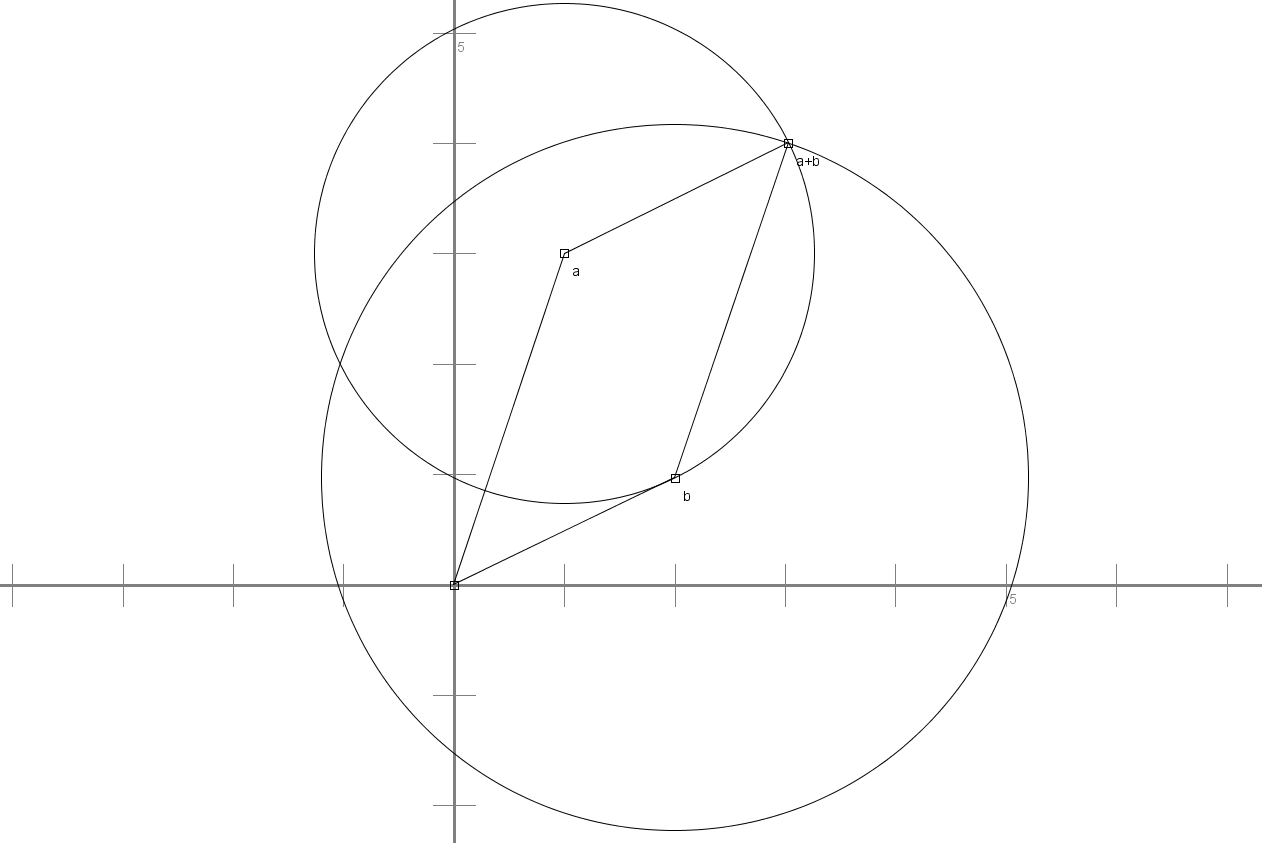
\includegraphics[width=0.6\textwidth]{alg16a1.png}
\end{center}
$-a \in K(M):$
\begin{center}
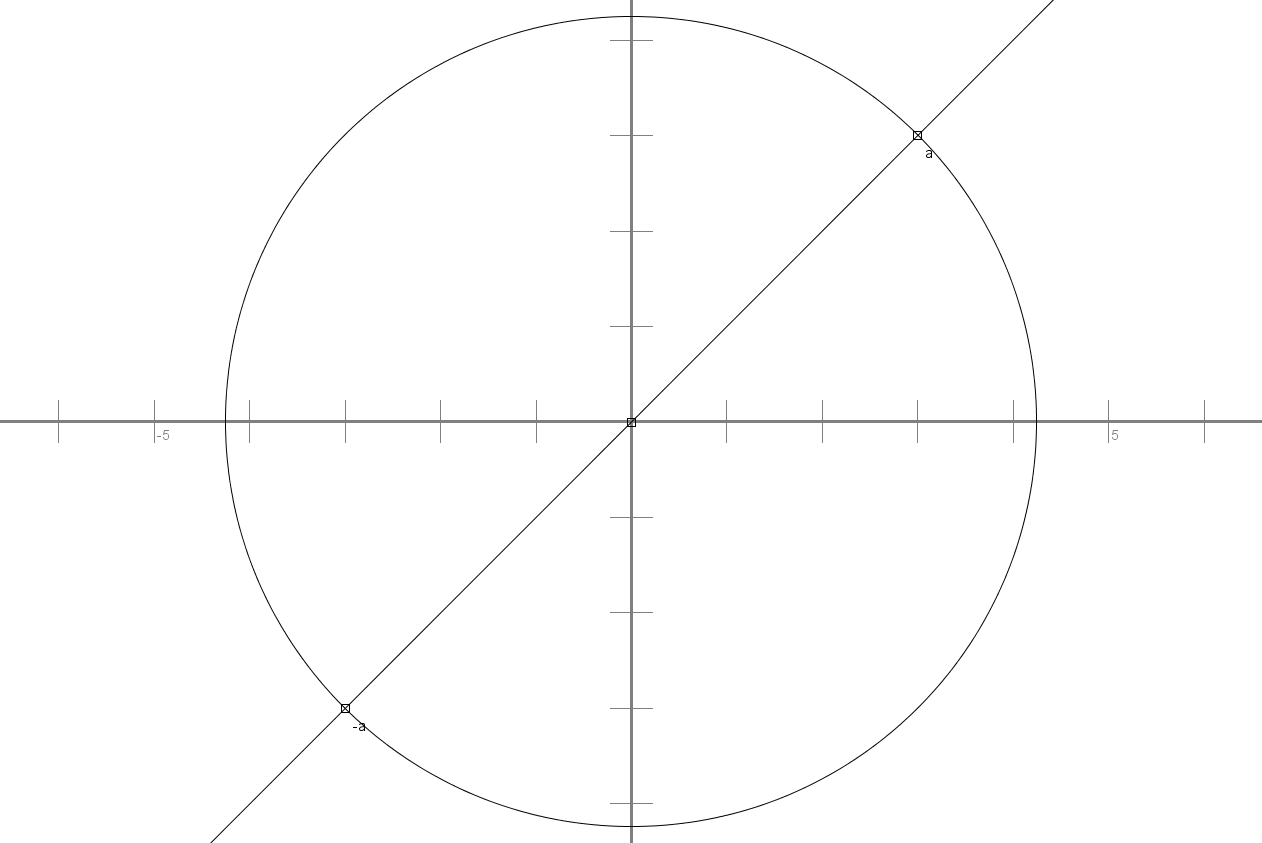
\includegraphics[width=0.6\textwidth]{alg16a2.png}
\end{center}
$a \cd b \in K(M):$\newline
Strahlensatz: $\frac{1}{a} = \frac{b}{x}$, also $x = a \cd b$. Winkel addieren
$\chk \Ra a \cd b$ allgemein $\chk$
\begin{center}
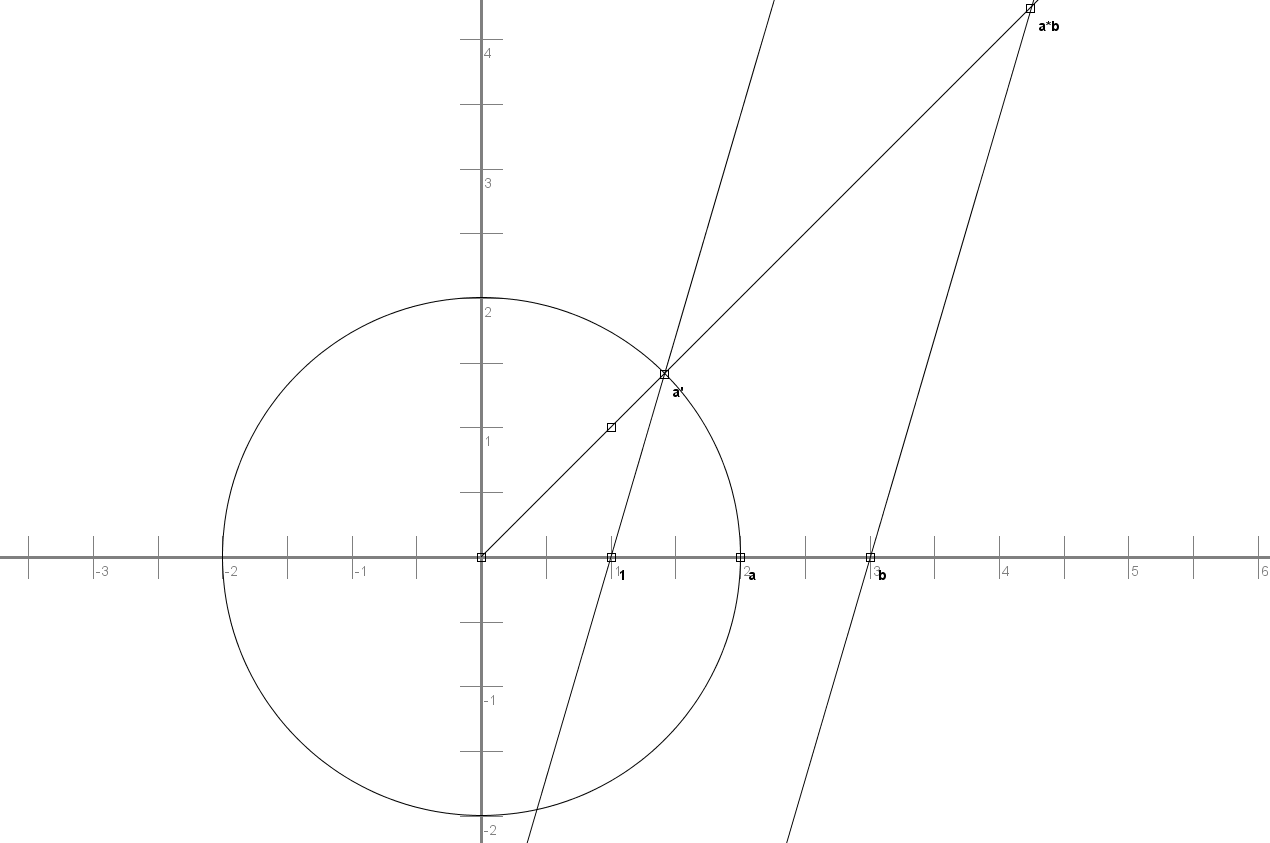
\includegraphics[width=0.6\textwidth]{alg16a3.png}
\end{center}

$\frac{1}{a} \in K(M):$ \OE $a \in \mathbb{R}$
\begin{center}
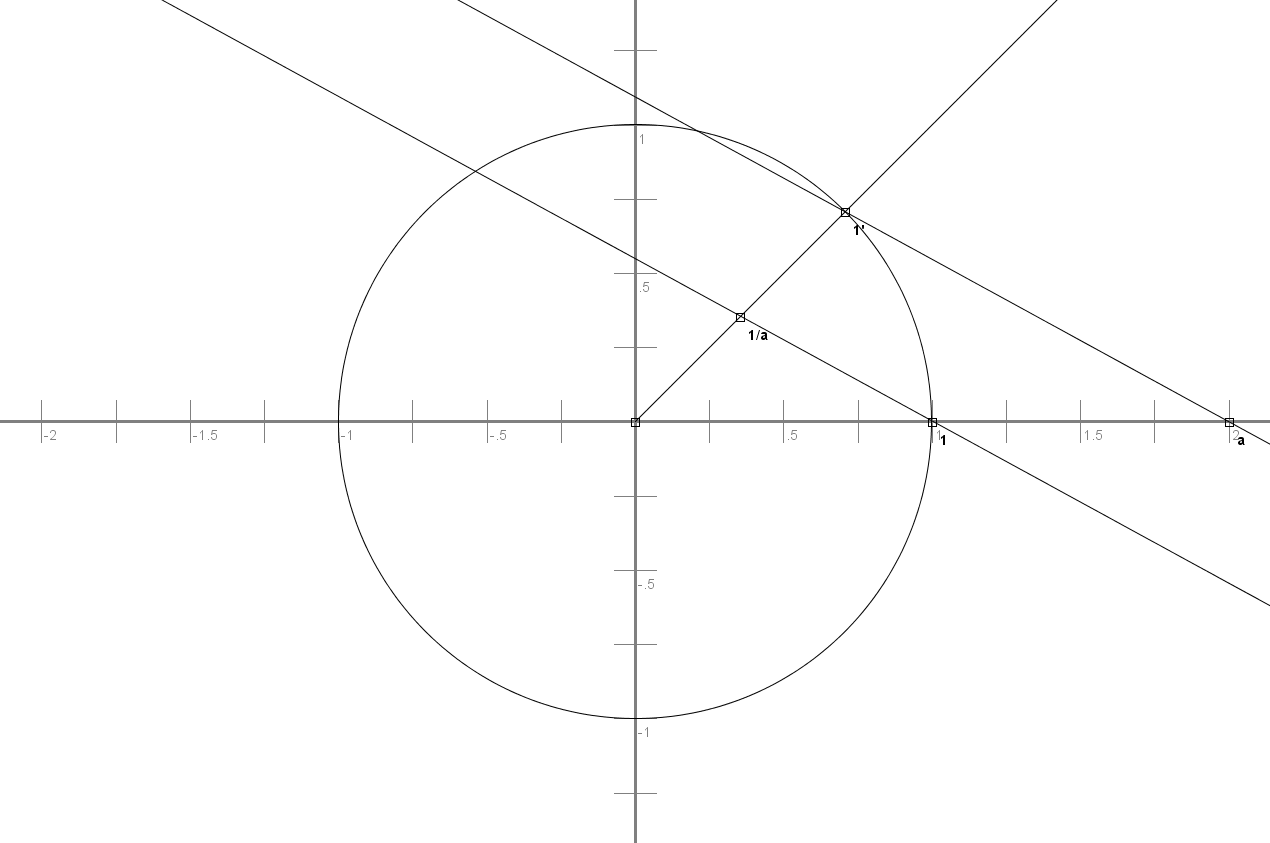
\includegraphics[width=0.6\textwidth]{alg16a4.png}
\end{center}

\item folgt aus (a)

\item Zeige mit Induktion über $n$: Jedes $a\in K_n(M)$ ist algebraisch über $\mathbb Q(M)$. Wegen $K_n(M)=K_1(\mathcal L_n(M))$ genügt es, die Behauptung für $n=1$ zu zeigen. Sei also $z\in K_1(M)$.

Vorüberlegung: Für $z \in M$ ist $\Re(z) =
\frac{1}{2}(z+\bar z) \in \mathbb{Q}(M)$ und $\Im(z) = \frac{1}{2}(z
-\bar z) \in \mathbb{Q}(M).$
\begin{enum}
\item $z$ ist Schnittpunkt zweier Geraden in $\mathcal{L}(M) \Ra
z$ ist Lösung zweier linearer Gleichungen $z_1 + \lambda z_2 = z_1'
+ \mu z_2'$
\item $z$ ist Schnittpunkt einer Geraden und eines Kreises: $\Ra$
quadratische Gleichung mit Koeffizienten in $\mathbb{Q}(M)$
\item $z$ ist Schnittpunkt zweier Kreise $K_{r_1}(m_1)$ und
$K_{r_2}(m_2)$ mit Mittelpunkten $m_1,m_2 \in M$. Radien: $r_1 =
|z_1 - z_1'|$, $r_2 = \dots$ also $r_1^2 = (z_1 - z_1') (\overline{z_1 -
z_1'}) \in \mathbb{Q}(M)$.

Dann ist $|z-m_1|^2 = r_1^2$.

$\Ra z\bar z - (z\bar{m_1} + \bar z m_1) = r_1^2 - m_1 \bar{m_1}$
und $z \bar z - (z \bar{m_2} + \bar z m_2) = r_2^2 - m_2 \bar{m_2}
\Ra 2 \Re[z(\bar{m_1} - \bar{m_2})] = r_1^2 - r_2^2 - (m_1 \bar{m_1}
- m_2 \bar{m_2})$

Das ist eine lineare Gleichung, die $\Re(z)$ und $\Im(z)$ enthält.
Einsetzen in $(1)$ ergibt quadratische Gleichung für $\Re(z)$ (mit
Koeffizienten in $\mathbb{Q}(M)$).
\end{enum}

Noch zu zeigen: Ist $a\in \mathbb C$ und gibt es eine Kette 
\[
\mathbb Q(M) = L_0\subset L_1\subset \cdots \subset L_n
\]
von Körpererweiterungen mit $[L_i:L_{i-1}]=2$ und $a\in L_n$, so ist $a\in K(M)$.

Sei also $L/K$ quadratische Erweiterung von Körpern (mit Charakteristik ungleich 2). Dann gibt es $\alpha\in L$ und $a \in K$, so dass $L=K(\alpha)$ und $\alpha^2=a$, das heißt $L=K(\sqrt{a})$. Zu zeigen ist also: Ist $K\subset K(M)$, so ist $\sqrt a\in K(M)$:

Wurzelziehen: $a \in \mathbb{R}$
\begin{center}
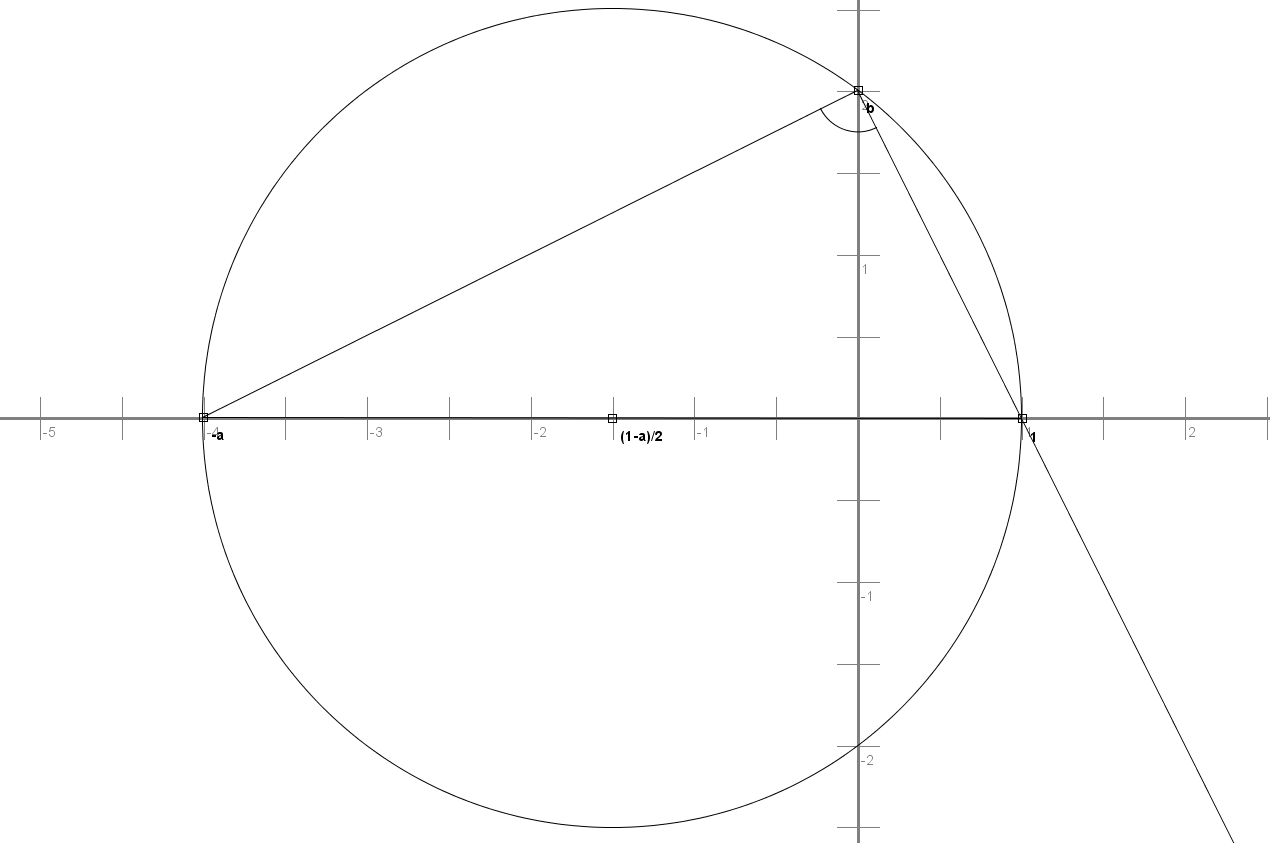
\includegraphics[width=0.6\textwidth]{alg16b.png}
\end{center}
$\overset{\scriptsize\mbox{Thales}}{\Ra}$ Winkel ist rechtwinklig
$\overset{\scriptsize\mbox{Höhensatz}}{\Ra} b^2=|-a| \cd 1 = a$
}
\end{Satz}

\bsp{
Das regelmäßige Fünfeck ist aus 0 und 1 konstruierbar. Ziel: Konstruiere Nullstellen von $X^5-1=(X-1)\cdot f$, $f\defeqr X^4+X^3+X^2+X+1$. Trick von Lagrange: $f(X) = X^2(X^2 + \frac1{X^2} + X + \frac1{X} + 1)$. Mit $Y\defeqr X+ \frac 1X$ ist dann $\frac 1{X^2} \cdot f(X) = Y^2+Y-1\defeql g(Y)$. Ist $y$ Nullstelle von $g$ und $\xi$ Nullstelle von $f$, so ist $\mathbb Q\subset \mathbb Q(y) \subset \mathbb Q(\xi)$ eine Kette wie im Satz.
}


\chapter{Galois-Theorie}

\section{Der Hauptsatz}

\begin{DefProp}
\label{4.1}
    Sei $L/K$ algebraische Körpererweiterung, $\bar K$ ein algebraischer Abschluss von $L$.

    \begin{enum}
        \item $L/K$ heißt \emp{normal}, wenn es eine Familie $\mathcal{F} 
        \subset K[X]$ gibt, so dass $L$ Zerfällungskörper von $\mathcal{F}$ ist.

        \item Ist $L/K$ normal, so ist Hom$_K(L,\bar K) =$ Aut$_K(L)$
        \sbew{
            ''$\supseteq$'' gilt immer. ''$\subseteq$'': Sei $L =
            Z(\mathcal{F})$, $f \in \mathcal{F}$, $\alpha \in L$ Nullstelle von
            $f \Ra$ Für $\sigma \in$ Hom$_K(L,\bar K)$ ist $\sigma(\alpha)$ auch
            Nullstelle von $f$. Sei $f(X) = \displaystyle \sum_{i=0}^n a_i X^i
            \Ra 0 = \sigma(f(\alpha)) = \sum_{i=0}^n 
            \underset{=a_i}{\underbrace{\sigma(a_i)}} \sigma(\alpha^i) = 
            f(\sigma(\alpha)) \Ra \sigma(\alpha) \in L \Ra \sigma(L) \subseteq L$. $\sigma$ ist surjektiv, da $L$ von den
            Nullstellen der $f \in \mathcal{F}$ erzeugt wird und jedes $f\in \mathcal F$ endlich viele Nullstellen hat, die durch $\sigma$ permutiert werden.
        }

        \item $L/K$ heißt \emp{galoissch}, wenn $L/K$ normal und separabel ist.

        \item Ist $L/K$ galoissch, so heißt \emp{Gal}$\mathbf(L/K)$ $\defeqr$
        Aut$_K(L)$ die \emp{Galoisgruppe} von $L/K$.

        \item Eine endliche Erweiterung $L/K$ ist genau dann galoissch, wenn 
        $|$Aut$_K(L)| = [L:K]$
        \sbew{''$\Ra$'' Aus (b) folgt \[|\mbox{Aut}_K(L)| = 
        |\mbox{Hom}_K(L,\bar K)| = [L:K]_s \overset{\mbox{\scriptsize
\ref{Satz 13}}}{=} [L:K] (\ast)\]

''$\Leftarrow$'' In $(\ast)$ gilt stets $|\mbox{Aut}_K(L)| \leq 
|\mbox{Hom}_K(L,\bar K)| = [L:K]_s \leq [L:K]$. Aus
$|$Aut$_K(L)| = [L:K]$ folgt also $[L:K]_s = [L:K] \Ra L/K$
separabel $\overset{\ref{Satz 14}}{\Ra} L=K(\alpha)$ für ein $\alpha
\in L$; Sei $f \in K[X]$ das Minimalpolynom von $\alpha$. Sei $\beta
\in \bar K$ Nullstelle von $f$. Nach \ref{3.8} gibt es $\sigma \in$
Hom$_K(L,\bar K)$ mit $\sigma(\alpha) = \beta$. Wegen $(\ast)$ ist
$\sigma \in$ Aut$_K(L) \Ra \beta \in L \Ra L =$ Z$(f)$. }
\end{enum}
\end{DefProp}

\bsp{
Sei $K$ Körper mit Charakteristik nicht 2, $d\in K^\times \setminus (K^\times)^2$. Dann ist $K{\sqrt{d}}/K$ eine Galois-Erweiterung, denn $X^2-d$ ist irreduzibel und separabel und zerfällt in $K(\sqrt d)[X]$ in $(X-\sqrt d)(X+ \sqrt d)$.
}

\begin{Bem}
\label{4.1.2}
\begin{enum}

\item Ist $L/K$ galoissch und $E$ ein Zwischenkörper, so ist $L/E$
galoissch und Gal$(L/E) \subseteq$ Gal$(L/K)$.

\sbew{$L/E$ normal, da Zerfällungskörper von $\mathcal{F}
\subset K[X] \subseteq E[X]$. $L/E$ separabel, da $L/K$ separabel und das Minimalpolynomm von $\alpha\in L$ über $E$ in $E[X]$ Teiler des Minimalpolynoms über $K$ ist.}

\item Ist in (a) zusätzlich auch $E/K$ galoissch, so ist \[1 \ra
\mbox{Gal}(L/E) \ra \underset{\sigma \mapsto
\sigma_{|E}}{\mbox{Gal}(L/K) \overset{\beta}{\ra} \mbox{Gal}(E/K)}
\ra 1\] exakt.

\sbew{Für $\sigma \in$ Gal$(L/K) =$ Aut$_K(L)$ ist
$\sigma_{|E}: E \ra L$, also $\sigma \in$ Hom$_K(E,L) \subseteq$
Hom$_K(E, \bar K) =$ Aut$_K(E)$, da $E/K$ galoissch ist. $\Ra \beta$
ist wohldefiniert.

$\beta$ \textbf{surjektiv}: Sei $\sigma \in$ Gal$(E/K)$. Nach
\ref{3.10} läßt sich $\sigma$ fortsetzen zu $\wt{\sigma}: L\ra \bar
K$, $\wt{\sigma} \in$ Hom$_K(L, \bar K) =$ Aut$_K(L)$ = Gal$(L/K)$
und $\beta(\wt{\sigma}) = \wt{\sigma}_{|E} = \sigma$

$\Kern \beta = \{ \sigma \in$ Gal$(L/K):\; \sigma_{|E} = id_E\} =$
Aut$_E(L) =$ Gal$(L/E)$}
\end{enum}
\end{Bem}

\begin{Satz}[Hauptsatz der Galoistheorie]
\label{Satz 17}
Sei $L/K$ endliche Galois-Erweiterung.
\begin{enum}

\item Die Zuordnungen
\[\begin{array}{ccc}
\{\mbox{Zwischenkörper von } L/K \}
&\begin{array}{c} \overset{\Psi}{\longrightarrow} \\
\underset{\Phi}{\longleftarrow}\end{array} &\{\mbox{Untergruppen von
Gal}(L/K)\} \\
E & \longmapsto & \mbox{Gal}(L/E) \\
L^H = \{\alpha \in L: \sigma(\alpha) = \alpha\; \forall \sigma \in
H\} &\longmapsfrom & H\end{array}\] sind bijektiv und zueinander
invers.

\item Ein Zwischenkörper $E$ von $L/K$ ist genau dann galoissch über
$K$, wenn Gal$(L/E)$ Normalteiler in Gal$(L/K)$ ist.
\end{enum}

\bew{}{\item $L^H$ ist Zwischenkörper: $\chk$

''$\Psi \circ \Phi = id$'': Sei $H \subseteq$ Gal$(L/K)$
Untergruppe. z.z.: Gal$(L/L^H) = H$

''$\supseteq$'' Nach Def. von $L^H$ ''$\subseteq$'': Nach \ref{4.1}
ist $|$Gal$(L/L^H)| = [L:L^H]$. Es genügt also z.z.: $[L:L^H] \leq
|H|$. Sei $\alpha \in L$ primitives Element von $L/L^H$, also
$L=L^H(\alpha)$. Sei $f \defeqr \displaystyle \prod_{\sigma \in H} (X-
\sigma(\alpha)) \in L[X]$; dann ist deg$(f) = |H|$. Für jedes $\tau
\in H$ ist $f^\tau = f$ (mit $\sigma$ durchläuft auch $\sigma \circ
\tau$ alle Elemente von $H$) $\Ra f \in L^H[X] \Ra$ Das
Minimalpolynom $g$ von $\alpha$ über $L^H$ ist Teiler von $f$. $\Ra
[L:L^H] =$ deg$(g) \leq$ deg$(f) = |H|$

''$\Phi \circ \Psi = id$'': Sei $E$ Zwischenkörper, $H \defeqr$
Gal$(L/E)$. zu zeigen: $E = L^H$.

''$\subseteq$'': Definition. ''$\supseteq$'': Da $L^H/E$ separabel
ist, genügt es zu zeigen $[L^H :E]_s = 1$. Sei also $\sigma \in$
Hom$_E(L^H,\bar K)$, $\wt{\sigma} \in$ Hom$_E(L,\bar K) =$ Aut$_E(L)
=$ Gal$(L/E)=H$ Fortsetzung $\Ra
\underset{=\sigma}{\wt{\sigma}_{|L^H}} = id_{L^H}$

\item ''$\Ra$'': \ref{4.1.2} b), da $\operatorname{Gal}(L/E)=\operatorname{Kern}\beta$.
''$\Leftarrow$'': Sei $H \defeqr$ Gal$(L/E)$ Normalteiler in
Gal$(L/K)$. Wegen \ref{4.1} c) genügt es zu zeigen: Für jedes $\sigma
\in$ Hom$_K(E,\bar K)$ ist $\sigma(E) \subseteq E$. Sei also $\sigma
\in$ Hom$_K(E,\bar K)$, $\underset{=\mbox{\scriptsize
Gal}(L/K)}{\wt{\sigma} \in\mbox{ Hom}_K(L,\bar K)}$ Fortsetzung.

Sei nun $\alpha \in E$, $\tau \in H$. Dann ist $\tau(\sigma(\alpha))
= (\tau \circ \wt{\sigma})(\alpha) =
(\wt{\sigma}\circ\tau')(\alpha)=\wt{\sigma}(\alpha) = \sigma(\alpha) $ mit $\wt{\sigma}$ wie eben und
$\tau' \defeqr \wt{\sigma}^{-1}\circ \tau \circ \wt{\sigma} \in H $
(nach Voraussetzung) $\Ra
\sigma(\alpha) \in L^H  = E\; \chk$}
\end{Satz}

\begin{Folg}
Sei $L/K$ endliche Galoiserweiterung. Dann
gilt für Zwischenkörper $E,E'$ bzw. Untergruppen $H,H'$ von
Gal$(L/K)$: \begin{enum}
\item $E \subseteq E' \iff \operatorname{Gal}(L/E) \supseteq \operatorname{Gal}(L/E')$

      $H \subseteq H' \iff L^H \supseteq L^{H'}$

\item $\operatorname{Gal}(L/E \cap E') = \langle \operatorname{Gal}(L/E), \operatorname{Gal}(L/E')\rangle$

      $E\cap E' = L^{\langle \operatorname{Gal}(L/E), \operatorname{Gal}(L/E')\rangle}$

      $L^{H\cap H'} = L^H \cdot L^{H'} \defeqr K(L^H \cup L^{H'})$ (das \emp{Kompositum} von $L^H$ und $L^{H'}$)

\end{enum}
\end{Folg}

\begin{Folg}
Zu jeder endlichen separablen
Körpererweiterung gibt es nur endlich viele Zwischenkörper.

\sbew{Ist $L/K$ endliche Galoiserweiterung, so entsprechen die
Zwischenkörper (nach \ref{Satz 17}) bijektiv den Untergruppen der
endlichen Gruppe$(L/K)$. Im allgemeinen ist $L=K(\alpha)$ (\ref{Satz 14}). Sei
$f$ das Minimalpolynom von $\alpha$ über $K$. $f$ ist separabel, da $L/K$
separabel. Sei $\wt{L}$ der Zerfällungskörper von $f$ über $K$.
$\Ra \wt{L}/K$ ist galoissch, $K \subseteq L \subseteq \wt{L} \Ra
L/K$ hat nur endlich viele Zwischenkörper. }
\end{Folg}

\begin{Prop}
\label{4.4}
Sei $L$ ein Körper, $G \subseteq$ Aut$(L)$
eine endliche Untergruppe. $K \defeqr L^G = \{\alpha \in
L:\,\sigma(\alpha) = \alpha\;\forall\; \sigma \in G\}$

Dann ist $L/K$ Galoiserweiterung und Gal$(L/K) = G$

\sbew{\begin{itemize}
\item $L/K$ ist algebraisch und separabel. Sei dazu $\alpha \in L$.
$\{\sigma(\alpha):\; \sigma \in G\} = G \alpha$  ist endlich. Sei
$G\alpha = \{\sigma_1(\alpha),\dots,\sigma_r(\alpha)\}$ mit
$\sigma_i(\alpha) \neq \sigma_j(\alpha)$ für $i\neq j$ und $\sigma_1
= id_L$. Dabei ist $r$ ein Teiler von $n := |G|$. Sei $f_\alpha(X)
\defeqr \displaystyle \prod_{i=1}^r (X- \sigma_i(\alpha)) \in L[X]$. Zu zeigen:
$f_\alpha \in K[X]$. \textbf{denn}: für $\sigma \in G$ ist
$f_\alpha^\sigma(X) = \displaystyle \prod_{i=1}^r (X -\sigma(\sigma_i(\alpha)))$
(selbe Faktoren wie $f_\alpha(X)$) $\Ra f_\alpha = f_\alpha^\sigma$
$\Ra f_\alpha \in K[X]$

$\Ra \alpha$ algebraisch, $\alpha$ separabel (da $f_\alpha$
separabel), $[K(\alpha):K] \leq n \hfill(\ast)$

\item $L/K$ normal: Der Zerfällungskörper von $f_\alpha$ ist in $L$
enthalten. $\Ra L$ ist der Zerfällungskörper der Familie
$\{f_\alpha:\;\alpha \in L\}$

\item $L/K$ endlich: Sei $(\alpha_i)_{i\in I}$ Erzeugendensystem von
$L/K$. Für jede endliche Teilmenge $I_0 \subseteq I$ ist
$K(\{\alpha_i:\;i\in I_0\})$ endlich über $K$, also
$K(\{\alpha_i:\;i\in I_0\}) = K(\alpha_0)$ für ein $\alpha_0 \in L
\overset{(\ast)}{\Ra} [K(\{\alpha_i:\;i\in I_0\}):K] \leq n$. Sei
$I_1 \subseteq I$ endlich, so dass $K_1 \defeqr K(\{\alpha_i:\;i\in
I_1\})$ maximal unter den $K(\{\alpha_j:\;j\in J\})$ für $J \subseteq I$
endlich.

\textbf{Ann.}: $K_1 \neq L$. Dann gibt es $i \in I$ mit $\alpha_i
\not \in K_1 \Ra K_1(\alpha_i) \supsetneq K_1$, trotzdem endlich im
Widerspruch zu Wahl von $K_1 \Ra L/K$ endlich, genauer $[L:K] \leq
n$ wegen $(\ast)$.

\item Gal$(L/K) = G$: ''$\supseteq$'': nach Definition. Nach
\ref{4.1} ist $n = |G| \leq |$Gal$(L/K)| = [L:K] \leq n$
\end{itemize}}
\end{Prop}


\section{Die Galoisgruppe einer Gleichung}

\begin{DefBem}
Sei $K$ ein Körper, $f \in K[X]$ ein separables Polynom.

\begin{enum}
\item Sei $L= L(f)$ Zerfällungskörper von $f$ über $K$. Dann heißt
Gal$(f) \defeqr$ Gal$(L/K)$ \empind{Galoisgruppe von $\mathbf{f}$}{Galoisgruppe
von f}.

\item Ist $n =$ deg$(f)$, so gibt es injektiven
Gruppenhomomorphismus Gal$(f) \hookrightarrow S_n$ (durch
Permutation der Nullstellen von $f$)

\item Ist $L/K$ separable Körpererweiterung vom Grad $n$, so ist
Aut$_K(L)$ isomorph zu einer Untergruppe von $S_n$.

\sbew{Sei $L=K(\alpha)$, $f \in K[X]$ Minimalpolynom
von $\alpha$, $\alpha= \alpha_1,\dots,\alpha_d$ die Nullstellen von
$f$ in $L \Ra$ jedes $\sigma \in$ Aut$_K(L)$ permutiert
$\alpha_1,\dots,\alpha_d$.}
\end{enum}
\end{DefBem}

\begin{Bspe}
Die Galoisgruppe von $f(X) = X^5 - 4X + 2 \in
\mathbb{Q}[X]$ ist $S_5$.
\newline\newline\textbf{Bew.}:\begin{itemize}

\item $f$ ist irreduzibel: Eisenstein für $p=2$

\item $f$ hat 3 relle und 2 zueinander konjugiert komplexe
Nullstellen $f(-\infty) = -\infty,\;f(0)=2,f(1) =
-1,f(\infty)=\infty$ $\Ra f$ hat mindestens $3$ reelle Nullstellen.

$f'(X) = 5X^4 - 4 = 5(X^2 - \frac{2}{\sqrt{5}})(X^2 +
\frac{2}{\sqrt{5}})$ hat $2$ reelle Nullstellen $\Ra f$ hat genau
$3$ reelle Nullstellen. Ist $\alpha \in \mathbb{C}$ Nullstelle von
$f$, so ist $f(\bar \alpha) = \overline{f(\alpha)} = 0$.

\item $G=$ Gal$(f)$ enthält die komplexe Konjugation $\tau$. $\tau$
operiert als Transposition: $2$ Nullstellen werden vertauscht, $3$
bleiben fix.

\item $G$ enthält ein Element von Ordnung $5$: Ist $\alpha$
Nullstelle von $f$, so ist $[\mathbb{Q}(\alpha):\mathbb{Q}] = 5$ und
$\mathbb{Q}(\alpha) \subseteq L(f) \overset{\ref{Satz 17}}{\Ra} 5$
teilt $|G| \overset{\mbox{\scriptsize Sylow}}{\Ra}$ Beh.

\item $G$ enthält also einen $5$-Zyklus und eine Transposition
$\overset{\mbox{(!)}}{\Ra} G = S_5$.
\end{itemize}
\end{Bspe}

\begin{Bem}
Allgemeine Gleichung $n$-ten Grades: Sei $k$
ein Körper, $L = k(T_1,\dots,T_n) =$ Quot$(k[T_1,\dots,T_n])$

\begin{itemize}
\item $S_n$ operiert auf $L$ durch $\sigma(T_i) = T_{\sigma(i)}$

\item Sei $K\defeqr L^{S_n}$. $L/K$ ist Galois-Erweiterung (nach
Proposition \ref{4.4}) vom Grad $n!$

\item $L$ ist (über $K$) Zerfällungskörper von $f(X) =
\displaystyle \prod_{i=1}^n(X-T_i) \in K[X]$

\item Gal$(f) = S_n$

\item $f(X) = \displaystyle \sum_{\nu = 0}^n (-1)^{\nu} s_{\nu}
(T_1,\dots,T_n)X^{n-\nu}$ mit $s_{\nu}(T_1,\dots,T_n) =
\displaystyle \sum_{1\leq i_1 < \dots < i_{\nu} \leq n} T_{i_1} \cd \dots \cd 
T_{i_\nu}$

z.B.: $s_1(T_1,\dots,T_n) = T_1 + \dots + T_n$, $s_2 = T_1 T_2 + T_1
T_3 + \dots + T_{n-1}T_n$, $s_n = T_1 \cd \dots \cd T_n$

\item $K = k(s_1,\dots,s_n)$
\end{itemize}
\end{Bem}
\section{Einheitswurzeln}

\begin{BemDef}
\label{4.8}
Sei $K$ ein Körper, $\bar K$
algebraischer Abschluss von $K$, $n \in\mathbb{N}$ teilerfremd zu char$(K)$.

\begin{enum}
\item Die Nullstellen von $X^n - 1$ in $\bar K$ heißen
$\mathbf{n}$\emp{-te Einheitswurzeln}.

\item $\mu_n(\bar K) \defeqr \{\zeta \in \bar K: \zeta^n = 1\}$ ist
zyklische Untergruppe von ${\bar K}^x$ der Ordnung $n$.

\sbew{$\mu_n(\bar K)$ Untergruppe $\checkmark$, also zyklisch
nach \ref{3.17}. $f(X) = X^n-1$ ist separabel, da $f'(X) = nX^{n-1}$
(Bem \ref{3.13})}

\item Eine $n$-te Einheitswurzel $\zeta$ heißt \emp{primitiv}, wenn
$\langle \zeta \rangle = \mu_n(\bar K)$
\end{enum}
\end{BemDef}

\begin{Satz}
(Voraussetzungen wie eben), $n \geq 2$
\begin{enum}
\item Die Anzahl der primitiven Einheitswurzeln in $\bar K$ ist
$\varphi(n) = |(\mathbb{Z}/n\mathbb{Z})^x| = \{ m\in \{1,\dots,n\} :
$ggT$(m,n) = 1\}$ ($n \mapsto \varphi(n)$ ist Eulersche
$\varphi$-Funktion)

\sbew{Ist $\zeta$ primitive $n$-te Einheitswurzel, so ist
$\mu_n(\bar K) = \{1,\zeta, \zeta^2, \dots, \zeta^{n-1}\}$, $\zeta^k$
erzeugt $\{1,\zeta, \zeta^2, \dots, \zeta^{n-1}\} \lra$ ggT$(n,k) = 1$.}

\item Ist $n = p_1^{\nu_1} \dots p_r^{\nu_r}$,
(Primfaktorzerlegung) so ist $\varphi(n) = \displaystyle \prod_{i=1}^r
p_i^{\nu_i-1} (p_i - 1)$

\sbew{$\mathbb{Z}/n\mathbb{Z} =
\mathbb{Z}/p_1^{\nu_1}\mathbb{Z} \bigoplus \dots \bigoplus
\mathbb{Z}/p_r^{\nu_r} \mathbb{Z}$ (Satz \ref{Satz 8}) $\Ra
(\mathbb{Z}/n\mathbb{Z})^x  = (\mathbb{Z}/p_1^{\nu_1} \mathbb{Z})^x
\bigoplus \dots \bigoplus (\mathbb{Z}/p_r^{\nu_r} \mathbb{Z})^x$

$|(\mathbb{Z}/p^\nu \mathbb{Z})^x| = p^{\nu} - p^{\nu-1} = p^{\nu -
1}(p-1)$}

\item Sind $\zeta_1,\dots,\zeta_{\varphi(n)}$ die primitiven
Einheitswurzeln, so heißt $\Phi_n(X) \defeqr
\displaystyle \prod_{i=1}^{\varphi(n)} (X- \zeta_i) \in \bar K[X]$ das $n$-te
\emp{Kreisteilungspolynom}

\item $X^n - 1 = \displaystyle \prod_{d \mid n} \Phi_d(X)$

\sbew{$X^n - 1 = \displaystyle \prod_{\zeta \in \mu_n} (X-\zeta) =
\prod_{d \mid n} \prod_{\substack{\zeta \in \mu_n \\ ord(\zeta) = d}} (X-\zeta) = \prod_{d
\mid n} \Phi_d(X)$}

\item Sei $\zeta$ primitive $n$-te Einheitswurzel. Dann ist
$K(\zeta)/K$ Galois-Erweiterung.
\sbew{$K(\zeta)$ ist
Zerfällungskörper von $X^n - 1$ über $K$, also normal. $X^n - 1$ ist
separabel (\ref{4.8})}

\item \[\chi_n: \begin{array}{ccc} \mbox{Gal}(K(\zeta)/K) &\ra
&(\mathbb{Z}/n\mathbb{Z})^x \\ \sigma &\mapsto &\chi_n(\sigma)
\end{array}\] ist injektiver Gruppenhomomorphismus, wobei
\newline $\sigma(\zeta) = \zeta^{\chi_n(\sigma)}$. ($\chi_n$ heißt
\emp{zyklotomischer Charakter})

\sbew{$\chi_n(\sigma) \in (\mathbb{Z}/n\mathbb{Z})^x$, da
$\sigma(\zeta)$ primitive Einheitswurzel sein muß.

$\chi_n$ ist Gruppenhomomorphismus: $\sigma_1, \sigma_2 \in$
Gal$(K(\zeta)/K) \Ra \sigma_1(\sigma_2(\zeta)) =
\sigma_1(\zeta^{\chi_n(\sigma_2)}) =
(\sigma_1(\zeta))^{\chi_n(\sigma_2)} = \zeta^{\chi_n(\sigma_1)
\chi_n(\sigma_2)}$

$\chi_n$ injektiv: $\chi_n(\sigma) = 1 \Ra \sigma(\zeta) = \zeta \Ra
\sigma = id$}

\item $\Phi_n(X) \in K[X]$, genauer $\Phi_n(X) \in \left\{
\begin{array}{ll} \mathbb{Z}[X] \mbox{ (primitiv) } &:\mbox{char}(K) =
0 \\ \mathbb{F}_p[X] &:\mbox{char}(K) = p \end{array}\right.$
\newline
\sbew{
Induktion über $n$: $n=2\;\checkmark$

$n>2$: $\underset{(\ast)}{\underbrace{X^n - 1}} \overset{(d)}{=} \Phi_n(X)
\underset{ (\ast \ast)}{\underbrace{\displaystyle \prod_{\substack{d \mid n\\
d < n}} \Phi_d(X)}}$

char$(K) = p : (\ast) \in \mathbb{F}_p[X]$, $(\ast \ast) \in \mathbb{F}_p[X]
\mbox{ nach IV} \Ra \Phi_n(X) \in \mathbb{F}_p[X]:$ Eukl. Alg.

char$(K) = 0: (\ast) \in \mathbb{Z}[X]$ (primitiv), $(\ast \ast) \in
\mathbb{Z}[X]$ primitiv nach IV

% TODO Lemma von Gauß = Satz von Gauß = Satz 11???
$\overset{\mbox{\scriptsize Lemma von Gauß}}{\Ra} \Phi_n(X) \in
\mathbb{Z}[X]$ primitiv.
}

\item Ist $K = \mathbb{Q}$, so ist $\Phi_n$ irreduzibel und $\chi_n$
ein Isomorphismus. $\mathbb{Q}(\zeta)$ heißt $n$-ter
\emp{Kreisteilungskörper}.

\sbew{
Es genügt zu zeigen: $\Phi_n$ irreduzibel (dann folgt $\chi_n$
Isomorphismus aus (e) und (f))

Sei $f \in \mathbb{Q}[X]$ Minimalpolynom von $\zeta$, $f \in
\mathbb{Z}[X]$ wegen (g)

\textbf{Beh.}: $f(\zeta^p) = 0$ für jede Primzahl $p$ mit $p \nmid
n$. Dann ist auch $f(\zeta^m) = 0$ für jedes $m$ mit ggT$(m,n) = 1\Ra
f(\zeta_i) = 0$ für jede primitive Einheitswurzel $\zeta_i \Ra
\Phi_n|f \Ra \Phi_n = f$

\textbf{Bew.}: Sei $X^n - 1 = f \cd h$. Wäre $f(\zeta^p) \neq 0 \Ra
h(\zeta^p) = 0$ dh. $\zeta$ Nullstelle von $h(X^p) \Ra h(X^p)$ ist
Vielfaches von $f \Ra \exists\;g \in \mathbb{Z}[X]$ mit $h(X^p) = f
\cd g\\ \overset{mod\;p}{\Ra} \bar f \bar g = {\bar h}^p$ in $\bar
{\mathbb{F}}_p [X] \Ra \bar f$ und $\bar h$ haben gemeinsame
Nullstellen in $\bar {\mathbb{F}}_p \Ra X^n - \bar 1 = \bar f \bar
h$ hat doppelte Nullstelle $\blitzb$ zu $X^n - 1$ separabel.
}
\end{enum}

\textbf{\newline Beispiele:} $\ds\Phi_2(X) = X+1$, $\Phi_p(X) =
X^{p-1} + X^{p-2} + \dots + X + 1$

\[\Phi_4(X) = \frac{X^4-1}{\Phi_2 \cd \Phi_1} = \frac{X^4-1}{X^2 -1} =
X^2 + 1\]

\[\ds\Phi_6(X) = \frac{X^6-1}{\Phi_3 \Phi_2 \Phi_1} = \dots = X^2 - X
+ 1\]

\[\ds\Phi_8(X) = X^4 +1\] \newline\newline Für $n < 105$ sind alle
Koeffizienten $0,1$ oder $-1$.
\end{Satz}

\begin{Folg}
Das regelmäßige $n$-Eck ist genau dann mit
Zirkel und Lineal (aus $\{0,1\}$) konstruierbar, wenn $\varphi(n)$ eine Potenz von
$2$ ist.
\sbew{z.z.: $\zeta_n$ (primitive
$n$-te Einheitswurzel) $\in K(\{0,1\}) \lra \varphi(n) = 2^l$ für
ein $l \geq 1\; \lra
\underset{\varphi(n)}{\underbrace{[\mathbb{Q}(\zeta_n) :
\mathbb{Q}]}} = 2^l$ und es gibt Kette $\mathbb{Q}(M) = L_0 \subset L_1
\subset \dots \subset L_n = \mathbb{Q}(\zeta_n)$ und $[L_i :
L_{i-1}] = 2$.

''$\Leftarrow$'': Gal$(\mathbb{Q}(\zeta_n):\mathbb{Q})$ ist abelsch
von Ordnung $2^l$. Dazu gehört Kompositionsreihe mit Faktoren
$\mathbb{Z}/2\mathbb{Z} \overset{\mbox{\scriptsize Hauptsatz d.
Galoistheorie}}{\Ra}$}
\end{Folg}
\section{Norm, Spur und Charaktere}

\begin{DefProp}
\label{4.10}
Sei $G$ eine Gruppe, $K$
ein Körper.
\begin{enum}
\item  Ein \emp{Charakter} von $G$ (mit Werten in $K$) ist ein
Gruppenhomomorphismus $\chi: G\ra K^x$

\item $X_K(G) \defeqr \{ \chi: G \ra K^x,\; \chi$ Charakter$\} =$
Hom$(G,K^x)$ heißt \emp{Charaktergruppe} von $G$ (mit Werten in
$K$)

\item (Lineare Unabhängigkeit der Charaktere, E.Artin)
$X_K(G)$ ist linear unabhängige Teilmenge des $K$-Vektorraums
Abb$(G,K)$


\sbew{Angenommen $X_K(G)$ ist linear abhängig. Dann sei
$n > 0$ minimal, so dass es in $X_K(G)$ $n$ paarweise verschieden
linear abhängige Elemente gibt. Es gebe also $\chi_1,\dots,\chi_n
\in X_K(G)$, $\lambda_1,\dots,\lambda_n \in K^x$ mit $\displaystyle \sum_{i=1}^n
\lambda_i \chi_i = 0$. Dazu muß $n\geq 2$ sein.

Sei $g \in G$ mit $\chi_1(g) \neq \chi_2(g)$. Dann gilt für alle
$\ds h \in G$: \[0 = \sum_{i=0}^n \lambda_i \chi_i(gh) =
\sum_{i=1}^n \underset{\defeql \mu_i \in K^x}{\underbrace{\lambda_i \chi_i
(g)}} \chi_i(h) = \sum_{i=1}^n \mu_i \chi_i(h) \Ra \sum_{i=1}^n \mu_i
\chi_i = 0\]

Sei $\nu_i \defeqr \mu_i - \lambda_i \chi_1(g),\;i=1,\dots,n$. Dann ist
$\displaystyle \sum_{i=1}^n \nu_i\chi_i = 0,\; \nu_1 = \lambda_1 \chi_1(g)
-\lambda_1\chi_1(g)=0$, $\nu_2 = \lambda_2 \chi_2(g) - \lambda_2
\chi_1(g) = \lambda_2(\chi_2(g) - \chi_1(g)) \neq 0$ Widerspruch zur
Minimalität von $n$.}
\end{enum}
\end{DefProp}

\begin{DefBem}
Sei $L/K$ endliche
Körpererweiterung, $q\defeqr \frac{[L:K]}{[L:K]_s}$ ($=p^r,\;p=$char$(K)$), $n
\defeqr [L:K]_s$, Hom$_K(L,\bar K) = \{\sigma_1,\dots,\sigma_n\}$

\begin{enum}
\item Für $\alpha \in L$ heißt tr$_{L/K}(\alpha) \defeqr q \cd
\displaystyle \sum_{i=1}^n \sigma_i (\alpha) \in \bar K$ die \emp{Spur} von
$\alpha$ (über $K$)

\item $\forall \alpha \in L:$ tr$_{L/K}(\alpha) \in K$

\sbew{\OE $L/K$ separabel. Ist $L/K$ normal, also
galoissch, so ist Hom$_K(L,\bar K) =$ Gal$(L/K) \defeql G$ und
tr$_{L/K}(\alpha) \in L^G = K$ (da invariant unter allen $\sigma_i$). Andernfalls sei
$\wt{L}$ normale Erweiterung von
$K$ mit $L \subset \wt{L}$. Für $\tau \in$ Hom$_K(\wt{L},\bar K) =$
Gal$(\wt{L}/K)$ und jedes $i=1,\dots,n$ ist $\tau \circ \sigma_i
\in$ Hom$_K(L,\bar K)$ (da $\sigma_i(L) \subseteq \wt{L}$) $\Ra$
tr$_{L/K}(\alpha) \in {\wt{L}}^{\scriptsize\mbox{Gal}(\wt{L}/K)} = K$ }

\item tr$_{L/K}$ ist $K$-linear.

\item Für $\alpha \in L$ heißt $\ds N_{L/K}(\alpha) =
\left(\prod_{i=1}^n \sigma_i(\alpha)\right)^q$ die \emp{Norm} von
$\alpha$ (über $K$).

\item $N_{L/K}(\alpha) \in K$

\item $N_{L/K}: L^x \ra K^x$ ist Gruppenhomomorphismus

\sbew{\begin{enum}
\item[(e)] Ist $L/K$ separabel, so
argumentiere wie in (b). Sonst siehe Bosch.
\end{enum}
}
\end{enum}
\end{DefBem}

\begin{Bem}
Sei $L/K$ endliche Körpererweiterung. Für
$\alpha \in L$ sei $m_\alpha: L \ra L,\;x\mapsto \alpha x$.
$m_\alpha$ ist $K$-linear und es gilt:
\[\mbox{tr}_{L/K}(\alpha) = \mbox{Spur}(m_\alpha),\;N_{L/K}(\alpha)
= \mbox{det}(m_\alpha)\]

\sbew{Ist $L/K$ separabel, so sei $L=K(\alpha)$. Dann ist
$1,\alpha,\alpha^2,\dots,\alpha^{n-1}$ eine $K$-Basis von $L$,
$[L:K] = n$. Weiter sei $f(X) = X^n + c_{n-1} X^{n-1} + \dots + c_1
X + c_0\;\in K[X]$ das Minimalpolynom von $\alpha$ über $K$. Dann
ist die Abbildungsmatrix von $m_\alpha$ bezüglich der Basis
$1,\dots,\alpha^{n-1}$

\[ D = \begin{pmatrix}
0 & 0 &\dots & 0 & -c_0 \\
1 & 0 &      & \vdots & -c_1 \\
0 & 1 &      & \vdots & \vdots   \\
\vdots & \vdots & \ddots & 0 & \vdots \\
0 & 0 & \dots 0 & 1 & -c_{n-1}
\end{pmatrix}\]

$\Ra$ Spur$(m_\alpha) = -c_{n-1}$, det$(m_\alpha) = (-1)^n c_0$.

In $\bar K[X]$ zerfällt $f$ in Linearfaktoren:

$f = \prod_{i=1}^n(X-\sigma_i(\alpha)) \Ra c_{n-1} = \sum_{i=1}^n
\sigma_i(\alpha)$, $c_0 = (-1)^n \prod_{i=1}^n \sigma_i(\alpha)$

Ist $L\neq K(\alpha)$, so sei $b_1,\dots,b_n$ eine $K(\alpha)$-Basis
von $L$. Dann ist $B = \{ b_i
\alpha^j,\;i=1,\dots,m,\;j=0,\dots,n-1\}$ eine $K$-Basis von $L$.
Dann ist die Darstellungsmatrix von $m_\alpha$ bezüglich $B$:

\[ \wt{D} = \begin{pmatrix}
D & 0 & \dots & 0\\
0 & D & & \\
  &   & \ddots & \\
0 & 0 & & D \end{pmatrix} \] $\Ra$ Spur$(m_\alpha) = m(-c_{n-1})$,
det$(m_\alpha) = \left((-1)^n c_0 \right)^m$

Für jedes $\sigma_i \in$ Hom$_K(L,\bar K)$ ist $\sigma_i(\alpha)$
Nullstelle von $f$. Jede Nullstelle von $f$ wird dabei gleichoft
angenommen, nämlich $m = [L : K(\alpha)]$-mal $\Ra$
tr$_{L/K}(\alpha) = m \cd$ tr$_{K(\alpha)/K}(\alpha) = m(-c_{n-1})$
und $N_{L/K}(\alpha) = \left(N_{K(\alpha)/K}\right)^m = \left((-1)^n c_0 \right)^m$}
\end{Bem}

\begin{Satz}[''Hilbert(s Satz) 90'']
\label{Satz 19}
Sei $L/K$ zyklische
Galois-Erweiterung. (dh. Gal$(L/K) = \langle \sigma \rangle$ für ein
$\sigma$)
\begin{enum}

\item Ist $\beta \in L$ mit $N_{L/K}(\beta) = 1$, so gibt es ein
$\alpha \in L^x$ mit $\beta = \frac{\alpha}{\sigma(\alpha)}$

\sbew{ $n \defeqr [L:K]$. Nach \ref{4.10} sind die Charaktere
$id, \sigma,\dots,\sigma^{n-1}:\; L^x \ra L^x$ linear unabhängig
über $L$.

Nun ist $f = id + \beta \sigma + \beta\sigma(\beta) \sigma^2 + \dots
+ \beta \sigma(\beta) \dots \sigma^{n-2}(\beta) \sigma^{n-1}$
nicht die Nullabbildung $\Ra \exists \gamma \in L$ mit $\alpha
\defeqr f(\gamma) \neq 0$

$\beta \sigma(\alpha) = \beta \sigma(\gamma) + \beta \sigma(\beta)
\sigma^2 (\gamma) + \dots + \underset{N_{L/K}(\beta) =
1}{\underbrace{\beta \sigma(\beta) \dots \sigma^{n-1}(\beta)}}
\underset{=\gamma}{\underbrace{\sigma^n(\gamma)}} = \alpha$ }

\item Sei $L/K$ zyklische Galoiserweiterung, $n = [L:K]$, $\sigma \in$ Gal$(L/K)$
ein Erzeuger. Zu $\beta \in L$ mit tr$_{L/K}(\beta) = 0$ gibt es $\alpha
\in L$ mit $\beta = \alpha - \sigma(\alpha)$

\sbew{Sei $\gamma \in L$ mit tr$_{L/K}(\gamma) \neq 0$ und $\\\alpha
\defeqr \frac{1}{\mbox{\small tr}_{L/K}(\gamma)} \cd [ \beta \sigma(\gamma) +
(\beta + \sigma(\beta))\sigma^2(\gamma) + \dots + (\beta +
\sigma(\beta) + \dots + \sigma^{n-2}(\beta))\sigma^{n-1}(\gamma)]$
$\\\Ra \sigma(\alpha) = \frac{1}{\mbox{\small
tr}_{L/K}(\gamma)}[\sigma(\beta)\sigma^2(\gamma) +(\sigma(\beta) +
\sigma^2(\beta))\sigma^3(\gamma)+\dots+(\sigma(\beta) + \dots +
\sigma^{n-1}(\beta))\sigma^n(\gamma)]$ $\\\Ra (\alpha -
\sigma(\alpha))\mbox{tr}_{L/K}(\gamma) = \beta\sigma(\gamma) + \beta
\sigma^2(\gamma) + \dots + \beta\sigma^{n-1}(\gamma) -
\underset{-\beta}{\underbrace{(\sigma(\beta)+\dots+\sigma^{n-1}(\beta))}}
\gamma = \beta \cd \mbox{tr}_{L/K}(\gamma)$}
\end{enum}
\end{Satz}

\begin{Folg}
Voraussetzungen wie in Satz \ref{Satz 19}.
\begin{enum}

\item Ist char$(K)$ kein Teiler von $n=[L:K]$ und enthält $K$ eine
primitive $n$-te Einheitswurzel $\zeta$, so gibt es ein primitives
Element $\alpha \in L$, so dass das Minimalpolynom von $\alpha$ über
$K$ \[X^n - \gamma\] ist für ein $\gamma \in K$.
(\textit{''Kummer-Erweiterung''})

\item Ist char$(K) = [L:K] = p$, so gibt es ein primitives Element
$\alpha \in L$, so dass das Minimalpolynom von $\alpha$ über $K$
\[ X^p - X - \gamma\] für ein $\gamma \in K$.
(\textit{''Artin-Schreier-Erweiterung''})

\end{enum}
\bew{}{\item Es ist $N_{L/K}(\zeta) = \zeta^n = 1 =
N_{L/K}(\zeta^{-1}) \overset{\mbox{\scriptsize Satz \ref{Satz
19}}}{\Ra}$ es gibt $\alpha \in L$ mit $\sigma(\alpha) = \zeta
\alpha \Ra \sigma^i(\alpha) = \zeta^i \alpha,\;i=1,\dots,n-1$ $\Ra$
Das Minimalpolynom von $\alpha$ über $K$ hat $n$ verschiedene
Nullstellen $\Ra L = K(\alpha)$.

Außerdem ist $\sigma(\alpha^n) = \sigma(\alpha)^n = \alpha^n \Ra
\gamma \defeqr \alpha^n \in K$ $\Ra$ Das Minimalpolynom von $\alpha$
ist $X^n - \gamma$

\item tr$_{L/K}(1) = 1 + \dots + 1 = p = 0
\overset{\scriptsize\ref{Satz 19}}{\Ra}$ es gibt $\alpha \in L$ mit
$\sigma(\alpha) = \alpha + 1 \Ra \sigma^i(\alpha) = \alpha +
i,\;i=0,\dots,n-1 \Ra K(\alpha) = L$

$\sigma(\alpha^p - \alpha) = \sigma(\alpha)^p - \sigma(\alpha) =
\alpha^p + 1 - (\alpha + 1) = \alpha^p - \alpha \Ra \alpha^p -
\alpha \defeql \gamma \in K$ und $X^p -X - \gamma$ ist
Minimalpolynom von $\alpha$.}
\end{Folg}

\begin{Prop}
Sei $L/K$ einfache Körpererweiterung, $L =
K(\alpha)$

\begin{enum}

\item Ist $\alpha$ Nullstelle eines Polynoms $X^n - \gamma$ für ein
$\gamma \in K$ und enthält $K$ eine primitive $n$-te Einheitswurzel
$\zeta$, so ist $L/K$ galoissch, Gal$(L/K)$ zyklisch, $d\defeqr
[L:K]$ ist Teiler von $n$, $\alpha^d \in K$, $X^d - \alpha^d$ ist
Minimalpolynom von $\alpha$

\item Ist char$(K) = p > 0$ und $\alpha \in L\setminus K$ Nullstelle
eines Polynoms $X^p - X - \gamma$ für ein $\gamma \in K$, so ist
$L/K$ galoissch und Gal$(L/K) \cong \mathbb{Z}/p\mathbb{Z}$

\end{enum}

\bew{}{\item Die Nullstellen von $X^n - \gamma$ sind
$\alpha,\zeta\alpha,\dots,\zeta^{n-1}\alpha \Ra L$ ist
Zerfällungskörper von $X^n - \gamma$, also normal und separabel,
also galoissch.

Für $\sigma \in$ Gal$(L/K)$ ist $\sigma(\alpha) =
\zeta^{\nu(\sigma)} \alpha$ für ein $\nu(\sigma) \in
\mathbb{Z}/n\mathbb{Z}$.

$\sigma \mapsto \nu(\sigma)$ ist injektiver Gruppenhomomorphismus
Gal$(L/K) \ra \mathbb{Z}/n\mathbb{Z} \Ra$ Gal$(L/K)$ ist zyklisch,
da Untergruppe von $\mathbb{Z}/n\mathbb{Z} \Ra d = [L:K]$ teilt $n$.

Für $\sigma \in$ Gal$(L/K)$ ist $\sigma(\alpha^d) =
\left(\zeta^{\nu(\sigma)}\right)^d \alpha^d = \alpha^d \Ra \alpha^d
\in K$; $X^d - \alpha^d$ ist Minimalpolynom, da $L=K(\alpha)$ und
$[K(\alpha):K] = d$.

\item Für $i \in \mathbb{F}_p$ ist $(\alpha+i)^p - (\alpha + i) -
\gamma = \alpha^p + \underset{=i}{\underbrace{i^p}} - \alpha - i -
\gamma = 0 \Ra X^p - X - \gamma$ hat $p$ verschieden Nullstellen
$\Ra L$ ist Zerfällungskörper von $X^p - X - \gamma$ und $L/K$ ist
separabel. Außerdem folgt: Gal$(L/K) \cong \mathbb{Z}/p\mathbb{Z}$ }
\end{Prop}
\section{Auflösung von Gleichungen durch Radikale}

\begin{Def}
Sei $K$ ein Körper.
\begin{enum}

\item Eine einfache Körpererweiterung $L=K(\alpha)$ heißt
\emp{elementare (oder einfache) Radikalerweiterung}, wenn entweder

\begin{enumerate}
\item[(i)] $\alpha$ ist eine Einheitswurzel.
\item[(ii)] $\alpha$ ist Nullstelle von $X^n - \gamma$ für ein
$\gamma \in K$ und char$(K) \nmid n$
\item[(iii)] $\alpha$ ist Nullstelle von $X^p - X - \gamma$ für
$\gamma \in K$, char$(K) = p$
\end{enumerate}

\item Eine endliche Körpererweiterung $L/K$ heißt
\emp{Radikalerweiterung}, wenn es eine Körpererweiterung $L'/L$ gibt
und eine Kette $K=L_0 \subset L_1 \subset \dots \subset L_n = L'$
von Zwischenkörpern, so dass $L_{i+1}/L_i$ elementare
Radikalerweiterung ist für $i=0,\dots,n-1$

\item Ist $f \in K[X]$ separabel, nicht konstant, so heißt die
Gleichung $f(X) = 0$ \emp{durch Radikale auflösbar}, wenn der
Zerfällungskörper von $f$ Radikalerweiterung ist.
\end{enum}

\bsp{$K=\mathbb{Q}$, $f(X) = X^3 - 3X + 1$

\textbf{Beh.}: Ist $\alpha$ Nullstelle von $f$, so ist
$\mathbb{Q}(\alpha)$ Zerfällungskörper von $f$, hat also Grad $3$
über $\mathbb{Q}$. $\mathbb{Q}(\alpha)/\mathbb{Q}$ ist
\textbf{keine} einfache Radikalerweiterung.

Die Nullstellen von $f$ sind: \[\ds\begin{array}{l}\alpha_1 =
e^{2\pi i/9} + e^{16\pi i / 9} \\ \alpha_2 = e^{8\pi i/9} + e^{10
\pi i/9}
\\ \alpha_3 = e^{14 \pi i / 9} + e^{4\pi i /9} \end{array}\]

Es ist $\alpha_1^2 = e^{4\pi i /9} + e^{14 \pi i/9} + 2 = \alpha_3+2
\Ra \alpha_3 \in \mathbb{Q}(\alpha_1) \Ra \alpha_2 = -\alpha_1 -
\alpha_3 \in \mathbb{Q}(\alpha_1)$}
\end{Def}

\begin{Satz}
Sei $K$ ein Körper, $f \in K[X]$ separabel, nicht konstant.
\begin{enum}

\item Die Gleichung $f(X) = 0$ ist genau dann durch Radikale
auflösbar, wenn ihre Galoisgruppe auflösbar ist (dh. $G$ hat
Normalreihe $G=G_0 \vartriangleright \dots \vartriangleright G_n =
\{e\}$ mit $G_i/G_{i+1}$ abelsch).

\item Eine endliche Körpererweiterung $L/K$ ist genau dann
Radikalerweiterung, wenn es eine endliche Galoiserweiterung $L'/K$
gibt mit $L\subseteq L'$, so dass Gal$(L'/K)$ auflösbare Gruppe ist.
\end{enum}

\bsp{ $X^5 - 4X + 2$ hat Galoisgruppe $S_5$ und ist deshalb nicht
durch Radikale auflösbar, denn $S_5 \supset A_5 \supset \{e\}$ ist
Kompositionsreihe. Nach Jordan-Hölder tritt $A_5$ in jeder
Kompositionsreihe für $S_5$ als Faktorgruppe auf.}

\sbew{
''$\Ra$'': Sei $K=L_0 \subset L_1 \subset \dots
\subset L_m$ Kette wie in Def. mit $L \subseteq L_m$.

\textbf{Induktion über $\mathbf{m}$:}
\begin{description}
\item[m=1:] Ist $L_1/K$ vom Typ (i), so ist $L_1 = K(\zeta)$ für
eine primitive $n$-te Einheitswurzel $\zeta$ und Gal$(K(\zeta)/K)
\subseteq (\mathbb{Z}/n\mathbb{Z})^x$, also auflösbar.

Ist $L_1/K$ vom Typ (ii), so ist $L_1/K$ galoissch und Gal$(L_1/K) =
\mathbb{Z}/p\mathbb{Z}$ \\Sei $L_1/K$ vom Typ (iii). Enthält $K$
eine primitive $n$-te Einheitswurzel, so ist $K(\alpha)/K$ galoissch
und Gal$(K(\alpha)/K) \cong \mathbb{Z}/n\mathbb{Z}$

Andernfalls sei $F=K(\zeta)$ der Zerfällungskörper von $X^n-1$ über
$K$ und $L_1' = L_1(\zeta) = F(\alpha) = F \cd L_1$ das
''\emp{Kompositum}'' von $F$ und $L_1$.

$L_1'$ ist galoissch über $K$ (Zerfällungskörper von $X^n - \gamma$
über $K$) und es gibt exakte Sequenz
\[ 1 \ra \underset{\mbox{\scriptsize zyklisch}}{\underbrace{\mbox{Gal}(L_1'/F)}}
\ra \mbox{Gal}(L_1'/K) \ra \underset{\mbox{\scriptsize
abelsch}}{\underbrace{\mbox{Gal}(F/K)}} \ra 1 \]

$\Ra$ Gal$(L_1'/K)$ auflösbar.

\item[m$>$1:] Eine endliche Körpererweiterung heißt \emp{auflösbar},
wenn es eine endliche Erweiterung $L'/L$ gibt, so dass $L'/K$
galoissch und Gal$(L'/K)$ auflösbar ist.

Nach Induktionsvoraussetzung ist $L_{m-1}/K$ auflösbar. Außerdem ist
$L_m/L_{m-1}$ auflösbar. (m=1)

zu zeigen also: Sind $K \subset \underset{=L_{m-1}}{\underbrace{L}}
\subset \underset{=L_m}{\underbrace{M}}$ Körpererweiterungen und ist
$L/K$ auflösbar und $M/L$ auflösbar, so ist $M/K$ auflösbar.

Seien dazu $L'/L$ und $M'/M$ Erweiterungen wie in Def.:

%\[\begindc{\undigraph} \obj(1,1){$K$}[\south]
%                      \obj(2,1){$L$}[\south]
%                      \obj(3,1){$M$}[\south]
%                      \obj(4,1){$M'$}[\east]
%                      \obj(2,2){$L'$}[\north]
%                      \obj(4,2){$L'M'$}[\north]
%                      \mor{$K$}{$L$}{}
%                      \mor{$L$}{$M$}{}
%                      \mor{$M$}{$M'$}{}
%                      \mor{$L$}{$L'$}{}
%                      \mor{$M'$}{$L'M'$}{}
%                      \mor{$L'$}{$L'M'$}{}
%                      \mor{$K$}{$L'$}{gal.}
%                      \cmor((2,1)(3,0)(4,1))
%                            \pup(4,0){gal.}
%\enddc\]

\textbf{Beh.}: $L'M'/L'$ ist galoissch und Gal$(L'M'/L)$ ist
auflösbar.

\textbf{denn}: Nach Voraussetzung ist $M'/L$ galoissch, also
Zerfällungskörper eines Polynoms $f \in L[X] \Ra M'L'$ ist
Zerfällungskörper von $f \in  L'[X]$ über $L'$.

Außerdem: Gal$(L'M'/L') \ra$ Gal$(M'/L)$, $\sigma \mapsto
\sigma_{|M'} \overset{(!)}{\in}$ Gal$(M'/L)$ ist wohldefiniert
und injektiv: Ist $\sigma_{|M'} = id_{M'}$, so ist $\sigma =
id_{L'M}$, da $\sigma_{|L'} = id_{L'}$ nach Voraussetzung.

Also \OE $L=L'$, $L'M' = M$.

\item[m$>$1 (Forts.)] Ist $M/K$ galoissch, so ist Gal$(M/K)$
auflösbar, da dann \[ 1 \ra \underset{\mbox{\scriptsize
auflösbar}}{\underbrace{\mbox{Gal}(M/K)}} \ra \mbox{Gal}(M/K) \ra
\underset{\mbox{\scriptsize
auflösbar}}{\underbrace{\mbox{Gal}(L/K)}} \ra 1\] exakt ist.

Andernfalls sei $\wt{M}/M$ (minimale) Erweiterung, so dass $\wt{M}/K$
galoissch ist. $\wt{M}$ wird (über $K$) erzeugt von den $\sigma(M)$,
$\sigma \in$ Hom$_K(M,\bar K)$. ($\bar K$ fest gewählter
algebraischer Abschluss von $K$) Für jedes $\sigma \in$ Hom$_K(M,\bar
K)$ ist $\sigma(M)$ Galoiserweiterung von $\sigma(L) = L$.

Dann ist \[\begin{array}{ccc} \mbox{Gal}(\wt{M}/L) &\ra
&\prod_{\sigma \in \mbox{
\scriptsize Hom}_K(M,\bar K)}\mbox{ Gal}(\sigma(M)/L) \\
\tau &\mapsto &(\tau_{|\sigma(M)})_\sigma \end{array}\] injektiver
Gruppenhomomorphismus.

Für jedes $\sigma \in$ Hom$_K(M,\bar K)$ ist Gal$(\sigma(M)/L)
\cong$ Gal$(M/L)$, also auflösbar $\Ra \prod_\sigma$
Gal$(\sigma(M)/L)$ ist auflösbar. (!) $\Ra$ Gal$(\wt{M}/L)$
auflösbar (als Untergruppe einer auflösbaren Gruppe) $\Ra$
Gal$(\wt{M}/K)$ ist auflösbar wegen $1 \ra$ Gal$(\wt{M}/L) \ra$
Gal$(\wt{M}/K) \ra$ Gal$(L/K) \ra 1$ exakt.
\end{description}

''$\Leftarrow$'':
\newline $G \defeqr$ Gal$(L'/K)$ sei auflösbar, $G
= G_0 \supset G_1 \supset \dots \supset G_m = \{1\}$ Normalreihe, so
dass $G_{i+1}$ Normalteiler in $G_i$ und $G_i/G_{i+1} \cong
\mathbb{Z}/p\mathbb{Z}$ mit Primzahlen $p_i,\;i=0,\dots,m-1$ ist.
\newline \newline Dazu gehört eine Kette von Zwischenkörpern $K = K_0 \subset K_1
\subset \dots K_m = L'$, in der $K_i/K_{i-1}$ Galoiserweiterung ist
und Gal$(K_i/K_{i-1}) \cong \mathbb{Z}/p_i\mathbb{Z}$.
\newline \newline Fall 1: Ist $p_i =$ char$(K)$, so ist $K_i/K_{i-1}$
elementare Radikalerweiterung vom Typ (iii), also Minimalpolynom der Form $X^{p_i}-X-\gamma$.

Fall 2: Ist $p_i \neq$ char$(K)$, so ist $K_i/K_{i-1}$ vom Typ (ii), \textbf{falls}
$K_{i-1}$ eine primitive $n$-te Einheitswurzel $\zeta$ enthält.

Fall 3: $p_i\ne \operatorname{char}(K)$, $K_{i-1}$ enthält keine primitive Einheitswurzel. Sei also \[d \defeqr \prod_{\substack{\text{$p$ prim} \\ p \mid |G|}}p\] und $F$ der Zerfällungskörper von $X^d - 1$ über $K$.
$\Ra F/K$ ist Erweiterungskörper vom Typ (i).

Sei $\wt{L} = F L' \Ra \wt{L}/F$ ist Galoiserweiterung (siehe
hier ausgelassenes Diagramm). Die Abbildung $\operatorname{Gal}(\tilde L/F) \to \operatorname{Gal}(L' / K)$, $\sigma \mapsto \sigma|_{L'}$, ist injektiver Gruppenhomomorphismus, also ist $\operatorname{Gal}(\tilde L/F)$ auflösbar und $|\operatorname{Gal}(\tilde L,F)|$ teilt $|G|$. Erhalte Kette $K \subset F \subset F_1 \subset \dots \subset
F_r = \wt{L}$ von Zwischenkörpern, $F_i/F_{i-1}$ Galoiserweiterung,
Gal$(F_i/F_{i-1}) \cong \mathbb{Z}/p_i\mathbb{Z}$ elementare
Radikalerweiterung vom Typ (ii).}
\end{Satz}

%\appendix
%\renewcommand{\indexname}{Stichwortverzeichnis}
%\addcontentsline{toc}{chapter}{Stichwortverzeichnis}
%\printindex

\end{document}

